% Options for packages loaded elsewhere
\PassOptionsToPackage{unicode}{hyperref}
\PassOptionsToPackage{hyphens}{url}
\PassOptionsToPackage{dvipsnames,svgnames*,x11names*}{xcolor}
%
\documentclass[
  11pt,
]{book}
\usepackage{lmodern}
\usepackage{amssymb,amsmath}
\usepackage{ifxetex,ifluatex}
\ifnum 0\ifxetex 1\fi\ifluatex 1\fi=0 % if pdftex
  \usepackage[T1]{fontenc}
  \usepackage[utf8]{inputenc}
  \usepackage{textcomp} % provide euro and other symbols
\else % if luatex or xetex
  \usepackage{unicode-math}
  \defaultfontfeatures{Scale=MatchLowercase}
  \defaultfontfeatures[\rmfamily]{Ligatures=TeX,Scale=1}
\fi
% Use upquote if available, for straight quotes in verbatim environments
\IfFileExists{upquote.sty}{\usepackage{upquote}}{}
\IfFileExists{microtype.sty}{% use microtype if available
  \usepackage[]{microtype}
  \UseMicrotypeSet[protrusion]{basicmath} % disable protrusion for tt fonts
}{}
\makeatletter
\@ifundefined{KOMAClassName}{% if non-KOMA class
  \IfFileExists{parskip.sty}{%
    \usepackage{parskip}
  }{% else
    \setlength{\parindent}{0pt}
    \setlength{\parskip}{6pt plus 2pt minus 1pt}}
}{% if KOMA class
  \KOMAoptions{parskip=half}}
\makeatother
\usepackage{xcolor}
\IfFileExists{xurl.sty}{\usepackage{xurl}}{} % add URL line breaks if available
\IfFileExists{bookmark.sty}{\usepackage{bookmark}}{\usepackage{hyperref}}
\hypersetup{
  pdftitle={Dispense sul disegno sperimentiale},
  pdfauthor={Giorgio Marrubini e Camillo Melzi},
  colorlinks=true,
  linkcolor=Maroon,
  filecolor=Maroon,
  citecolor=Blue,
  urlcolor=Blue,
  pdfcreator={LaTeX via pandoc}}
\urlstyle{same} % disable monospaced font for URLs
\usepackage[left=2cm, right=2.5cm, top=2.5cm, bottom=2.5cm]{geometry}
\usepackage{longtable,booktabs}
% Correct order of tables after \paragraph or \subparagraph
\usepackage{etoolbox}
\makeatletter
\patchcmd\longtable{\par}{\if@noskipsec\mbox{}\fi\par}{}{}
\makeatother
% Allow footnotes in longtable head/foot
\IfFileExists{footnotehyper.sty}{\usepackage{footnotehyper}}{\usepackage{footnote}}
\makesavenoteenv{longtable}
\usepackage{graphicx}
\makeatletter
\def\maxwidth{\ifdim\Gin@nat@width>\linewidth\linewidth\else\Gin@nat@width\fi}
\def\maxheight{\ifdim\Gin@nat@height>\textheight\textheight\else\Gin@nat@height\fi}
\makeatother
% Scale images if necessary, so that they will not overflow the page
% margins by default, and it is still possible to overwrite the defaults
% using explicit options in \includegraphics[width, height, ...]{}
\setkeys{Gin}{width=\maxwidth,height=\maxheight,keepaspectratio}
% Set default figure placement to htbp
\makeatletter
\def\fps@figure{htbp}
\makeatother
\setlength{\emergencystretch}{3em} % prevent overfull lines
\providecommand{\tightlist}{%
  \setlength{\itemsep}{0pt}\setlength{\parskip}{0pt}}
\setcounter{secnumdepth}{5}
\usepackage{booktabs}
\usepackage{amsmath}
\usepackage[italian]{babel}\addto\extrasitalian{
  \def\figureautorefname{Figura}
  \def\chapterautorefname{Capitolo}
  \def\sectionautorefname{Paragrafo}
  \def\subsectionautorefname{Paragrafo}
  \def\subsubsectionautorefname{Paragrafo}
  \def\equationautorefname{Equazione}
  \def\tableautorefname{Tabella}}
\usepackage{arydshln}
\usepackage[]{natbib}
\bibliographystyle{plainnat}

\title{Dispense sul disegno sperimentiale}
\author{Giorgio Marrubini e Camillo Melzi}
\date{}

\begin{document}
\maketitle

{
\hypersetup{linkcolor=}
\setcounter{tocdepth}{1}
\tableofcontents
}
\hypertarget{section}{%
\chapter*{}\label{section}}
\addcontentsline{toc}{chapter}{}

\hypertarget{glossario}{%
\chapter*{Glossario minimo}\label{glossario}}
\addcontentsline{toc}{chapter}{Glossario minimo}

Le voci seguenti sono in ordine alfabetico e riportano alcune definizioni di termini e concetti di base che ricorrono nelle dispense.
Le definizioni sono tratte dai riferimenti citati in bibliografia.
\citep{legarzantine2014, everittb.s.skrondala.2010, wonnacottt.h.wonnacottr.j.2002}

\textbf{Aleatorio, campione a., evento a., intervallo a., variabile a.}\\
Il termine aleatorio è sinonimo di casuale.
Deriva da ``alea'' che in latino significa dado.
Quindi aleatorio è aggettivo di un campione, un evento o altro la cui natura è legata al caso (v. anche la voce \emph{caso, casuale}).

\textbf{Analisi di correlazione}\\
Verifica del fatto che due variabili siano correlate tra loro.
V. \emph{Correlazione}.

\textbf{Analisi di regressione}\\
Definizione del modello funzionale per cui una proprietà Y dipende da un fattore X e quindi che valga la relazione Y = f(X).
Nel caso di più fattori, X\textsubscript{1}, X\textsubscript{2}, \ldots, X\textsubscript{n}, si parla di regressione multipla e si verifica quindi la validità della relazione Y = f(X\textsubscript{1}, X\textsubscript{2}, \ldots, X\textsubscript{n}).

\textbf{Autocorrelazione} v. anche \emph{Correlazione}.
L'autocorrelazione è il grado di dipendenza tra i valori che assumono le variabili in ascissa.

\textbf{Campionario, media c., varianza c.}\\
Campionario è detto di proprietà relativa al campione.

\textbf{Caso, casuale}\\
Il caso è un termine con cui si indica un evento che si verifica indipendentemente (almeno in apparenza) da una causa oggettiva, oppure un evento di cui non si conoscono le cause.

\textbf{Confidenza, intervallo di c., livello di c.}\\
In statistica è sinonimo di ``fiducia''.
Indica la probabilità o grado di fiducia che la stima di un parametro sulla base di un campione (per es. la media) sia una buona approssimazione del parametro della popolazione.
Più in dettaglio, fissato un valore di probabilità 1-\(\alpha\) (con 0\textless{} \(\alpha\) \textless1), detto \emph{livello di di confidenza} (es. 1-\(\alpha\) = 95\%), \emph{l'intervallo di confidenza} è l'intervallo {[}\(\theta_1\), \(\theta_2\){]} all'interno del quale si trova il valore del parametro \(\theta\) da stimare, con probabilità 1-\(\alpha\).
Il numero \(\alpha\) è detto \emph{livello di significatività} (v. anche \emph{Significatività}) ed esprime la probabilità di compiere un errore cosiddetto di I tipo, affermando che il valore del parametro da stimare non appartiene all'intervallo di confidenza quando in realtà ciò è vero (rifiuto l'ipotesi nulla \(H_0\) quando questa è vera).

\textbf{Correlazione} \emph{c.~lineare, c.~seriale, c.~multipla}\\
Legame di interdipendenza tra due o più variabili statistiche quantitative.
Tra due variabili, esiste correlazione, se al variare dell'una anche l'altra varia in modo non casuale.\\
Se il legame tra due variabili è approssimabile con una funzione lineare, cioè rappresentabile mediante una retta, si parla di c
. lineare o di collinearità
.

\textbf{Covarianza}\\
Legame di interdipendenza tra due variabili aleatorie.

\textbf{Deterministico, modello d.}\\
Un modello deterministico è una equazione che a partire da certe condizioni iniziali note (es. una legge fisica) consente di conoscere con buona approssimazione il risultato del fenomeno in osservazione (es. legge di caduta dei gravi: lascio cadere un grave e osservo che esso raggiunge il suolo con una certa accelerazione).

\textbf{Disegno}\\
\emph{d.~sperimentale, d.~fattoriale, d.~di miscele, d.~fattoriale frazionario, d.~D-ottimale, d.~di screening}\\
Sinonomo di progetto, piano di studio, piano degli esperimenti
.

\textbf{Economia degli effetti, principio di} \emph{Sparsity of effects principle} Principio basato sulla osservazione empirica, fino ad oggi mai confutata, secondo cui la maggior parte dei sistemi (chimici e fisici) è regolata da pochi effetti principali e interazioni di ordine 2; la maggior parte degli effetti riconducibili a interazioni di ordine superiore a 2 è trascurabile.
\citep{lietal.2006}\citep{bergquistetal.2011}

\textbf{Effetto}\\
Variazione della risposta sperimentale che è prodotta da uno o più fattori, o dalle loro interazioni.

\textbf{Fattore}\\
Ognuna delle m variabili aleatorie, non correlate tra loro, che si ricavano da un insieme più numeroso di k (k\textgreater m) variabili che si suppongono interdipendenti.

\textbf{Intervallo di confidenza, v. confidenza}

\textbf{Ipotesi, i. statistica}\\
Enunciato formulato per indagarne le conseguenze a prescindere dalla sua verità fattuale.
Nello studio di un problema, l'ipotesi è la proprietà che si suppone vera e dalla quale mediante una verifica o una dimostrazione obiettiva, si deducono altre proprietà.
In statistica, nella procedura di verifica delle ipotesi (test di ipotesi), l'ipotesi nulla \(H_0\) (\emph{null hypothesis}), è l'ipotesi di partenza che costituisce la proposizione espressa sotto forma di equazione verificabile quantitativamente che si formula prima di predisporre un esperimento e analizzare i risultati di un test statistico.
Accanto alla ipotesi nulla è formulata la sua negazione denominata ipotesi alternativa e indicata con \(H_1\).

\textbf{Livello di confidenza, v. Confidenza}

\textbf{Minimi quadrati, metodo dei m.q.}\\
Metodo di stima usato nei modelli di regressione in cui una variabile dipendente y è espressa attraverso una funzione (lineare o non lineare) di una o più variabili indipendenti.
Il metodo dei minimi quadrati consiste nello scegliere come stime dei parametri che figurano nell'equazione i valori che rendono mimima la somma dei quadrati delle differenze tra i valori della variabile y stimata come dipendente (valori osservati sperimentalmente \(y_i\), in corrispondenza dei valori di \(x-i\)) e quelli stimati mediante la funzione.
Per fissare le idee, se (\(x_i\), \(y_i\)) sono \emph{n} coppie di osservazioni sulle variabili X e Y e la relazione ipotizzata tra X e Y è lineare, la funzione che lega le due variabili è Y = a + bX.
In corrispondenza di ogni valore \(x_i\) si ha un valore reale osservato \(y_i\) e un valore teorico, detto valore \emph{atteso} \(\hat{y_i} = a + bx_i\).
Tra ogni valore atteso e ogni valore osservato c'è uno \emph{scarto d} calcolato dalla formula: \(d_i=|y_i-\hat{y_i}| =|y_i-(a + bx_i)|\).
La somma dei quadrati di tutti gli scarti \(d_i\) è una misura della distanza tra il modello teorico scelto e i dati osservati.
Il metodo di stima dei minimi quadrati porta quindi a scegliere a e b in modo tale che sia minima la quantità \[\sum_{i=1}^{n} [y_i-(a+bx_i)]^2\]

La retta individuata dai parametri a e b così ottenuti prende il nome di \emph{retta dei minimi quadrati} o \emph{retta di regressione}.
Il principio dei minimi quadrati assicura di determinare la funzione che con maggiore probabilità si adatta ai dati rilevati.
Il metodo di calcolo dei coefficienti a e b consiste in un procedimento di approssimazioni successive che, partendo dal valore della media dei valori osservati, attraverso il calcolo degli scarti e successive correzioni della media, permette di stabilire il valore più probabile della stima di a e b e fornisce un indice della sua precisione (lo scarto più piccolo appunto).

\textbf{Parametro}\\
Sinonimo di dato numerico, numero.

\textbf{Percentile, v. quantile}

\textbf{Probabilità}\\
Valutazione numerica attribuita al possibile verificarsi di un evento aleatorio, cioè casuale.

\textbf{Quantile}\\
Indice di posizione che fornisce informazioni sulla struttura della distribuzione di una serie di dati.
In una successione di numeri posti in ordine non crescente o non decrescente i quantili dividono la successione in \emph{n} gruppi contenenti un uguale numero di osservazioni.
In particolare, si parla di \emph{quartile}, \emph{decile} o \emph{percentile} a seconda che si ottengano quattro, dieci o cento gruppi di dati.
Se i dati sono ordinati (ad es. dal più piccolo al più grande), i \emph{percentili} sono i 99 valori che dividono l'insieme dei dati in 100 intervalli (da 1 a 100) di uguale numerosità.
Il cinquantesimo percentile coincide con la mediana della distribuzione.
I percentili, come i decili e i quartili fanno parte del concetto generale di suddivisione di una distribuzione ordinata in q parti uguali delle \emph{quantili}. Quindi ad esempio se la serie di dati in esame è \(x_1\), \(x_2\), \ldots, \(x_9\), ordinata dal numero più piccolo al numero più grande, allora \(x_1\) è il primo decile, e il 10\% dei dati è compreso tra 0 e \(x_1\), mentre \(x_9\) è il 9° decile e il 90\% dei dati è minore di \(X_9\).

\textbf{Risposta}\\
\emph{r. sperimentale, r. di un sistema, r. di un apparecchio, r. di un dispositivo, r. di un esperimento}, il modo con cui il sistema (apparecchio, dispositivo, esperimento) esplica il processo in osservazione, al variare delle condizioni di operazione.

\textbf{Scarto, s. interquartile, s. quadratico medio}\\
In statistica si indica con \emph{scarto} il valore di una differenza, per esempio tra un valore osservato e il valore calcolato da una funzione di regressione, oppure tra un valore assunto da una variabile e un valore fisso (es. media o mediana).
Il termine \emph{scarto} può essere usato anche per indicare una misura dell'insieme di più differenze: in questo caso il termine \emph{scarto} è seguito da da aggettivi che specificano come sia stata realizzata la sintesi delle differenze e assume il significato di un indice di variabilità come ad esempio lo \emph{scarto} o \emph{differenza interquartile}, che è la differenza tra il terzo e il primo quartile di una distribuzione (\(Q_3\)-\(Q_1\)).
Lo \emph{scarto quadratico medio} è la varianza.

\textbf{Significatività}\\
\emph{livello di s.}\\
Probabilità di commettere un errore di prima specie in un test di verifica di ipotesi, vale a dire che la s
. è la probabilità di rifiutare l'ipotesi nulla quando questa è vera
. E' un numero indicato con la lettera dell'alfabeto greco \(\alpha\), generalmente fissato pari a 0.05 (e si dice allora che il test è significativo al livello del 5\%), oppure a 0.01 (test significativo al livello dell'1\%)
. Nella stima di un parametro sulla base di un campione, il livello di significatività \(\alpha\) è strettamente legato al livello di probabilità dell'intervallo di confidenza prefissato in quanto ne è il complemento a 1 (equivalente a dire al 100\%)
.

\textbf{Statistica}\\
1) In generale, disciplina della matematica che si occupa della analisi quantitativa delle osservazioni di un qualsiasi fenomeno soggetto a variazione.
In particolare, la statistica è la scienza che si occupa della raccolta, della analisi, della interpretazione, della presentazione e della organizzazione di dati numerici.

\begin{enumerate}
\def\labelenumi{\arabic{enumi})}
\setcounter{enumi}{1}
\tightlist
\item
  Risultati numerici di una analisi di dati (es. la deviazione standard relativa percentuale di una serie di misure, RSD\%)
\item
  Valore numerico di un parametro statistico (es. il valore di t calcolato per una serie di dati).
\end{enumerate}

\textbf{Stima, s. puntuale, s. per intervallo}\\
La stima è la assegnazione sulla base dei dati campionari di uno o più valori numerici ad un parametro ignoto che caratterizza una popolazione (es. statura media della popolazione maschile italiana nel 1999).
In statistica inferenziale, si distingue tra i valori della popolazione (detti parametri) e i corrispondenti valori numerici che si ricavano dal campione (che rappresentano le stime dei parametri di cui sopra).
Quindi sulla base di un campione aleatorio si vuole trovare un valore, o un insieme di valori, che sia la migliore approssimazione possibile del valore incognito del parametro della popolazione.
Quando è assegnato un unico valore si parla di \emph{stima puntuale}; se invece è assegnato un insieme di valori, si parla di \emph{stima per intervallo}.

\textbf{Test di ipotesi, v. Ipotesi}

\textbf{Trattamento}\\
Dato un fattore X, stabiliti i due livelli -1 e +1 entro cui esso può variare, si definiscono trattamenti i due esperimenti in cui X assume i valori assegnati, X = -1 o X = +1.
Per più fattori, X\textsubscript{1}, X\textsubscript{2}, \ldots, X\textsubscript{n}, ogni trattamento corrisponde a una combinazione dei livelli (±1) degli n fattori.

\textbf{Variabile}, \emph{v. dipendente, v. indipendente}\\
Ente che può identificarsi con ciascuno degli elementi di un insieme assegnato.
Una variabile può assumere tutti i valori all'interno di tale insieme.
In una equazione in una incognita, la variabile è l'incognita stessa.
La notazione funzionale indica il valore di una variabile dipendente al variare di una o più variabili indipendenti, come ad esempio in y = f(x), in cui x è la variabile indipendente e y la variabile dipendente da x secondo la relazione funzionale ``f''.
Se due variabili sono \emph{statisticamente} indipendenti si dice anche che esse sono \emph{incorrelate} (v. \emph{Correlazione}).

\textbf{Verifica delle ipotesi, v. Ipotesi}

\hypertarget{disegni-fattoriale-completo}{%
\chapter{Disegni Fattoriale completo}\label{disegni-fattoriale-completo}}

I disegni fattoriali che analizziamo in questa dispensa sono utilizzati
principalmente per lo screening, cioè per determinare l'influenza di un
certo numero di fattori e delle loro interazioni su una risposta, e per
eliminare quelli che sono non significativi.

\hypertarget{disegni-fattoriali-completi-2k}{%
\section{\texorpdfstring{Disegni fattoriali completi \(2^k\)}{Disegni fattoriali completi 2\^{}k}}\label{disegni-fattoriali-completi-2k}}

I disegni fattoriali completi sono disegni in cui sono indagate tutte le
possibili combinazioni dei livelli dei fattori. Se ad esempio il fattore
\(X_1\) ha \(a\) livelli (supponiamo a = 2) e il fattore \(X_2\) ha \(b\)
livelli (supponiamo b=3), tutte le \(ab\) (2x3=6) possibili combinazioni
dei livelli sono analizzate sperimentalmente. In questo paragrafo
consideriamo piani sperimentali in cui i fattori possono variare su \(2\)
livelli.

Siano \(k\) i fattori che possono influenzare il fenomeno a cui siamo
interessati. In questo paragrafo vediamo come costruire un disegno
sperimentale che ci permetta di determinare quali fattori e
eventualmente quali interazioni tra questi fattori hanno effetto sui
risultati che otteniamo nello studio del fenomeno sotto osservazione.

Iniziamo con lo scegliere il dominio sperimentale, ossia l'insieme degli
intervalli di valori che possono essere assunti da ciascun fattore. Per
ogni fattore quindi dobbiamo scegliere i valori minimo e massimo
dell'intervallo entro cui studiare il fenomeno a cui siamo interessati.\\
\emph{Esempio}: studio della cottura di un uovo sodo. Supponiamo che il
risultato, ossia il grado di cottura dell'uovo, dipenda solo dal tempo
di immersione dell'uovo in acqua bollente. Il tempo di cottura quindi è
il fattore che studieremo tra due livelli. Il livello minimo è 5 minuti,
misurati dal momento dell'immersione dell'uovo nell'acqua bollente,
mentre il livello massimo è 10 minuti. Il dominio sperimentale in questo
caso è rappresentato dai tempi di cottura compresi tra 5 e 10 minuti
(compresi i due tempi estremi dell'intervallo).

Quando i fattori da considerare in un esperimento sono più di uno o due,
occorre rendere indipendenti i risultati dall'ordine di grandezza degli
intervalli di variazione dei diversi fattori. Se infatti un fattore
varia in un dominio che ha ordine di grandezza dei milioni (es. 5-10
milioni di cellule) e un altro fattore varia invece all'interno di un
dominio che ha ordine di grandezza delle unità (es. 1-3 ore), i
coefficienti del modello di regressione che si calcolano dipenderanno
molto dalla grandezza della variabile originaria. Quindi dopo avere
individuato il dominio sperimentale dei fattori che si vogliono
studiare, è necessario rendere uniforme (standardizzare) il dominio
sperimentale mediante la trasformazione di ogni fattore in modo tale che
tutti i fattori abbiano la stessa grandezza. La scelta più frequente è
quella di trasformare i valori ``reali'' dei fattori centrandoli
nell'origine e facendo si che il valore minimo di ogni fattore coincida
con il valore ``-1'' e il massimo con il valore ``+1''. In tale modo si
ottiene anche un dominio sperimentale che ha la forma di una figura
geometrica regolare (se k=2, siamo nel piano, otterremo un dominio
quadrato con lato di lunghezza pari a 2 privo di unità di misura; se
k=3, avremo un dominio nello spazio a 3 dimensioni rappresentato da un
cubo di spigolo avente lunghezza pari a 2 unità). La standardizzazione
si esegue applicando la seguente trasformazione:

\[
X'_i=2\frac{X_i-(X_{i,min}+\bar{X_i})}{X_{i,max}-X_{i,min}},
\]

dove \(\bar{X_i}=(X_{i,max}-X_{i,min})/2\), in modo che \(X'_i\) vari tra
\(-1\) \((X_{i,min})\) e \(1\) \((X_{i,max})\). Il dominio sperimentale standard
è ipercubo di \(\mathbb{R}^k\) centrato nell'origine di lato \(2\). I \(2^k\)
vertici dell'ipercubo sono i punti sperimentali.\newline Si noti che la
standardizzazione del dominio sperimentale ci permette un corretto
confronto tra i \(k\) fattori (rendendo ogni fattore scalare e la
variazione di ogni fattore omogenea nel dominio sperimentale). Inoltre
il modello lineare che costruiamo dopo aver eseguito gli esperimenti
risulta molto semplificato.

La matrice del disegno sperimentale sperimentale, ossia la matrice le
cui colonne sono i \(k\) fattori e le cui righe sono i \(2^k\) esperimenti è
data da Tabella \ref{tab:MatrDisFull}.

\begin{longtable}[]{@{}crrrr@{}}
\caption{\label{tab:MatrDisFull} Matrice disegno completo \(2^k\)}\tabularnewline
\toprule
& \(\bf{X_1}\) & \(\bf{X_2}\) & \(\cdots\) & \(\bf{X_k}\)\tabularnewline
\midrule
\endfirsthead
\toprule
& \(\bf{X_1}\) & \(\bf{X_2}\) & \(\cdots\) & \(\bf{X_k}\)\tabularnewline
\midrule
\endhead
1 & -1 & -1 & . & -1\tabularnewline
2 & 1 & -1 & . & -1\tabularnewline
3 & -1 & 1 & . & -1\tabularnewline
4 & 1 & 1 & . & -1\tabularnewline
. & . & . & . & .\tabularnewline
. & . & . & . & .\tabularnewline
. & . & . & . & .\tabularnewline
. & -1 & -1 & . & 1\tabularnewline
. & 1 & -1 & . & 1\tabularnewline
. & -1 & 1 & . & 1\tabularnewline
\(2^k\) & 1 & 1 & . & 1\tabularnewline
\bottomrule
\end{longtable}

Le colonne di tale matrice sono a due a due ortogonali, i \(k\) fattori
indipendenti sono incorrelati.

Nell'applicativo selezionare la voce \emph{Fattoriale completo/Disegno} nel
menù \emph{Variabili indipendenti}. E' possibile scegliere il numero di
fattori per avere la matrice del disegno fattoriale completo \(2^k\) e nel
caso di \(k\leq 3\) una rappresentazione grafica del dominio sperimentale:
per il caso \(k=2\) si veda la Figura \ref{fig:fc1} e per \(k=3\) la
Figura \ref{fig:fc2}.

\begin{figure}

{\centering 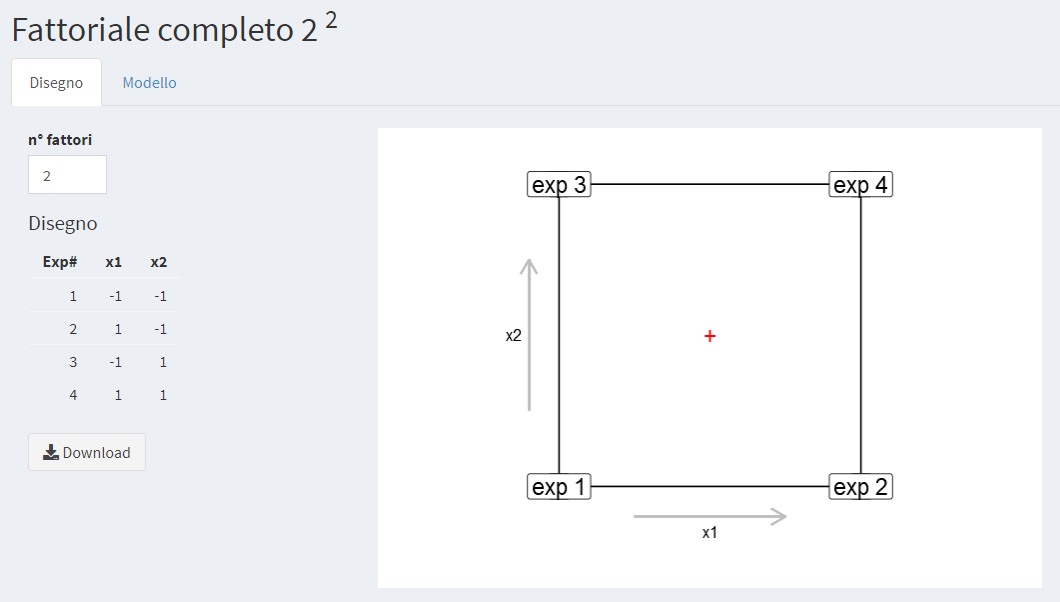
\includegraphics[width=1\linewidth]{Immagini/Fatt_compl/01_fattacompl2liv} 

}

\caption{Disegno fattoriale completo $2^2$}\label{fig:fc1}
\end{figure}

\begin{figure}

{\centering 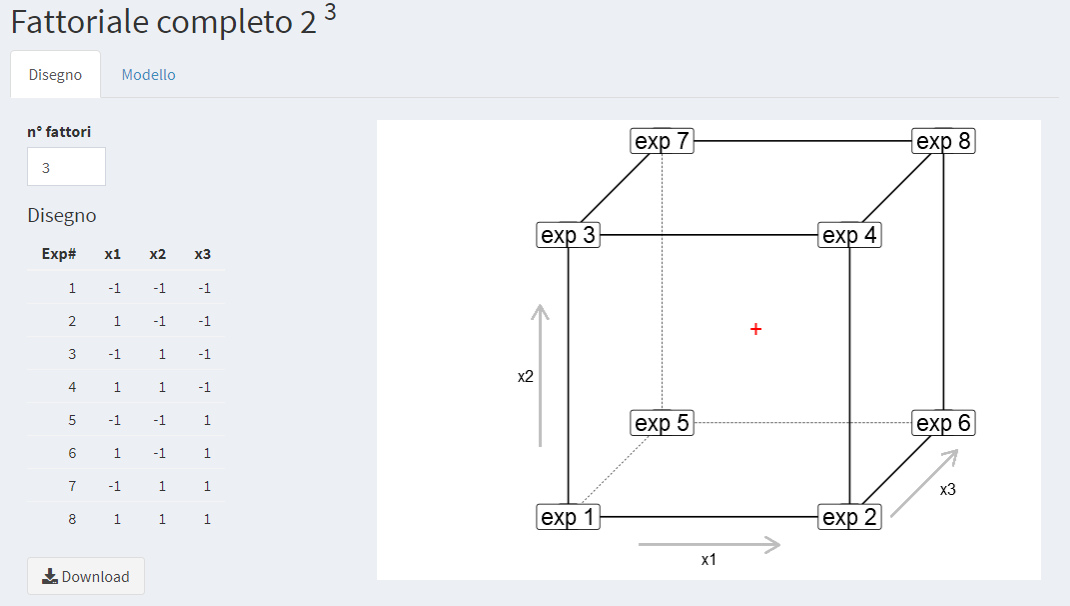
\includegraphics[width=1\linewidth]{Immagini/Fatt_compl/02_fattacompl3liv} 

}

\caption{Disegno fattoriale completo $2^3$}\label{fig:fc2}
\end{figure}

Consideriamo il modello lineare che tiene conto di tutti i termini
lineari e di tutte le possibili interazioni

\begin{equation}
y_i=\beta_0+\beta_1x_{i1}+\cdots+\beta_kx_{ik}+\beta_{12}x_{i1}x_{i2}+\cdots+\beta_{1\dots
k}x_{i1} \cdots x_{ik}+\epsilon_i, \qquad i=1,\dots,2^k, 
\label{eq:ModDisFull}
\end{equation}

dove \(\epsilon_i\sim N(0,\sigma^2)\) a due a due non correlate, errore
sperimentale.\newline La matrice \(X\) del modello è data dalla matrice in Tabella \ref{tab:MatrModDisFull}

\begin{longtable}[]{@{}crrrrrrrc@{}}
\caption{\label{tab:MatrModDisFull} Matrice modello \eqref{eq:ModDisFull}}\tabularnewline
\toprule
& \emph{Int.} & \(\bf{X_1}\) & \(\bf{X_2}\) & \(\cdots\) & \(\bf{X_k}\) & \(\bf{X_1X_2}\) & \(\cdots\) & \(\bf{X_1X_2\dots X_k}\)\tabularnewline
\midrule
\endfirsthead
\toprule
& \emph{Int.} & \(\bf{X_1}\) & \(\bf{X_2}\) & \(\cdots\) & \(\bf{X_k}\) & \(\bf{X_1X_2}\) & \(\cdots\) & \(\bf{X_1X_2\dots X_k}\)\tabularnewline
\midrule
\endhead
1 & 1 & -1 & -1 & \(\cdots\) & -1 & 1 & \(\cdots\) & \((-1)^k\)\tabularnewline
2 & 1 & 1 & -1 & \(\cdots\) & -1 & -1 & \(\cdots\) & \(\quad (-1)^{k-1}\)\tabularnewline
3 & 1 & -1 & 1 & \(\cdots\) & -1 & -1 & \(\cdots\) & .\tabularnewline
4 & 1 & 1 & 1 & \(\cdots\) & -1 & 1 & \(\cdots\) & .\tabularnewline
. & 1 & . & . & \(\cdots\) & . & . & \(\cdots\) & .\tabularnewline
. & 1 & . & . & \(\cdots\) & . & . & \(\cdots\) & .\tabularnewline
. & 1 & . & . & \(\cdots\) & . & . & \(\cdots\) & .\tabularnewline
. & 1 & -1 & -1 & \(\cdots\) & 1 & 1 & \(\cdots\) & .\tabularnewline
. & 1 & 1 & -1 & \(\cdots\) & 1 & -1 & \(\cdots\) & .\tabularnewline
. & 1 & -1 & 1 & \(\cdots\) & 1 & -1 & \(\cdots\) & .\tabularnewline
\(2^k\) & 1 & 1 & 1 & \(\cdots\) & 1 & 1 & \(\cdots\) & 1\tabularnewline
\bottomrule
\end{longtable}

Poiché la matrice del modello \eqref{eq:ModDisFull} è ortogonale, i
coefficienti relativi ad ogni termine lineare forniscono esattamente
l'informazione di quanto varia la risposta per uno spostamento unitario
del fattore relativo, ossia \(\frac{X_{max}-X_{min}}{2}\), mantenendo gli
altri parametri nulli. E' quindi 1/2 l'\textbf{effetto del parametro},
cioè la differenza tra la media dei valori delle risposte per \(X_{max}\)
e la media dei valori delle risposte per \(X_{min}\).\\
Nell'esempio numerico che trattiamo più avanti, l'effetto del parametro
\(X_1\) (temperatura), vedi Figura \ref{fig:fc5}, è dato dalla differenza
(23) tra la media (75.75) dei 4 valori della faccia \(X_1=1\) e la media
(52.75) dei 4 valori della faccia \(X_1=-1\). Il coefficiente di \(X_1\),
vedi Figura \ref{fig:fc6}, è esattamente 1/2 l'effetto della temperatura.

Più grande in valore assoluto è il coefficiente, e maggiore è l'effetto
del relativo fattore nel dominio sperimentale scelto.

Determinato il vettore \(y\) delle risposte, eseguendo i \(2^k\) esperimenti
nei punti sperimentali individuati dalla matrice sperimentale in
Tabella \ref{tab:MatrDisFull}. (\textbf{Nota importante:} per evitare effetto
di autocorrelazione nell'errore nel modello gli esperimenti non vanno
eseguiti nell'ordine in Tabella \ref{tab:MatrDisFull} ma vanno mischiati
casualmente) dobbiamo stimare

\begin{itemize}
\tightlist
\item
  \(1\) coefficiente interazione \(\beta_0\) (media delle \(2^k\) risposte)
\item
  \(k\) coefficienti termini lineari \(\beta_1,\cdots,\beta_k\)
\item
  in generale \(\frac{k!}{(k-m)!m!}\) coefficienti interazioni di ordine \(m\)
\end{itemize}

Si noti che per il binomio di Newton si ha che
\[
\sum_{m=0}^k\frac{k!}{(k-m)!m!}=2^k. 
\]
La matrice del modello, Tabella \ref{tab:MatrModDisFull}, è quindi un matrice
quadrata \(2^k\)x \(2^k\) e poiché le sue colonne sono a due a due
ortogonali è una matrice di Hadamard.

Dalla teoria della regressione sappiamo che uno stimatore del vettore
dei parametri \(\beta\) del modello \eqref{eq:ModDisFull} è dato dall'unica
soluzione del sistema \(y=Xb\) (si vedano le diapositive \emph{Fattoriale
completo})
\[
 b=X^{-1}y.
\]
e che
\[
Cov(b)=(X^tX)^{-1}=\frac{1}{2^k}I_k
\]
dove con \(I_k\) è indicata la matrice diagonale con valori tutti
uguali a \(1\) sulla diagonale (matrice identità).

Nell'applicativo, scelto il numero di fattori compaiono automaticamente
il modello e la matrice di dispersione (matrice \((X^tX)^{-1}\))
Figura \ref{fig:fc3}

\begin{figure}

{\centering 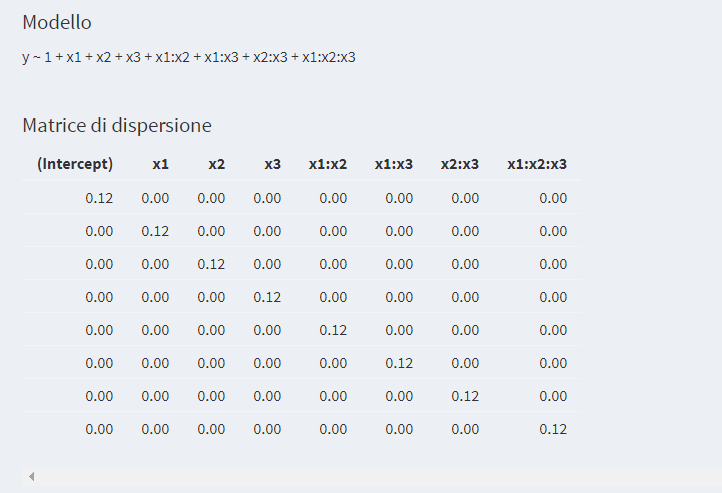
\includegraphics[width=1\linewidth]{Immagini/Fatt_compl/03_matr_disp} 

}

\caption{Modello e matrice di dispersione per un disegno fattoriale completo $2^3$}\label{fig:fc3}
\end{figure}

Come già osservato, la matrice di dispersione è una matrice diagonale, e
questo implica che tutti i fattori sono ortogonali tra di loro
\[
Corr(b_i,b_j)=0, \qquad i\neq j
\]
Il coefficiente \(\beta_j\) non cambia anche se elimino qualche
fattore, o anche tutti i fattori \(X_i,\) \(i\neq j\) dal modello (la
variazione dovuta da \(X_j\) sulla risposta è letta soltanto da
\(\beta_j\)).

Inoltre per lo stimatore \(b=X^{-1}y\) abbiamo che

\begin{equation}
Var(b_j)=\frac{\sigma^2}{2^k},
\qquad j=1,\dots,2^k 
\label{eq:VarFull}
\end{equation}

La \eqref{eq:VarFull} ci dice la qualità dell'informazione dello
stimatore \(b_j\). Ci permette inoltre di studiare la significatività
statistica di \(\beta_j\) nota la varianza sperimentale \(\sigma^2\).

Essendo \(y=Xb\) un sistema di \(2^k\) equazioni (linearmente indipendenti)
in \(2^k\) incognite, non abbiamo gradi di libertà, e quindi non siamo in
grado di stimare \(\sigma^2\). Alla fine di questo paragrafo vedremo, se
non è nota a priori la varianza \(\sigma^2\), come possiamo superare
questo ostacolo.

Il valore previsto dal modello in un punto \((x_1,x_2,\dots,x_k)\) del
dominio sperimentale è dato da
\[
\hat{y_0}=x_0b
\]
dove \(x_0=(1,x_1,\dots,x_1x_2,\dots,x_1x_2\cdots x_k)\) (riga della
matrice del modello Tabella \ref{tab:MatrDisFull} corrispondente al punto
\((x_1,x_2,\dots,x_k)\)). Dalla teoria sappiamo che la varianza dello
stimatore \(\hat{y_0}\) è data da
\[
Var(\hat{y_0})=x_0(X^tX)^{-1}x_0^t\sigma^2
\]
La quantità \(x_0(X^tX)^{-1}x_0^t\) è chiamata \emph{Leverage} nel punto
\((x_1,x_2,\dots,x_k)\).

Nell'applicativo si trova il grafico del leverage per ogni punto del
dominio, Figura \ref{fig:fc4}

\begin{figure}

{\centering 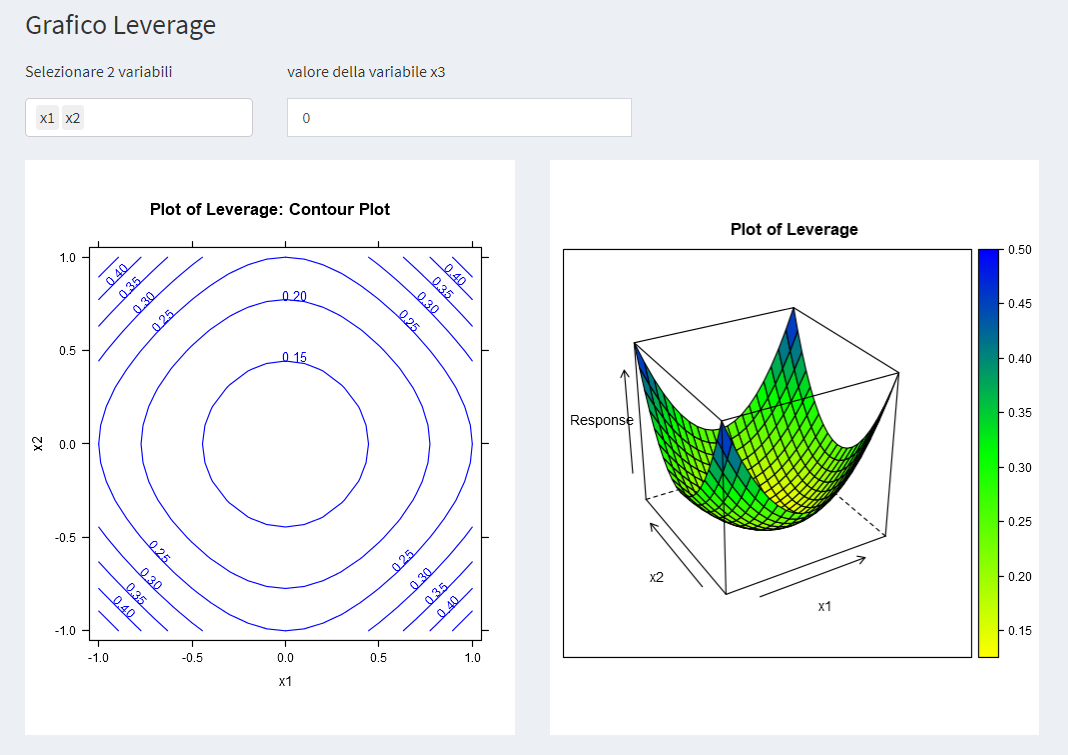
\includegraphics[width=1\linewidth]{Immagini/Fatt_compl/04_lev} 

}

\caption{Linee di livello e superficie del leverage per un disegno fattoriale completo $2^3$}\label{fig:fc4}
\end{figure}

La superficie di leverege ci dice com'è la qualità dell'informazione
dello stimatore risposta in ogni punto del dominio sperimentale.

A questo punto è opportuno fare due osservazioni importanti:

\begin{enumerate}
\def\labelenumi{\arabic{enumi})}
\item
  il leverage non dipende dai valori delle risposte. Per questo si
  trova nel sotto-menù \emph{Disegno} il cui output dipende solo dal
  disegno.
\item
  nei punti del disegno, poiché la somma dei quadrati dei valori delle
  righe della matrice del modello Tabella \ref{tab:MatrDisFull}è \(2^k\), il
  valore del leverage è \(1\).\\
  Questo significa che il modello ``deve passare'' per quei punti, ma
  questo non deve meravigliare poiché, coma già detto, non abbiamo
  gradi di libertà. Per fissare le idee su questo passaggio
  fondamentale, siamo nello stessa situazione che conosciamo nel piano
  quando abbiamo solo due punti per stimare i coefficienti di una
  retta.
\end{enumerate}

Si noti che i \(2^k\) punti sperimentali sono i punti del dominio
sperimentale di leverage massimo. Il che significa che in ognuno di
questi punti l'informazione che abbiamo grazie al modello è migliore di
quella che avremmo mediante un (unico) eventuale esperimento in quel
punto. Ciò significa che la risposta, o meglio l'aspettativa della
risposta, può essere predetta meglio (leggi con varianza minore) dal
modello che da un singolo esperimento in quel punto. \newline

Consideriamo ora un esempio numerico.\\
Supponiamo ora di dover identificare le condizioni di processo di una
reazione chimica. Vogliamo determinare l'influenza di 3 fattori

\begin{itemize}
\item
  \(X_1\): temperatura (°C)
\item
  \(X_2\): concentrazione del substrato (\%, p/p)
\item
  \(X_3\): tipo di catalizzatore
\end{itemize}

e delle loro interazioni sulla risposta

\begin{itemize}
\tightlist
\item
  \(Y\): resa di reazione
\end{itemize}

Dobbiamo innanzitutto scegliere il dominio sperimentale, cioè per ogni
fattore dobbiamo determinare un intervallo di valori compreso tra un
massimo e un minimo entro i quali studiare il fenomeno a cui siamo
interessati. Abbiamo 2 fattori quantitativi, che sono la temperatura e
la concentrazione del substrato, e un fattore qualitativo a 2 livelli, e
questo è il tipo di catalizzatore: A o B.

\begin{longtable}[]{@{}lrr@{}}
\caption{\label{tab:livelli}Definizione dei livelli}\tabularnewline
\toprule
Fattori & -1 & +1\tabularnewline
\midrule
\endfirsthead
\toprule
Fattori & -1 & +1\tabularnewline
\midrule
\endhead
temperatura & 160 & 180\tabularnewline
concentrazione & 20 & 40\tabularnewline
catalizzatore & A & B\tabularnewline
\bottomrule
\end{longtable}

La matrice del disegno Tabella \ref{tab:MatrDisFull} per 3 fattori è quella in Figura \ref{fig:fc2}. Il piano degli esperimenti Tabella \ref{tab:esperimenti} si
ottiene sostituendo a -1/+1 il valore corrispondente nella Tabella
\ref{tab:livelli}. \newpage

\begin{longtable}[]{@{}cccc@{}}
\caption{\label{tab:esperimenti}Piano degli esperimenti}\tabularnewline
\toprule
Exp. & Temp & Conc & Cat\tabularnewline
\midrule
\endfirsthead
\toprule
Exp. & Temp & Conc & Cat\tabularnewline
\midrule
\endhead
1 & 160 & 20 & A\tabularnewline
2 & 180 & 20 & A\tabularnewline
3 & 160 & 40 & A\tabularnewline
4 & 180 & 40 & A\tabularnewline
5 & 160 & 20 & B\tabularnewline
6 & 180 & 20 & B\tabularnewline
7 & 160 & 40 & B\tabularnewline
8 & 180 & 40 & B\tabularnewline
\bottomrule
\end{longtable}

Gli esperimenti sono elencati nel cosiddetto ``ordine standard''. Per
evitare di osservare effetti (errori) sistematici, gli esperimenti
devono essere eseguiti in ordine casuale (random order). Alla fine degli
esperimenti otteniamo i risultati in Tabella \ref{tab:esperimentir}

\begin{longtable}[]{@{}ccccc@{}}
\caption{\label{tab:esperimentir}Piano degli esperimenti con risposte}\tabularnewline
\toprule
Exp. & Temp & Conc & Cat & Resa\tabularnewline
\midrule
\endfirsthead
\toprule
Exp. & Temp & Conc & Cat & Resa\tabularnewline
\midrule
\endhead
1 & 160 & 20 & A & 60\tabularnewline
2 & 180 & 20 & A & 72\tabularnewline
3 & 160 & 40 & A & 54\tabularnewline
4 & 180 & 40 & A & 68\tabularnewline
5 & 160 & 20 & B & 52\tabularnewline
6 & 180 & 20 & B & 83\tabularnewline
7 & 160 & 40 & B & 45\tabularnewline
8 & 180 & 40 & B & 80\tabularnewline
\bottomrule
\end{longtable}

Per inserire le risposte nell'applicativo bisogna andare nel sotto menu
\emph{Modello} e inserire le risposte nell'apposito riquadro, vedi Figura
\ref{fig:fc5} (da Excel basta copiare la colonna delle risposte e
incollarla nel riquadro)

\begin{figure}

{\centering 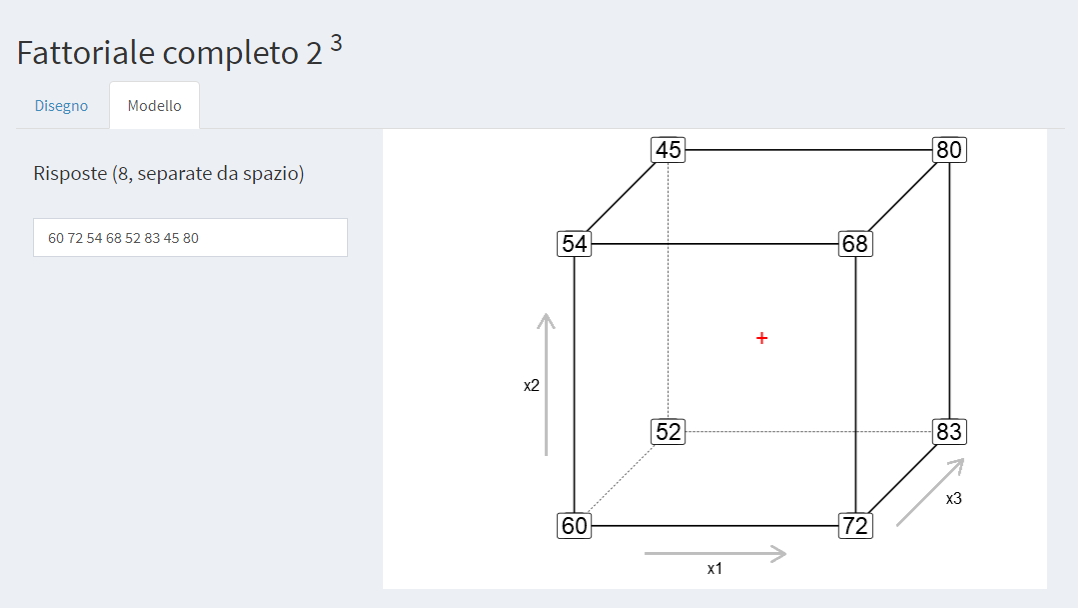
\includegraphics[width=1\linewidth]{Immagini/Fatt_compl/05_risp} 

}

\caption{Inserimento risposte nell'applicativo}\label{fig:fc5}
\end{figure}

Per un numero di fattori non superiore a 3 viene fornita anche una
rappresentazione grafica delle risposte.

Una volta inserite le risposte, il calcolo dei coefficienti del modello
è automatico e ne abbiamo anche una rappresentazione grafica, vedi
Figura \ref{fig:fc6}

\begin{figure}

{\centering 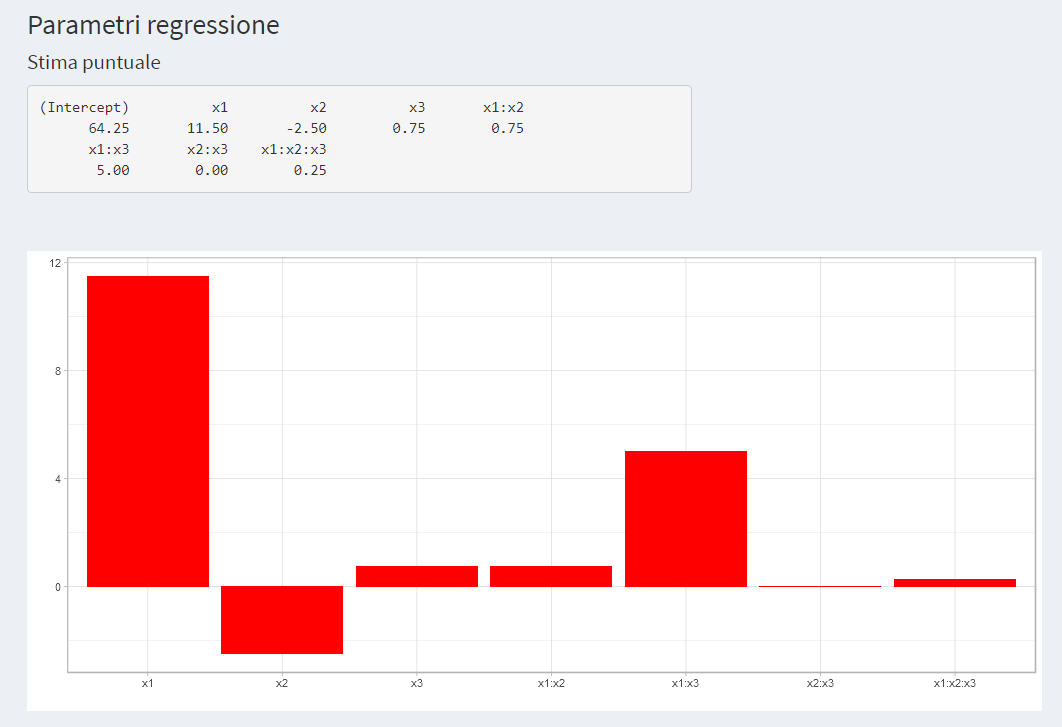
\includegraphics[width=1\linewidth]{Immagini/Fatt_compl/06_coeff} 

}

\caption{Calcolo dei coefficienti del modello}\label{fig:fc6}
\end{figure}

Un altro grafico riportato è il \emph{Grafico degli effetti normalizzati},
Figura \ref{fig:fc7}, in cui sono rappresentati i coefficienti che
contribuiscono di più nel determinare la risposta. Il grafico
rappresenta la percentuale del contributo di ciascun coefficiente
elevato al quadrato alla somma dei quadrati di tutti i coefficienti. I
coefficienti che risultano dare un contributo in percentuale maggiore
sono quelli che che influenzano maggiormente la risposta.

\begin{figure}

{\centering 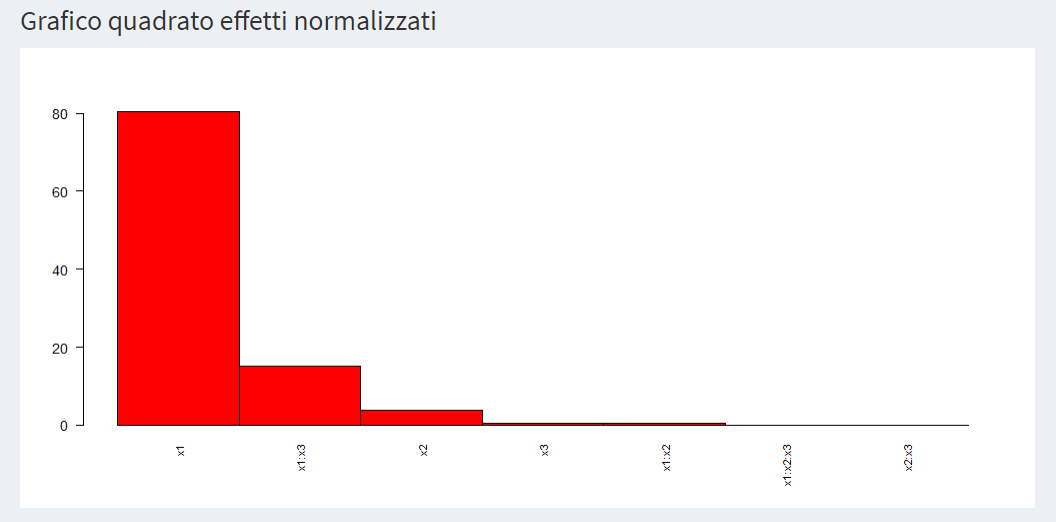
\includegraphics[width=1\linewidth]{Immagini/Fatt_compl/07_coeff_norm} 

}

\caption{Grafico degli effetti normalizzati}\label{fig:fc7}
\end{figure}

Dai grafici Figura \ref{fig:fc6} e Figura \ref{fig:fc7} risulta che i fattori
che influenzano di più la risposta Resa sono la temperatura e la sua
interazione con il tipo di catalizzatore.\\
In Figura \ref{fig:fc8} è illustrato il grafico della superficie di
risposta della Resa in funzione della temperatura e del tipo di
catalizzatore, avendo fissato la concentrazione del substrato nel punto
centrale del suo intervallo di variazione, vale a dire al 30\%.

\begin{figure}

{\centering 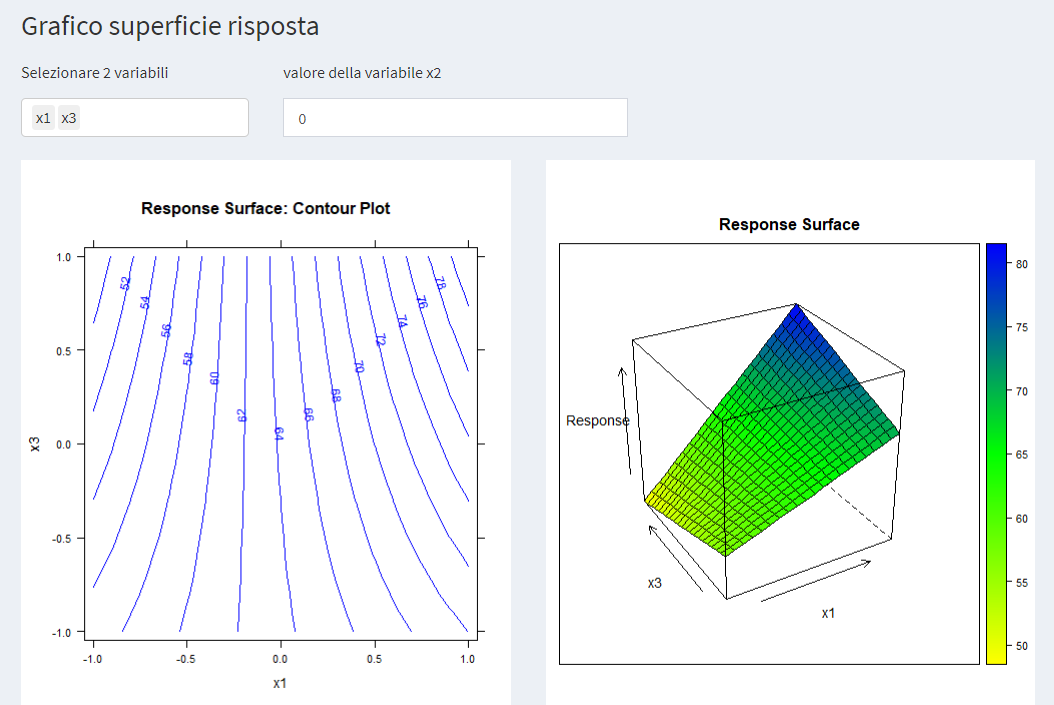
\includegraphics[width=1\linewidth]{Immagini/Fatt_compl/08_sup_risp} 

}

\caption{Grafico della superficie di risposta della Resa}\label{fig:fc8}
\end{figure}

Come si nota dalla Figura \ref{fig:fc8} il massimo della resa si ottiene
alla temperatura massima (180 °C) e usando il catalizzatore del tipo B
quando il substrato è alla concentrazione del 30\%.

Circa la significatività dei coefficienti, per quanto già osservato
precedentemente, non abbiamo gradi di libertà e quindi non è possibile
stimare \(\sigma^2\).

Una analisi grafica della significatività dei parametri \(b_j\) può essere
effettuata mediante il \emph{Normal Probability Plot}, Figura \ref{fig:fc9}. Se
tutti i coefficienti fossero nulli, i.e.~se fossero tutti distribuiti
come una normale di media \(0\) e varianza \(\sigma^2/2^k\), essi sarebbero
distribuiti come una retta. Possiamo considerare significativamente non
nulli i coefficienti che si discostano dalla retta.

\begin{figure}

{\centering 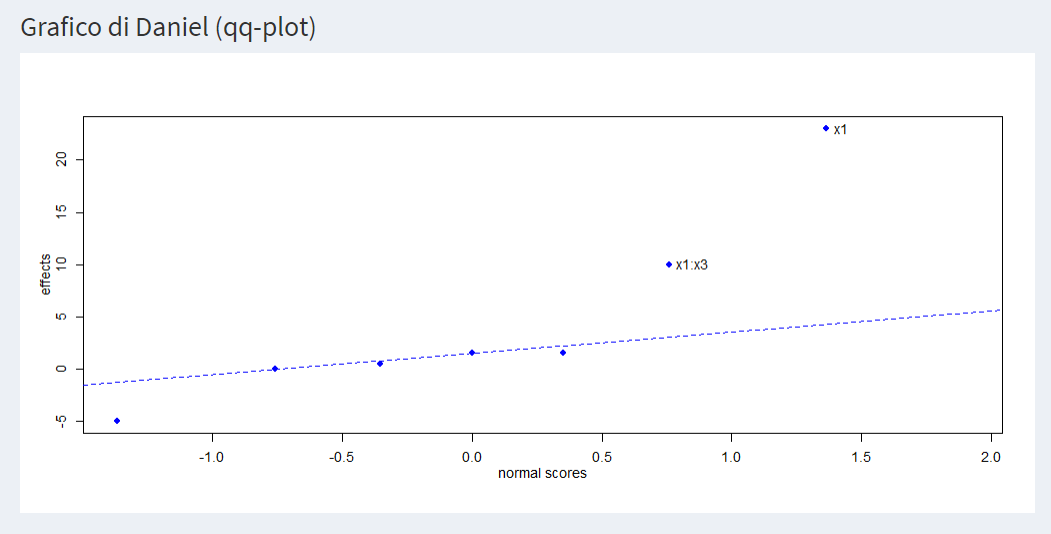
\includegraphics[width=1\linewidth]{Immagini/Fatt_compl/09_qqplot} 

}

\caption{qq-plot dei coefficienti}\label{fig:fc9}
\end{figure}

Dal qq-plot in Figura \ref{fig:fc9} si ottiene la conferma che sono
significativi (leggi: diversi da zero) la temperatura e la sua
interazione con il tipo di catalizzatore.

Per convalidare il modello eseguiamo alcune misure indipendenti
\(\eta_1,\dots,\eta_p\) in un punto del dominio scelto arbitrariamente. In
generale si prende il centro del dominio perché è il punto in cui il
leverage è minore. Possiamo determinare \(\sigma^2\) con lo stimatore \[
s^2=\frac{1}{p-1}\sum_{p=1}^p(\eta_i-\bar{\eta})^2.
\] Possiamo costruire l'intervallo di confidenza della misura ``vera'' in
quel punto \[
\bar{\eta}\pm t(\alpha/2,p-1)s\sqrt{1/p}
\] per \(\alpha\) fissato (in generale \(\alpha=95\%\)).

Nel nostro caso essendo il terzo fattore qualitativo prendiamo il punto
centrale tra la temperatura e la concentrazione per il catalizzatore di
tipo B, ossia il punto \((X_1,X_2,X_3)=(0,0,1)\).\\
Inserendo il valore delle misure indipendenti nell'applicativo,
Figura \ref{fig:fc10} otteniamo il valore medio delle misure e il relativo
intervallo di confidenza al 95\%, quindi il valore della deviazione
standard e dei gradi di libertà.

\begin{figure}

{\centering 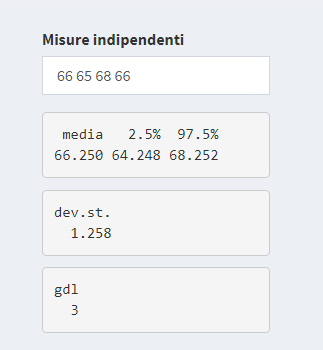
\includegraphics[width=1\linewidth]{Immagini/Fatt_compl/10_mis_ind} 

}

\caption{Misure indipendenti}\label{fig:fc10}
\end{figure}

Inserendo le misure indipendenti abbiamo quindi una stima di \(\sigma\) e
dei gradi di libertà. Utilizzando questi valori è possibile, grazie
all'equazione \eqref{eq:VarFull}, costruire l'intervallo di confidenza dei
parametri del modello. Nell'applicativo si ottengono gli estremi degli
intervalli di confidenza dei parametri per alcuni valori di \(\alpha\) e i
relativi \(p-value\), Figura \ref{fig:fc11}

\begin{figure}

{\centering 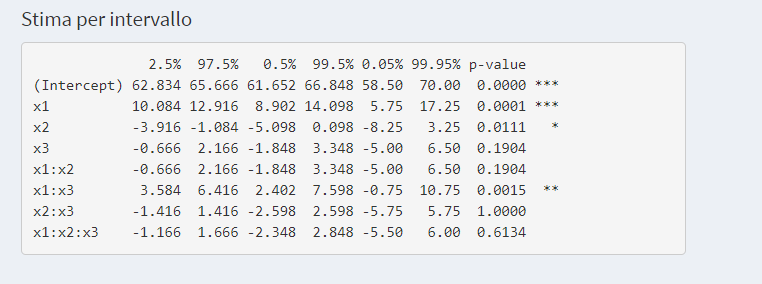
\includegraphics[width=1\linewidth]{Immagini/Fatt_compl/11_intconf} 

}

\caption{Estremi degli intervalli di confidenza dei coefficienti}\label{fig:fc11}
\end{figure}

Nel grafico dei parametri, l'ampiezza degli intervalli di confidenza è
rapprentata con un segmento di colore verde, Figura \ref{fig:fc12}

\begin{figure}

{\centering 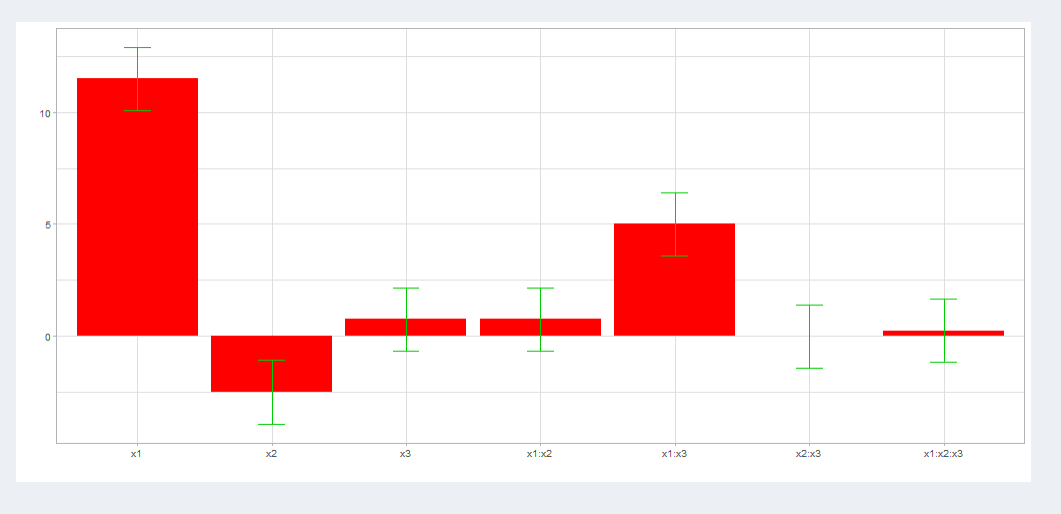
\includegraphics[width=1\linewidth]{Immagini/Fatt_compl/12_intcong_graf} 

}

\caption{Grafico dei coefficienti con estrremi degli intervalli di confidenza dei coefficienti}\label{fig:fc12}
\end{figure}

Per convalidare il modello bisogna quindi vedere quale è il valore
previsto dal modello nel punto in cui abbiamo eseguito le misure
indipendenti e verificare che non differisca significativamente dal
valore ottenuto dalle misure indipendenti (ossia appartenga
all'intervallo di confidenza determinato).\\
Inserendo nell'applicativo le coordinate del punto in cui sono state
eseguite le misure indipendenti otteniamo la previsione del modello in
quel punto e gli estremi dell'intervallo di confidenza costruiti con la
stima di \(\sigma\) ottenuta, Figura \ref{fig:fc13}

\begin{figure}

{\centering 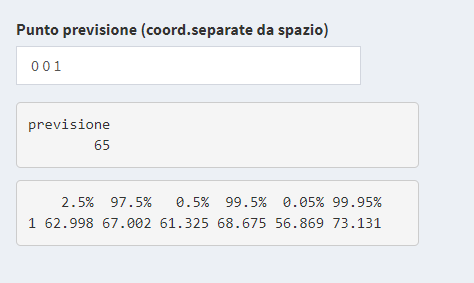
\includegraphics[width=1\linewidth]{Immagini/Fatt_compl/13_prev} 

}

\caption{Previsione del modello in un punto}\label{fig:fc13}
\end{figure}

Nel nostro esempio numerico il modello risulta convalidato.

\hypertarget{disegni-frazionari}{%
\chapter{Disegni Frazionari}\label{disegni-frazionari}}

All'aumentare del numero \(k\) dei fattori, il numero degli esperimenti da eseguire in un disegno fattoriale completo (a 2 livelli) aumenta esponenzialmente come \(2^k\).\\
In Tabella \ref{tab:exprich} è riportato il numero di esperimenti richiesti in funzione del numero di fattori \(k\) nei piani sperimentali fattoriali completi.

\begin{table}

\caption{\label{tab:exprich}Esperimenti richiesti per disegni fattoriali completi $2^k$}
\centering
\begin{tabular}[t]{cc}
\toprule
Fattori (k) & Esperimenti (2\textasciicircum{}k)\\
\midrule
4 & 16\\
5 & 32\\
6 & 64\\
7 & 128\\
8 & 256\\
\addlinespace
9 & 512\\
\bottomrule
\end{tabular}
\end{table}

E' possibile ridurre il numero di esperimenti, riducendolo di \(\frac{1}{2},\frac{1}{4}, \dots\), costruendo a partire da un disegno fattoriale completo \(2^k\) un disegno fattoriale frazionario \(2^{k-p}\) pur di accettare di ``confondere'' tra loro alcuni termini del modello. In generale, la strategia per fare questo consiste nel cercare di ``confondere'' termini di ordine maggiore che possono essere considerati trascurabili a priori, secondo il principio empirico della economia degli effetti (v. \protect\hyperlink{glossario}{Glossario}).

Vediamo come possiamo costruire un disegno frazionario \(2^{k-p}\) con un esempio specifico.\\
Supponiamo di voler costruire il disegno \(2^{5-2}\) ossia \(1/4\) del disegno fattoriale completo \(2^5\).\\
Partiamo dal disegno \(2^3\), vedi Tabella \ref{tab:fatt3}

\begin{table}

\caption{\label{tab:fatt3}Disegno fattorialo completo $2^3$}
\centering
\begin{tabular}[t]{rrr}
\toprule
x1 & x2 & x3\\
\midrule
-1 & -1 & -1\\
1 & -1 & -1\\
-1 & 1 & -1\\
1 & 1 & -1\\
-1 & -1 & 1\\
\addlinespace
1 & -1 & 1\\
-1 & 1 & 1\\
1 & 1 & 1\\
\bottomrule
\end{tabular}
\end{table}

a cui dobbiamo aggiungere i fattori mancanti \(x_4\) e \(x_5\) ``confondendoli'' con le interazioni \(x_4=x_1x_2\) e \(x_5=x_1x_3\). Otteniamo così il disegno Tabella \ref{tab:fraz52} in cui la quarta colonna risulta il prodotto della prima con seconda e la quinta il prodotto tra la prima e la terza \newpage

\begin{table}

\caption{\label{tab:fraz52}Disegno frazionario $2^{5-2}$}
\centering
\begin{tabular}[t]{rrrrr}
\toprule
x1 & x2 & x3 & x4 & x5\\
\midrule
-1 & -1 & -1 & 1 & 1\\
1 & -1 & -1 & -1 & -1\\
-1 & 1 & -1 & -1 & 1\\
1 & 1 & -1 & 1 & -1\\
-1 & -1 & 1 & 1 & -1\\
\addlinespace
1 & -1 & 1 & -1 & 1\\
-1 & 1 & 1 & -1 & -1\\
1 & 1 & 1 & 1 & 1\\
\bottomrule
\end{tabular}
\end{table}

Diremo che \(x_4=x_1x_2\) e \(x_5=x_1x_3\) sono i generatori del disegno frazionario \(2^{5-2}\).

Nell'applicativo, nel menù \emph{Frazionario}, vengono costruiti i disegni frazionari \(2^{k-p}\) indicando il numero di fattori \(k\) e il numero di generatori \(p\).\\
In Figura \ref{fig:fz1} abbiamo il risultato che si ottiene per \(k=5\) e \(p=2\), ossia il disegno \(2^{5-2}\).

\begin{figure}[ht]

{\centering 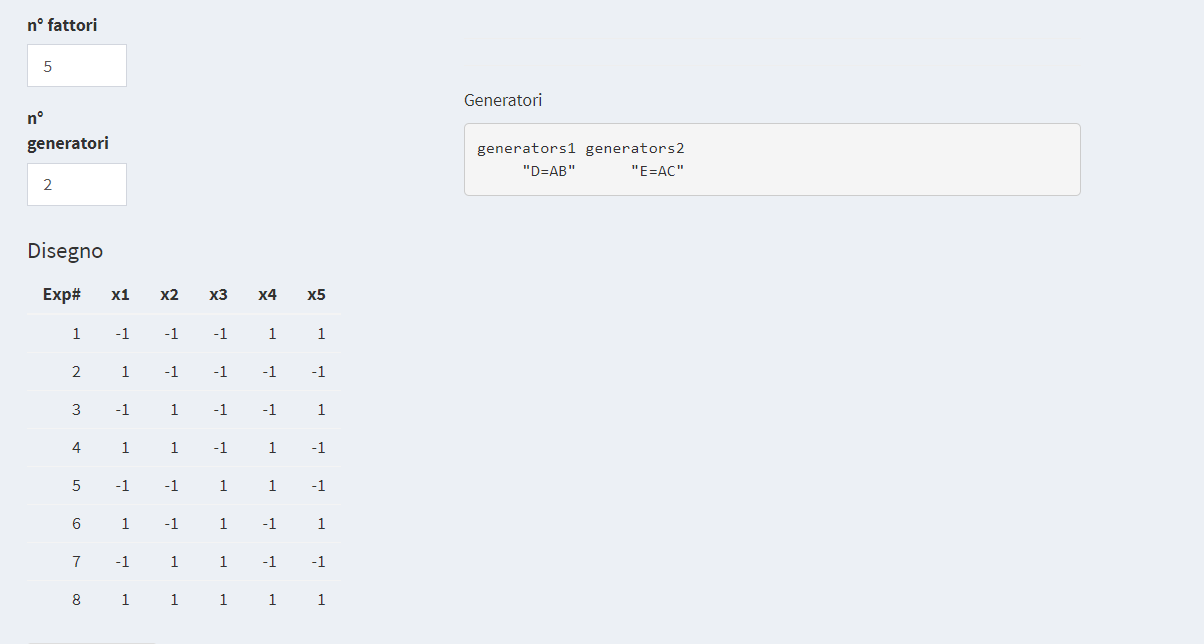
\includegraphics[width=1\linewidth]{Immagini/Fraz/01_fraz} 

}

\caption{Disegno frazionario $2^{5-2}$}\label{fig:fz1}
\end{figure}

Si noti che i generatori sono indicati con le lettere maiuscole, e che queste corrispondono alle colonne della matrice disposte in ordine alfabetico (A è la prima colonna, B la seconda, C la terza, D la quarta ed E la quinta colonna)

Poiché ogni colonna della matrice del disegno elevata al quadrato è la colonna cosiddetta \emph{identità}, \emph{Int.}, costituita solo da valori uguali a 1, dalle relazioni \(x_4=x_1x_2\) e \(x_5=x_1x_3\) si ottiene facilmente che

\[
Int.=x_1x_2x_4 \qquad  \rm{e} \qquad \it{Int.} = x_1x_3x_5 
\]

dette \emph{Relazioni di identità}. La lunghezza (ordine delle interazioni) minima delle relazioni d'identità è chiamata \emph{risoluzione} del disegno e, di solito, è indicata con un numero romano. Nel nostro esempio la risoluzione è \(III\) e il disegno viene indicato con \(2^{5-2}_{III}\).\\
In linea di principio conviene scegliere relazioni di risoluzione massima (V e superiore) in quanto confondono termini di ordine maggiore. Questa di solito è l'indicazione data dalla maggior parte dei software professionali commerciali (v. Figura \ref{fig:fz2}). Ma affinando l'esperienza e la pratica nell'uso dei fattoriali frazionari si constateranno le notevoli potenzialità offerte anche da disegni di ordine III e IV.

Nella Figura \ref{fig:fz2}, è riportata la copia della prima schermata da Design Expert®: sono indicati i disegni frazionari che si possono costruire in funzione del numero di fattori (per colonna) e numero di esperimenti (per riga) con la relativa risoluzione.

\begin{figure}[ht]

{\centering 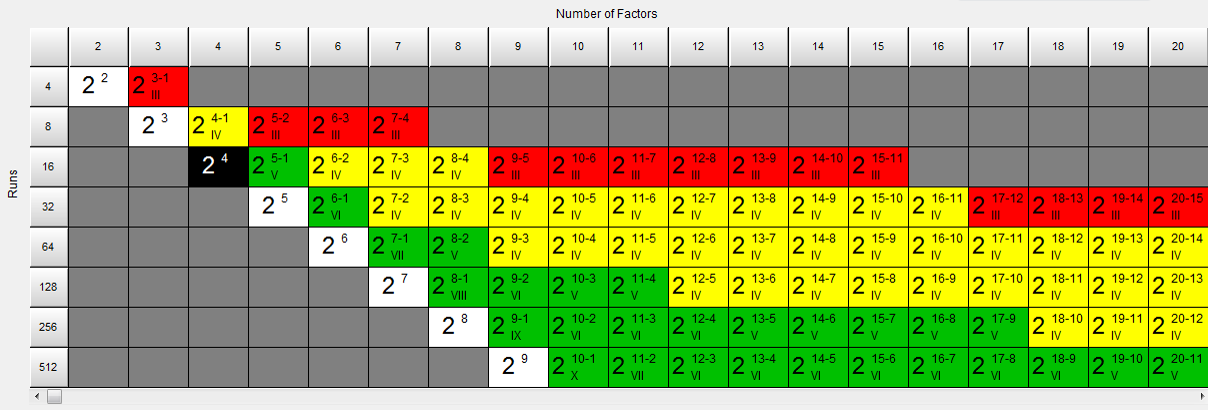
\includegraphics[width=1\linewidth]{Immagini/Fraz/02_risoluzione} 

}

\caption{Disegni frazionari con risoluzione}\label{fig:fz2}
\end{figure}

Per la ragione detta sopra, i programmatori di Design Expert® hanno assegnato dei codici-colore ``semaforici'' ai diversi disegni frazionari. Il colore del riquadro corrisponde al rischio di ottenere risultati inconcludenti. Perciò disegni con risoluzione \(III\), in cui si ``confondono'' i termini lineari con le interazioni di ordine 2 sono colorati in rosso (rischio/attenzione alti); i disegni di risoluzione \(IV\) in cui si ``confondono'' i termini lineari con le interazioni di ordine 3, e le interazioni di ordine 2 sono confuse a coppie tra loro, sono in giallo (rischio/attenzione medi). In verde, invece, sono indicati i disegni di risoluzione superiore a V (via libera, nessuna attenzione?). Questo tipo di classificazione è discutibile, come detto, ed è da considerare al pari di un consiglio di prudenza, peraltro scontato, perché l'uso dei fattoriali frazionari è da pensare per risolvere il problema chimico in esame, e non viceversa (i.e.~come adattare il problema ad un disegno frazionario di risoluzione sufficientemente alta).
La Figura \ref{fig:fz2} è la prima immagine del menù \emph{Frazionari} dell'applicativo.

Con semplice algebra, sempre osservando che \(x_i^2=Int.\), i.e.~ogni colonna al quadrato è la colonna identità \(Int.\) formata da tutti 1, si ottengono tutte le altre ``confusioni''.\\
Nell'applicativo compaiono automaticamente sia il modello relativo al disegno sia tutte le ``confusioni'', vedi Figura \ref{fig:fz3}

\begin{figure}[ht]

{\centering 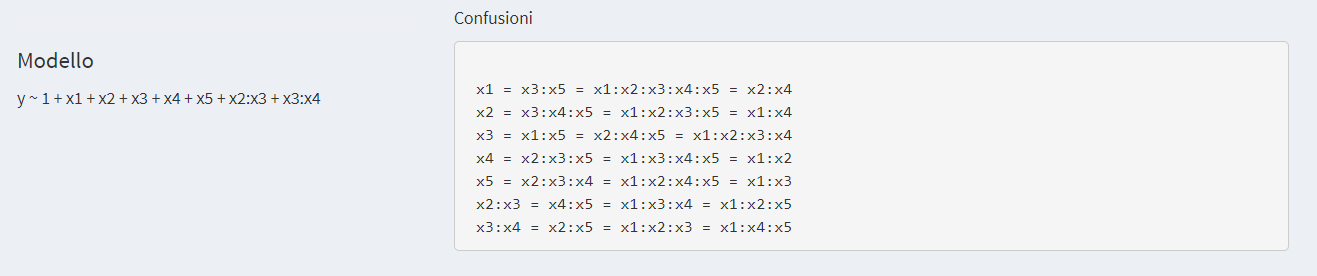
\includegraphics[width=1\linewidth]{Immagini/Fraz/03_confusioni} 

}

\caption{Modello e confusioni del disegno frazionario $2_{III}^{5-2}$}\label{fig:fz3}
\end{figure}

Per quanto riguarda la rimanente parte di output, tutto è presentato nella stessa logica già vista per i disegni fattoriali completi.

\hypertarget{esempio-confusioni}{%
\section{Esempio: confusioni}\label{esempio-confusioni}}

Per comprendere meglio le ``confusioni'' in un disegno frazionario consideriamo il seguente esempio didattico. Supponiamo che il modello ``vero'' (quello che a priori non conosciamo) del fenomeno di studio sia il seguente
\[
y=x_1+5x_2-3x_3+15x_1x_3+\epsilon
\]
Nella progettazione degli esperimenti per studiare il fenomeno in osservazione abbiamo ipotizzato che la risposta dipenda da 5 fattori \(x_1,x_2,x_3,x_4,x_5\).

Per studiare tutte le possibili interazioni consideriamo un disegno fattoriale completo Tabella \ref{tab:Conffull}

\begin{table}

\caption{\label{tab:Conffull}Disegno fattoriale completo $2^5$ (32 esperimenti) con risposte costruito dal modello "vero" ipotizzato $y=x_1+5x_2-3x_3+15x_1x_3+\epsilon$}
\centering
\begin{tabular}[t]{rrrrrr}
\toprule
x1 & x2 & x3 & x4 & x5 & y\\
\midrule
-1 & -1 & -1 & -1 & -1 & 11.96\\
1 & -1 & -1 & -1 & -1 & -17.15\\
-1 & 1 & -1 & -1 & -1 & 23.23\\
1 & 1 & -1 & -1 & -1 & -5.04\\
-1 & -1 & 1 & -1 & -1 & -22.91\\
\addlinespace
1 & -1 & 1 & -1 & -1 & 5.90\\
-1 & 1 & 1 & -1 & -1 & -12.81\\
1 & 1 & 1 & -1 & -1 & 18.18\\
-1 & -1 & -1 & 1 & -1 & 11.56\\
1 & -1 & -1 & 1 & -1 & -17.82\\
\addlinespace
-1 & 1 & -1 & 1 & -1 & 20.86\\
1 & 1 & -1 & 1 & -1 & -6.44\\
-1 & -1 & 1 & 1 & -1 & -24.14\\
1 & -1 & 1 & 1 & -1 & 9.41\\
-1 & 1 & 1 & 1 & -1 & -13.74\\
\addlinespace
1 & 1 & 1 & 1 & -1 & 16.17\\
-1 & -1 & -1 & -1 & 1 & 11.64\\
1 & -1 & -1 & -1 & 1 & -14.71\\
-1 & 1 & -1 & -1 & 1 & 20.62\\
1 & 1 & -1 & -1 & 1 & -5.95\\
\addlinespace
-1 & -1 & 1 & -1 & 1 & -23.92\\
1 & -1 & 1 & -1 & 1 & 7.07\\
-1 & 1 & 1 & -1 & 1 & -13.31\\
1 & 1 & 1 & -1 & 1 & 17.66\\
-1 & -1 & -1 & 1 & 1 & 11.69\\
\addlinespace
1 & -1 & -1 & 1 & 1 & -15.81\\
-1 & 1 & -1 & 1 & 1 & 21.73\\
1 & 1 & -1 & 1 & 1 & -4.59\\
-1 & -1 & 1 & 1 & 1 & -24.53\\
1 & -1 & 1 & 1 & 1 & 6.81\\
\addlinespace
-1 & 1 & 1 & 1 & 1 & -13.02\\
1 & 1 & 1 & 1 & 1 & 18.17\\
\bottomrule
\end{tabular}
\end{table}

Il cui grafico dei coefficienti è dato in Figura \ref{fig:fz11}.

\begin{figure}[ht]

{\centering 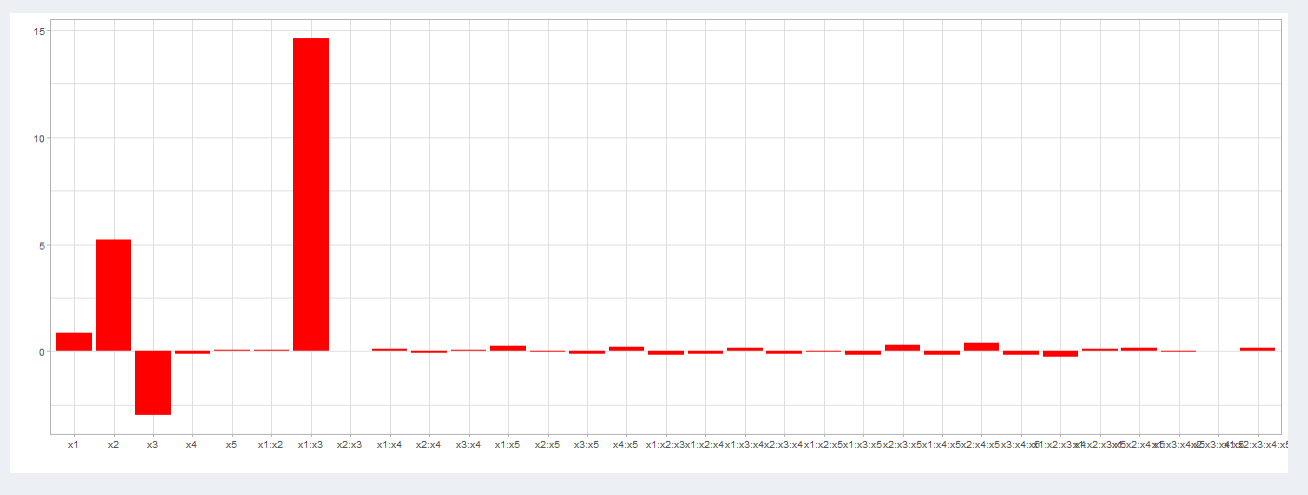
\includegraphics[width=1\linewidth]{Immagini/Fraz/11_Conf_full2} 

}

\caption{Grafico dei coefficienti del modello $2^5$ }\label{fig:fz11}
\end{figure}

Per ridurre della metà il numero di esperimenti si considera un disegno frazionario \(2^{5-1}_V\), Tabella \ref{tab:Confris5}
\newpage

\begin{table}

\caption{\label{tab:Confris5}Disegno frazionario $2^{5-1}_V$ (16 esperimenti) con risposte costruito dal modello supposto $y=x_1+5x_2-3x_3+15x_1x_3+\epsilon$}
\centering
\begin{tabular}[t]{rrrrrr}
\toprule
x1 & x2 & x3 & x4 & x5 & y\\
\midrule
-1 & -1 & -1 & -1 & 1 & 11.64\\
1 & -1 & -1 & -1 & -1 & -17.15\\
-1 & 1 & -1 & -1 & -1 & 23.23\\
1 & 1 & -1 & -1 & 1 & -5.95\\
-1 & -1 & 1 & -1 & -1 & -22.91\\
\addlinespace
1 & -1 & 1 & -1 & 1 & 7.07\\
-1 & 1 & 1 & -1 & 1 & -13.31\\
1 & 1 & 1 & -1 & -1 & 18.18\\
-1 & -1 & -1 & 1 & -1 & 11.56\\
1 & -1 & -1 & 1 & 1 & -15.81\\
\addlinespace
-1 & 1 & -1 & 1 & 1 & 21.73\\
1 & 1 & -1 & 1 & -1 & -6.44\\
-1 & -1 & 1 & 1 & 1 & -24.53\\
1 & -1 & 1 & 1 & -1 & 9.41\\
-1 & 1 & 1 & 1 & -1 & -13.74\\
\addlinespace
1 & 1 & 1 & 1 & 1 & 18.17\\
\bottomrule
\end{tabular}
\end{table}

In questo caso il grafico dei parametri è dato da Figura \ref{fig:fz12}

\begin{figure}[ht]

{\centering 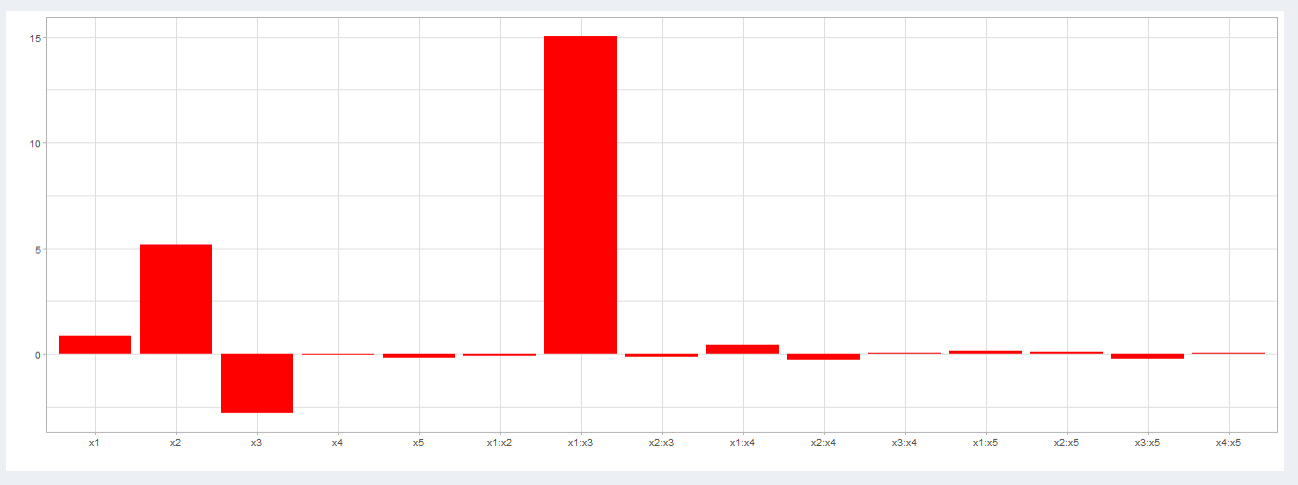
\includegraphics[width=1\linewidth]{Immagini/Fraz/12_Conf_ris5} 

}

\caption{Grafico dei coefficienti del modello frazionario $2^{5-1}_V$ }\label{fig:fz12}
\end{figure}

\newpage

Il disegno scelto ha risoluzione \(V\), ciò significa che i termini lineari sono confusi con le interazioni di ordine 4 e quindi posssiamo supporre che il valore di ciascun parametro si riferisca al termine lineare corrispondente (consideriamo trascurabili tutte le interazioni di ordine 4). E' possibile fare un ragionamento analogo per le interazioni di ordine 2 che si confondono con le interazioni di ordine 3. Supponendo che queste ultime siano trascurabili, possiamo dunque concludere che il valore di ciascun parametro di interazione si riferisca easclusivamente alle interazioni di ordine 2.

Se si volesse diminuire ulteriormente il numero di esperimenti, è possibile ricorrere ad un disegno frazionario \(2^{5-2}_{III}\), Tabella \ref{tab:Confris3}

\begin{table}

\caption{\label{tab:Confris3}Disegno frazionario $2^{5-2}_{III}$ (8 esperimenti) con risposte costruito dal modello supposto $y=x_1+5x_2-3x_3+15x_1x_3+\epsilon$}
\centering
\begin{tabular}[t]{rrrrrr}
\toprule
x1 & x2 & x3 & x4 & x5 & y\\
\midrule
-1 & -1 & -1 & 1 & 1 & 11.69\\
1 & -1 & -1 & -1 & -1 & -17.15\\
-1 & 1 & -1 & -1 & 1 & 20.62\\
1 & 1 & -1 & 1 & -1 & -6.44\\
-1 & -1 & 1 & 1 & -1 & -24.14\\
\addlinespace
1 & -1 & 1 & -1 & 1 & 7.07\\
-1 & 1 & 1 & -1 & -1 & -12.81\\
1 & 1 & 1 & 1 & 1 & 18.17\\
\bottomrule
\end{tabular}
\end{table}

Questo è un disegno di risoluzione \(III\), bisogna quindi fare molta attenzione alle confusioni Figura \ref{fig:fz13}

\begin{figure}[ht]

{\centering 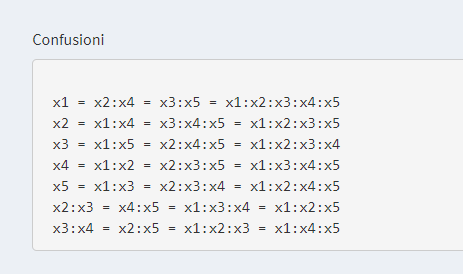
\includegraphics[width=1\linewidth]{Immagini/Fraz/13_Conf_ris3} 

}

\caption{Confusioni del disegno $2^{5-2}_{III}$}\label{fig:fz13}
\end{figure}

I termini lineari si confondono con le interazione di ordine 2. Come si vede dal grafico dei coefficienti Figura \ref{fig:fz14}

\begin{figure}[ht]

{\centering 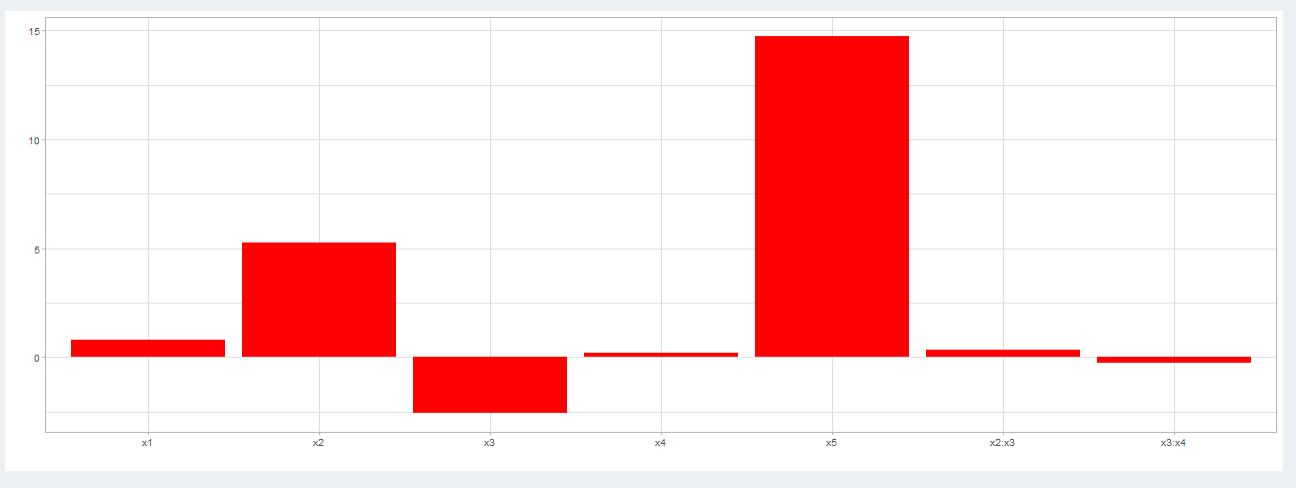
\includegraphics[width=1\linewidth]{Immagini/Fraz/14_Conf_ris3} 

}

\caption{Grafico dei coefficienti del disegno $2^{5-2}_{III}$}\label{fig:fz14}
\end{figure}

ad esempio il valore di \(x_5\) è circa 15, ma non siamo in grado di stabilire se è dovuto dal termine linerare \(x_5\), dal termine ``confuso'' \(x_1x_3\) (come in questo caso, ricordo la forma del modello \(y=x_1+5x_2-3x_3+15x_1x_3+\epsilon\)) o dalla combinazione di entrambi.

\hypertarget{esempio-studio-dei-fattori-dellestrazione-liquido-liquido}{%
\section{Esempio: studio dei fattori dell'estrazione liquido-liquido}\label{esempio-studio-dei-fattori-dellestrazione-liquido-liquido}}

Per meglio comprendere i disegni frazionari e l'utilizzo dell'applicativo in questi disegni consideriamo il seguente esempio.

Si vogliono studiare i seguenti 4 fattori:

\begin{itemize}
\item
  volume miscela solventi per estrazione
\item
  tempo di centrifuga dell'estratto
\item
  forza ionica del campione (quantità di NaCl da aggiungere)
\item
  tempo di estrazione
\end{itemize}

Definiamo innanzitutto il dominio sperimentale. Per ogni fattore determiniamo l'intervallo di valori compreso tra un massimo e un minimo entro i quali studiare il fenomeno, Tabella \ref{tab:fzliv}

\begin{table}

\caption{\label{tab:fzliv}Definizione dei livelli}
\centering
\begin{tabular}[t]{lcc}
\toprule
Fattori & -1 & +1\\
\midrule
vol. solvente & 10 & 40\\
t. centrifuga & 5 & 20\\
forza ionica & 1 & 5\\
t. estrazione & 1 & 5\\
\bottomrule
\end{tabular}
\end{table}

Il piano fattoriale completo prevede 16 esperimenti. L'impegno del laboratorio è considerato troppo oneroso. Si decide quindi di utilizzare un disegno frazionario \(2^{4-1}_{IV}\) per eseguire la metà degli esperimenti. Vedi Figura \ref{fig:fz4}

\begin{figure}[ht]

{\centering 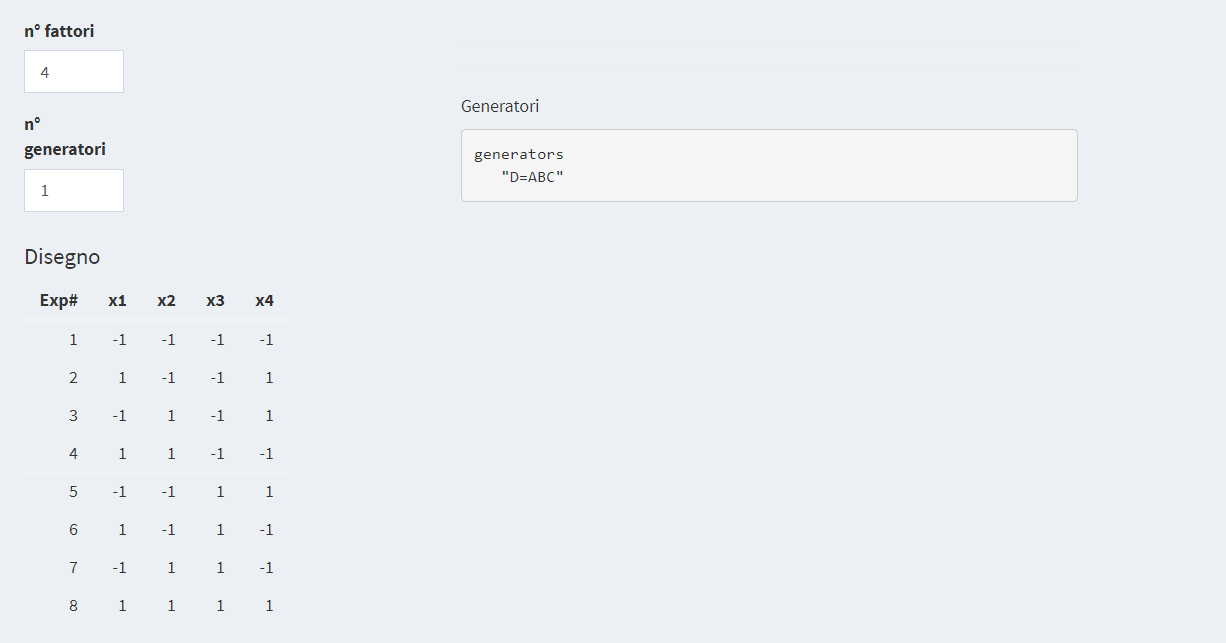
\includegraphics[width=1\linewidth]{Immagini/Fraz/04_esempio1} 

}

\caption{Disegno e generatore di  $2_{IV}^{4-1}$}\label{fig:fz4}
\end{figure}

Il piano sperimentale risulta quindi Tabella \ref{tab:piano}
\newpage

\begin{table}

\caption{\label{tab:piano}Piano sperimentale}
\centering
\begin{tabular}[t]{cccc}
\toprule
vol. solvente & t. centrifuga & forza ionica & t. estrazione\\
\midrule
10 & 5 & 1 & 1\\
40 & 5 & 1 & 5\\
10 & 20 & 1 & 5\\
40 & 20 & 1 & 1\\
10 & 5 & 5 & 5\\
\addlinespace
40 & 5 & 5 & 1\\
10 & 20 & 5 & 1\\
40 & 20 & 5 & 5\\
\bottomrule
\end{tabular}
\end{table}

Il modello e le ``confusioni'' sono dati in Figura \ref{fig:fz5}

\begin{figure}[ht]

{\centering 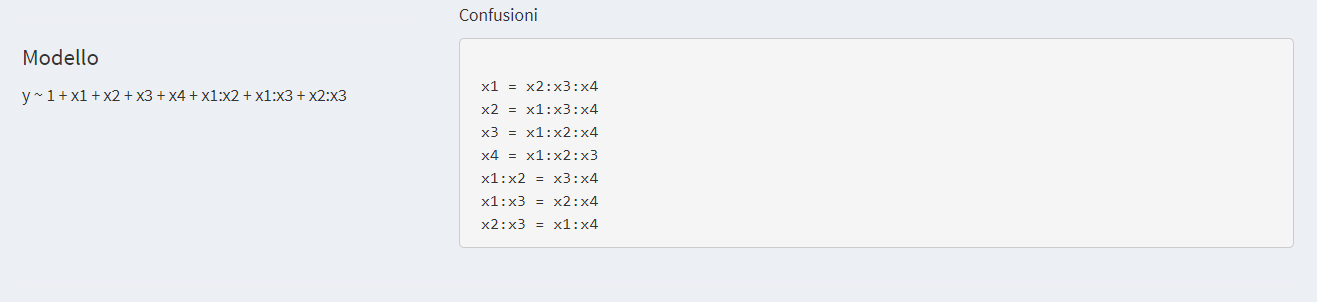
\includegraphics[width=1\linewidth]{Immagini/Fraz/05_esempio2} 

}

\caption{Modello e condusioni del frazionario di  $2_{IV}^{4-1}$}\label{fig:fz5}
\end{figure}

Il disegno è di risoluzione \(IV\) quindi, come si vede in Figura \ref{fig:fz5}, abbiamo ``confusione'' tra i termini lineari e le interazioni di ordine 3 e tra le coppie di interazioni di ordine 2.

Vengono quindi eseguiti, in ordine casuale, gli 8 esperimenti ottenendo per la risposta \emph{Resa} i seguenti valori, Tabella \ref{tab:fzpianorisp}

\begin{table}

\caption{\label{tab:fzpianorisp}Piano sperimentale $2_{IV}^{4-1}$ con risposte}
\centering
\begin{tabular}[t]{ccccc}
\toprule
vol. solvente & t. centrifuga & forza ionica & t. estrazione & Resa\\
\midrule
10 & 5 & 1 & 1 & 17\\
40 & 5 & 1 & 5 & 37.9\\
10 & 20 & 1 & 5 & 17\\
40 & 20 & 1 & 1 & 24.6\\
10 & 5 & 5 & 5 & 28.4\\
\addlinespace
40 & 5 & 5 & 1 & 22.7\\
10 & 20 & 5 & 1 & 30.3\\
40 & 20 & 5 & 5 & 36.3\\
\bottomrule
\end{tabular}
\end{table}

Inserendo nell'applicativo gli 8 valori della \emph{Resa} ottenuti (in ordine come in Tabella \ref{tab:fzpianorisp}, otteniamo la stima puntuale dei parametri Figura \ref{fig:fz6} e il relativo grafico Figura \ref{fig:fz7}.

\begin{figure}[ht]

{\centering 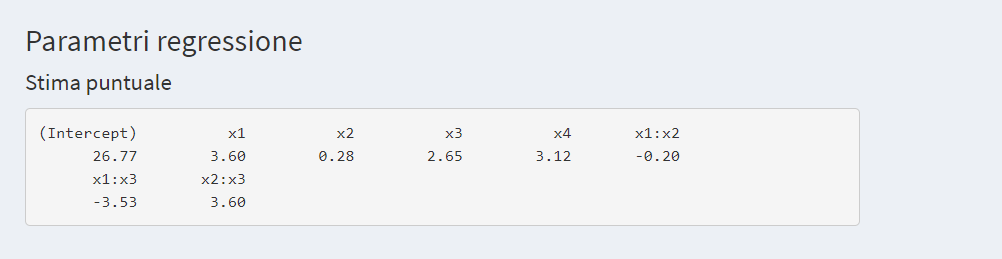
\includegraphics[width=1\linewidth]{Immagini/Fraz/06_parametri} 

}

\caption{Stima puntuale dei parametri}\label{fig:fz6}
\end{figure}

\begin{figure}[ht]

{\centering 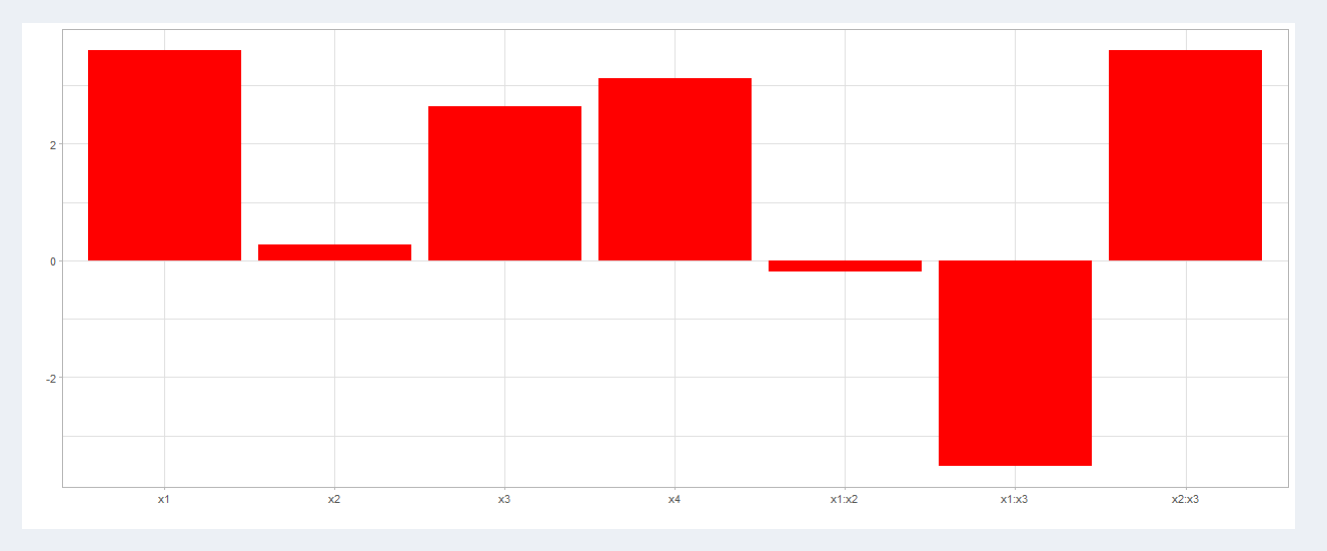
\includegraphics[width=1\linewidth]{Immagini/Fraz/07_graf_parametri} 

}

\caption{Grafico dell stima puntuale dei parametri}\label{fig:fz7}
\end{figure}

Ricordando le ``confusioni'' Figura \ref{fig:fz5} e che il disegno è di risoluzione \(IV\) abbiamo che il termini lineari sono ``confusi'' con le interazioni di ordine 3, possiamo quindi supporre che i valori dei parametri \(x_1,x_2,x_3\) e \(x_4\) si riferiscano ai termini linerari mentre rimangono le ``confusioni'' a coppie per le interazioni di ordine 2.\\
Il modello risulta quindi
\[
y=26.77+3.60x_1+0.28x_2+2.65x_3+3.12x_4-0.2(x_1x_2+x_3x_4)-3.53(x_1x_3+x_2x_4)+3.60(x_1x_4+x_2x_3)
\]

Il fattore \(x_2\) ha coefficiente piccolo e non sembra importante, mentre gli altri tre termini lineari lo sono sicuramente.\\
Quindi si può sostenere l'ipotesi che le interazioni confuse siano dovute ai termini diversi da \(x_2\).\\
Questa osservazione è di fatto risultata coerente con il dato sperimentale osservato secondo cui il tempo di centrifuga non ha alcun effetto sulla resa di estrazione perché il livello più basso scelto è già più che sufficiente per rompere l'emulsione creata dopo la miscelazione delle fasi del solvente di estrazione e del campione.
Tali conclusioni sono confermate dal piano \(2^4\) poi condotto a termine.

Il modello finale semplificato quindi è

\[
y=26.77+3.60x_1+2.65x_3+3.12x_4-0.2x_3x_4-3.53x_1x_3+3.60x_1x_4
\]

Per convalidare il modello sono state eseguite misure indipendenti nel punto test \((1-1,-1,-1,-1)\). Inserendo le rese osservate \(17.2,16.9,17.0,16.8\) nell'apposita casella dell'applicativo si ottiene Figura \ref{fig:fz8}

\begin{figure}[ht]

{\centering 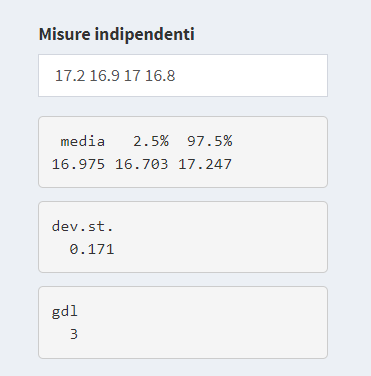
\includegraphics[width=1\linewidth]{Immagini/Fraz/08_mis_ind} 

}

\caption{Misure indipendenti nel punto test}\label{fig:fz8}
\end{figure}

La risposta predetta nel punto test e gli estremi dell'intervallo di confidenza costruito con la stima di \(\sigma\) ottenuta con le 4 misure indipendenti sono dati in Figura \ref{fig:fz9}.

\begin{figure}[ht]

{\centering 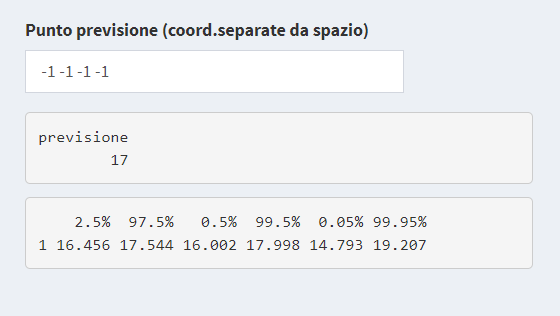
\includegraphics[width=1\linewidth]{Immagini/Fraz/09_prev} 

}

\caption{Previsione nel punto test e estremi dell'intervallo di confidenza}\label{fig:fz9}
\end{figure}

Il modello è convalidato statisticamente e può quindi essere usato per esplorare in modo attendibile il dominio delle risposte, Figura \ref{fig:fz10}

\begin{figure}[ht]

{\centering 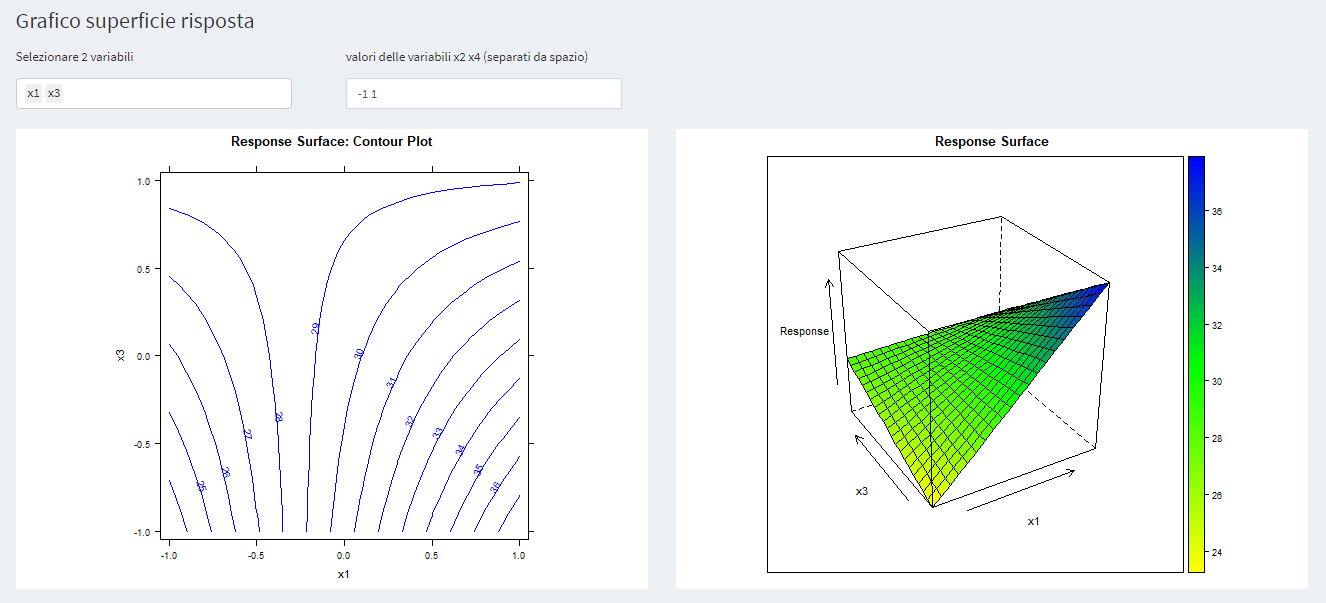
\includegraphics[width=1\linewidth]{Immagini/Fraz/10_sup_risp} 

}

\caption{Grafico della superficie di risposta}\label{fig:fz10}
\end{figure}

\hypertarget{plackett-burman}{%
\chapter{Plackett Burman}\label{plackett-burman}}

I disegni frazionari \(2_{III}^{k-p}\) di risoluzione \(III\) sono usati prevalentemente per condurre studi di screening e di robustezza. Il numero di esperimenti di un qualsiasi piano fattoriale frazionario è comunque uguale ad un numero di esperimenti esponenziale \(2^n\): 8, 16, 32, \ldots{} .
Plackett e Burman nel 1946 hanno introdotto una classe di disegni fattoriali a \(2\) livelli ortogonali che permettono di condurre lo screening di \(n-1\) fattori prevedendo lo svolgimento di un numero \(n=4m\) di esperimenti (4, 8, 12, 16, 20, 24, \ldots), in modo tale da offrire le opzioni per colmare i vuoti esistenti ad esempio tra piani di 8 e 16, oppure di 16 e 32 esperimenti.\\
Nel caso in cui \(n\) sia anche una potenza di \(2\) (4, 8, 16, \ldots), il disegno di PB corrispondente è un particolare disegno frazionario di risoluzione \(III\).

La matrice sperimentale di questi disegni si costruisce seguendo un procedimento iterativo in cui, data la prima riga della matrice (vedi Tabella \ref{tab:PBAlg} di lunghezza \(n-1\), si generano le righe successive per permutazione circolare di questa riga (ogni riga ha al primo posto l'elemento che era all'ultimo posto della riga superiore e agli altri \(i=2,\dots, n-1\) l'elemento di posto \(i-1\) della riga superiore; in totale in questo modo si scrivono \(n-1\) righe, compresa la prima riga data, e a queste si aggiunge una ultima riga composta da solo \(-1\).

\begin{longtable}[]{@{}lrrrrrrrrrrrrrrrrrrr@{}}
\caption{\label{tab:PBAlg}}\tabularnewline
\toprule
n & & & & & & & & & & & & & & & & & & &\tabularnewline
\midrule
\endfirsthead
\toprule
n & & & & & & & & & & & & & & & & & & &\tabularnewline
\midrule
\endhead
4 & 1 & 1 & -1 & & & & & & & & & & & & & & & &\tabularnewline
8 & 1 & 1 & 1 & -1 & 1 & -1 & -1 & & & & & & & & & & & &\tabularnewline
12 & 1 & 1 & -1 & 1 & 1 & 1 & -1 & -1 & -1 & 1 & -1 & & & & & & & &\tabularnewline
16 & 1 & 1 & 1 & 1 & -1 & 1 & -1 & 1 & 1 & -1 & -1 & 1 & -1 & -1 & -1 & & & &\tabularnewline
20 & 1 & 1 & -1 & -1 & 1 & 1 & 1 & 1 & -1 & 1 & -1 & 1 & -1 & -1 & -1 & -1 & 1 & 1 & -1\tabularnewline
\(\cdots\) & & & & & & & & & & & & & & & & & & &\tabularnewline
\bottomrule
\end{longtable}

Vediamo ad esempio la costruzione della matrice per \(n=4.\) La prima riga della matrice, vedi Tabella \ref{tab:PBAlg}, è:\\
\begin{equation*}
    1 \qquad 1 \qquad -1.
\end{equation*}
Generiamo le altre righe \(2\) righe per permutazione circolare e aggiungiamo la quarta riga costituita da \(-1\).

\begin{longtable}[]{@{}crrr@{}}
\caption{Plackett Burman con 4 esperimenti}\tabularnewline
\toprule
\begin{minipage}[b]{0.22\columnwidth}\centering
\strut
\end{minipage} & \begin{minipage}[b]{0.22\columnwidth}\raggedleft
\(\bf{X_1}\)\strut
\end{minipage} & \begin{minipage}[b]{0.22\columnwidth}\raggedleft
\(\bf{X_2}\)\strut
\end{minipage} & \begin{minipage}[b]{0.22\columnwidth}\raggedleft
\(\bf{X_3}\)\strut
\end{minipage}\tabularnewline
\midrule
\endfirsthead
\toprule
\begin{minipage}[b]{0.22\columnwidth}\centering
\strut
\end{minipage} & \begin{minipage}[b]{0.22\columnwidth}\raggedleft
\(\bf{X_1}\)\strut
\end{minipage} & \begin{minipage}[b]{0.22\columnwidth}\raggedleft
\(\bf{X_2}\)\strut
\end{minipage} & \begin{minipage}[b]{0.22\columnwidth}\raggedleft
\(\bf{X_3}\)\strut
\end{minipage}\tabularnewline
\midrule
\endhead
\begin{minipage}[t]{0.22\columnwidth}\centering
1\strut
\end{minipage} & \begin{minipage}[t]{0.22\columnwidth}\raggedleft
1\strut
\end{minipage} & \begin{minipage}[t]{0.22\columnwidth}\raggedleft
1\strut
\end{minipage} & \begin{minipage}[t]{0.22\columnwidth}\raggedleft
-1\strut
\end{minipage}\tabularnewline
\begin{minipage}[t]{0.22\columnwidth}\centering
2\strut
\end{minipage} & \begin{minipage}[t]{0.22\columnwidth}\raggedleft
-1\strut
\end{minipage} & \begin{minipage}[t]{0.22\columnwidth}\raggedleft
1\strut
\end{minipage} & \begin{minipage}[t]{0.22\columnwidth}\raggedleft
1\strut
\end{minipage}\tabularnewline
\begin{minipage}[t]{0.22\columnwidth}\centering
3\strut
\end{minipage} & \begin{minipage}[t]{0.22\columnwidth}\raggedleft
1\strut
\end{minipage} & \begin{minipage}[t]{0.22\columnwidth}\raggedleft
-1\strut
\end{minipage} & \begin{minipage}[t]{0.22\columnwidth}\raggedleft
1\strut
\end{minipage}\tabularnewline
\begin{minipage}[t]{0.22\columnwidth}\centering
4\strut
\end{minipage} & \begin{minipage}[t]{0.22\columnwidth}\raggedleft
-1\strut
\end{minipage} & \begin{minipage}[t]{0.22\columnwidth}\raggedleft
-1\strut
\end{minipage} & \begin{minipage}[t]{0.22\columnwidth}\raggedleft
-1\strut
\end{minipage}\tabularnewline
\bottomrule
\end{longtable}

Il modello associato a questi disegni tiene conto di tutti i fattori lineari
\begin{equation*}
     y_i=\beta_0+\beta_1x_{i1}+\cdots+\beta_{n-1}x_{i,n-1}+\epsilon_i, \qquad i=1,\dots,n,
\end{equation*}
la matrice del modello é uguale alla matrice sperimentale a cui va aggiunta una prima colonna di tutti \(1\). Abbiamo per lo stimatore \(b=X^{-1}Y\)
\begin{equation*}
    Cov(b)=\frac{\sigma^2}{n}I_{n},
\end{equation*}
abbiamo cioè
\begin{equation*}
    Var(b)=\frac{\sigma^2}{n}, \qquad j=1,\dots,n
\end{equation*}
e
\begin{equation*}
    Corr(b_i,b_j)=0, \qquad i\neq j.
\end{equation*}

Nell'applicativo, selezionando il numero di fattori da studiare, viene proposto il disegno di Plackett-Burman con con un numero di esperimenti pari al minimo multiplo di 4 maggione del numero del numero di fattori, Figura \ref{fig:pb1}.

\begin{figure}[ht]

{\centering 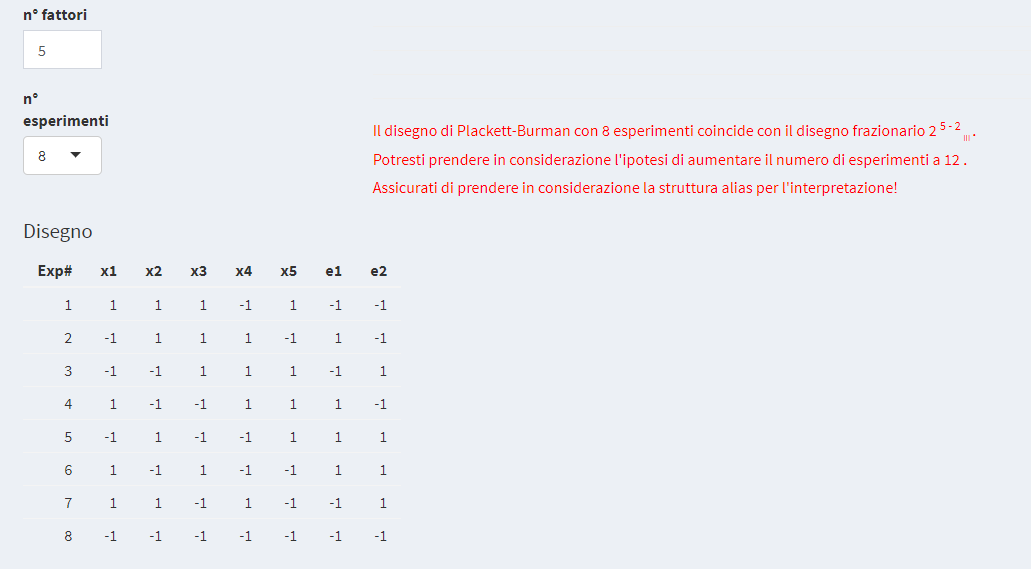
\includegraphics[width=1\linewidth]{Immagini/PB/01_dis} 

}

\caption{Disegno di Plackett-Burman per 5 fattori}\label{fig:pb1}
\end{figure}

Si noti che le prime 5 colonne sono ``occupate'' dai 5 fattori in analisi indicate con \(x_1, \dots,x_5\) mentre vengono indicate con \(e_1,e_2\) le 2 colonne rimanenti. Queste sono 2 variabili cosiddette \emph{dummy} (variabili fittizie) che possono essere utili per stabilire la significatività dei fattori in studio. Si vedano al riguardo gli esempi nel seguito.

I disegni di Plackett-Burman sono disegni di risoluzione \(III\), nel senso che le interazioni sono confuse con i termini lineari. Nel caso in cui il numero di esperimenti \(n\) sia una potenza di \(2\), come abbiamo già detto, il disegno di Plackett-Burmann è un particolare disegno frazionario di risoluzione \(III\) e quindi i termini lineari sono ``completamente confusi'' con le interazioni (si veda la sezione dedicata ai disegni frazionari). Nei casi in cui \(n\) non è una potenza di \(2\), per determinare le relazioni ``confuse'' si considerano la matrice \(X_1\) del modello Tabella \ref{tab:matrmod}\newpage

\begin{table}

\caption{\label{tab:matrmod}Matrice del modello}
\centering
\begin{tabular}[t]{rrrrrrrr}
\toprule
Int. & x1 & x2 & x3 & x4 & x5 & e1 & e2\\
\midrule
1 & 1 & 1 & 1 & -1 & 1 & -1 & -1\\
1 & -1 & 1 & 1 & 1 & -1 & 1 & -1\\
1 & -1 & -1 & 1 & 1 & 1 & -1 & 1\\
1 & 1 & -1 & -1 & 1 & 1 & 1 & -1\\
1 & -1 & 1 & -1 & -1 & 1 & 1 & 1\\
\addlinespace
1 & 1 & -1 & 1 & -1 & -1 & 1 & 1\\
1 & 1 & 1 & -1 & 1 & -1 & -1 & 1\\
1 & -1 & -1 & -1 & -1 & -1 & -1 & -1\\
\bottomrule
\end{tabular}
\end{table}

e la matrice \(X_2\) dei termini (interazioni) confusi Tabella \ref{tab:pbmatrconf}

\begin{table}

\caption{\label{tab:pbmatrconf}Matrice delle interazioni confuse}
\centering
\begin{tabular}[t]{rrrrrrlrrrrrr}
\toprule
x1x2 & x1x3 & x1x4 & x1x5 & x1e1 & x1e2 & ... & x4x5 & x4e1 & x4e2 & x5e1 & x5e2 & e1e2\\
\midrule
1 & 1 & -1 & 1 & -1 & -1 &  & -1 & 1 & 1 & -1 & -1 & 1\\
-1 & -1 & -1 & 1 & -1 & 1 &  & -1 & 1 & -1 & -1 & 1 & -1\\
1 & -1 & -1 & -1 & 1 & -1 &  & 1 & -1 & 1 & -1 & 1 & -1\\
-1 & -1 & 1 & 1 & 1 & -1 &  & 1 & 1 & -1 & 1 & -1 & -1\\
-1 & 1 & 1 & -1 & -1 & -1 &  & -1 & -1 & -1 & 1 & 1 & 1\\
\addlinespace
-1 & 1 & -1 & -1 & 1 & 1 &  & 1 & -1 & -1 & -1 & -1 & 1\\
1 & -1 & 1 & -1 & -1 & 1 &  & -1 & -1 & 1 & 1 & -1 & -1\\
1 & 1 & 1 & 1 & 1 & 1 &  & 1 & 1 & 1 & 1 & 1 & 1\\
\bottomrule
\end{tabular}
\end{table}

La matrice A, spesso indicata anche con il nome di ``\emph{alias matrix}'', o matrice di confusione, è definita dalla relazione algebrica
\[
A=(X_1^tX_1)^{-1}(X_1^tX_2)
\]
La matrice A ha tante righe quanti sono i termini del modello (in questo caso 8: intercetta, 5 fattori e due variabili fittizie) e tante colonne quante sono le interazioni possibili (in questo caso 21 interazioni a due termini), e si chiama matrice di confusione.\\
In Figura \ref{fig:pb2} è illustrata la matrice di confusione relativa al modello di Plackett-Burman per 5 fattori di cui è data la matrice in Figura \ref{fig:pb1}. Nella matrice di confusione, in ogni riga si può leggere la ``confusione'' di ogni termine lineare con le interazioni di due termini.

\begin{figure}[ht]

{\centering 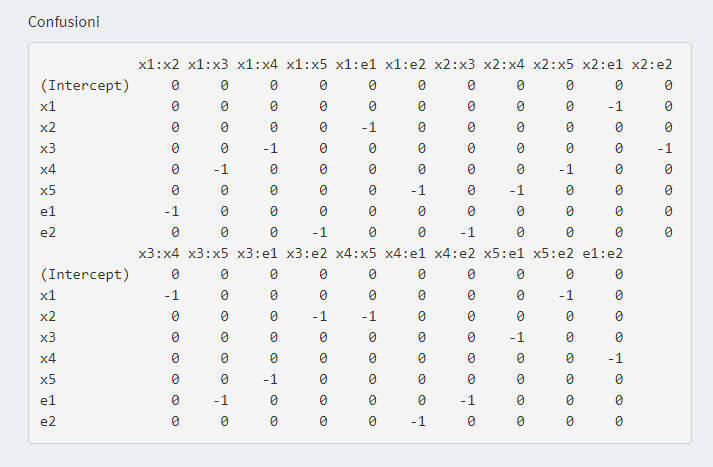
\includegraphics[width=1\linewidth]{Immagini/PB/02_matr_conf} 

}

\caption{Matrice di confusione}\label{fig:pb2}
\end{figure}

Il caso in esame è un frazionario \(2^{5-2}_{III}\) e le confusioni, come ci aspettiamo, sono ``totali'' o ``complete'': ciò significa che ogni interazione è ``confusa'' con un solo termine lineare. Si noti che nella matrice di confusione di questo modello appaiono solo segni 0 o -1.

Scegliendo 12 esperimenti, la matrice di confusione è quella data in Figura \ref{fig:pb3}

\begin{figure}[ht]

{\centering 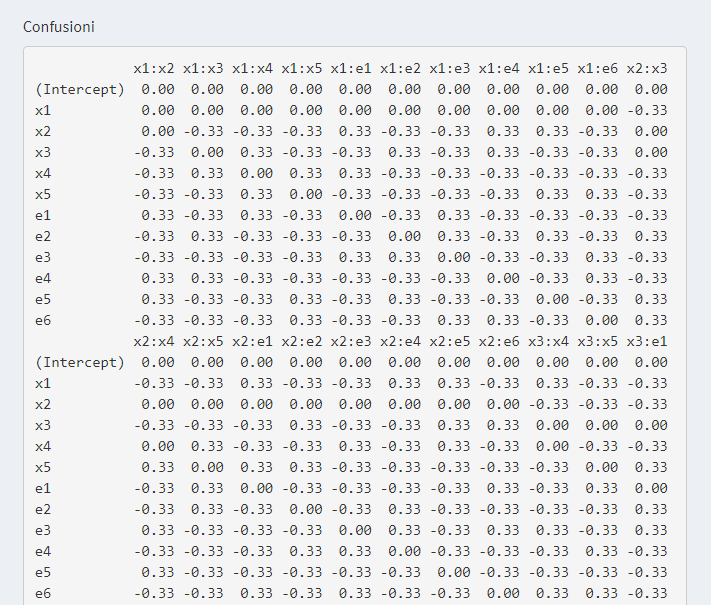
\includegraphics[width=1\linewidth]{Immagini/PB/03_matr_conf_12} 

}

\caption{Parte della matrice di confusione di un disegno di Plackett-Burman con 12 esperimenti}\label{fig:pb3}
\end{figure}

In questo caso le ``confusioni'' sono ``parziali'', cioè le interazioni si confondono ``parzialmente'' con più termini lineari. Questo ci permette di stimare le interazioni con l'analisi di regressione. Possiamo sostituire gli effetti lineari meno significativi con le interazioni più importanti. Per determinare le interazioni più rilevanti si moltiplicano per un'interazione fissata le confusioni con i termini lineari più grandi per il segno del coefficiente del termine lineare e se ne fa la somma. Nell'applicativo è proposto il grafico delle confusioni (Plot alias) in cui è rappresentata visivamente tale somma Figura \ref{fig:pb4}

Per meglio chiarire quanto finora detto detto facciamo 2 esempi numerici.

\hypertarget{esempio-confusioni-1}{%
\section{Esempio: confusioni}\label{esempio-confusioni-1}}

Come fatto nel caso del disegno frazionario, per capire le ``confusioni'' in un disegno di Plackett-Burman, consideriamo un modello teorico di un ipotetico fenomeno in esame
\[
y=x_1+5x_2-3x_3+15x_4-15x_1x_3+\epsilon
\]
e supponiamo che si vogliano analizzare gli effetti di 5 fattori
\[
x_1,x_2,x_3,x_4,x_5
\]
perché dall'analisi preliminare del problema è emerso che potrebbero essere importanti nell'influenzare la risposta.

Con 5 fattori il primo disegno di Plackett-Burman ``utile'' è quello che prevede di eseguire 8 esperimenti Tabella \ref{tab:pbes1}

\begin{table}

\caption{\label{tab:pbes1}Disegno di Plackett-Burman con 8 esperimenti con risposte costruite dal modello supposto
            $y=x_1+5x_2-3x_3+15x_4-15x_1x_3+\epsilon$ }
\centering
\begin{tabular}[t]{rrrrrrrr}
\toprule
x1 & x2 & x3 & x4 & x5 & e1 & e2 & y\\
\midrule
1 & 1 & 1 & -1 & 1 & -1 & -1 & 2.66\\
-1 & 1 & 1 & 1 & -1 & 1 & -1 & 1.26\\
-1 & -1 & 1 & 1 & 1 & -1 & 1 & -9.53\\
1 & -1 & -1 & 1 & 1 & 1 & -1 & -0.81\\
-1 & 1 & -1 & -1 & 1 & 1 & 1 & 5.62\\
\addlinespace
1 & -1 & 1 & -1 & -1 & 1 & 1 & -9.10\\
1 & 1 & -1 & 1 & -1 & -1 & 1 & 8.56\\
-1 & -1 & -1 & -1 & -1 & -1 & -1 & -3.04\\
\bottomrule
\end{tabular}
\end{table}

E' un disegno fattoriale frazionario a due livelli con risoluzione \(III\). I termini lineari sono confusi con i termini di interazione di ordine 2. Si noti il valore \(-1\) nella matrice delle confusioni Figura \ref{fig:pb6}

\begin{figure}[ht]

{\centering 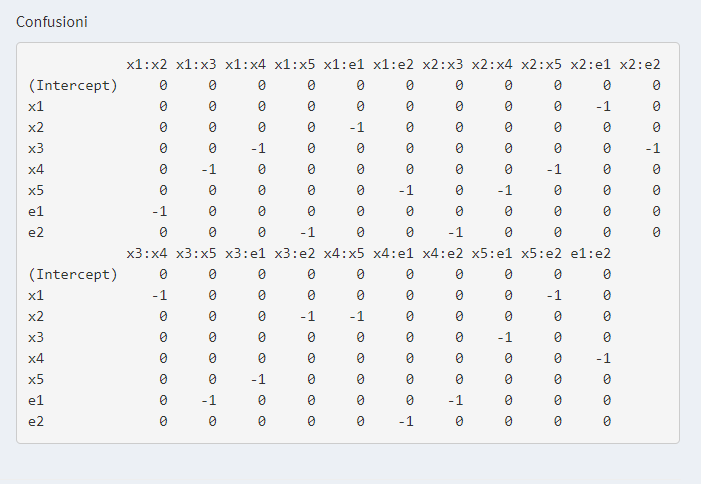
\includegraphics[width=1\linewidth]{Immagini/PB/06_confusioni8} 

}

\caption{Matrice delle confusioni di un pb con 8 esperimenti}\label{fig:pb6}
\end{figure}

Il grafico dei coefficienti è dato da Figura \ref{fig:pb7}

\begin{figure}[ht]

{\centering 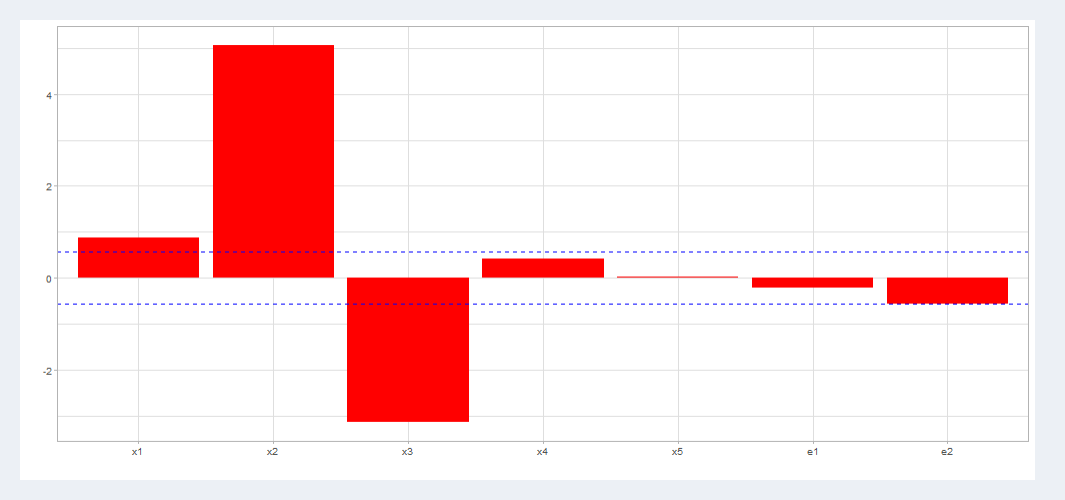
\includegraphics[width=1\linewidth]{Immagini/PB/07_coeff8} 

}

\caption{Grafico dei coefficienti del pb con 8 esperiemnti}\label{fig:pb7}
\end{figure}
\newpage

Se a priori non possiamo escludere nessuna interazione di ordine 2, potrebbe accadere che la non significatività dei termini \(x_4\) e \(x_5\) sia dovuta al fatto che si annullino con le interazioni di ordine 2 con cui sono confusi. Ad esempio, \(x_4\) potrebbe annullarsi con \(x_1x_3\) (\(x_4\) si confonde con \(-x_1x_3\) e, se i coefficienti di questi termini hanno valore numerico simile, come nel nostro esempio, si annullano).\\
Anche per le dummy bisogna fare attenzione e essere sicuri che non appaiano importanti perchè ``rappresentano'' in realtà una interazione confusa con esse.

Non possiamo sapere quindi se la significatività che osserviamo per alcuni termini è autentica, ossia dovuta realmente al fattore stesso, oppure derivi dalle interazioni confuse con ciascun termine. In questi casi, è solo la conoscenza tecnica del problema chimico (o fisico o ingegneristico) che può aiutare a definire la reale importanza dei diversi termini e a giungere alla conclusione di escludere alcune interazioni (perché ad esempio prive di senso fisico o impossibili tecnicamente).

Se a priori invece non si può escludere nessuna interazione, si può prendere in considerazione il piano sperimentale di Plackett-Burman successivo, ossia quello che prevede 12 esperimenti. Questo numero di prove è comunque inferiore a quello del fattoriale frazionario corrispondente che è il \(2^{5-1}_V\)), e conta quindi 16 esperimenti, Tabella \ref{tab:pb12}
\newpage

\begin{table}

\caption{\label{tab:pb12}Disegno di Plackett-Burman con 12 esperimenti con risposte costruite dal modello ipotizzato
            $y=x_1+5x_2-3x_3+15x_4-15x_1x_3+\epsilon$ }
\centering
\begin{tabular}[t]{rrrrrrrrrrrr}
\toprule
x1 & x2 & x3 & x4 & x5 & e1 & e2 & e3 & e4 & e5 & e6 & y\\
\midrule
1 & 1 & -1 & 1 & 1 & 1 & -1 & -1 & -1 & 1 & -1 & 10.41\\
-1 & 1 & 1 & -1 & 1 & 1 & 1 & -1 & -1 & -1 & 1 & -28.31\\
1 & -1 & 1 & 1 & -1 & 1 & 1 & 1 & -1 & -1 & -1 & 24.41\\
-1 & 1 & -1 & 1 & 1 & -1 & 1 & 1 & 1 & -1 & -1 & 36.73\\
-1 & -1 & 1 & -1 & 1 & 1 & -1 & 1 & 1 & 1 & -1 & -38.92\\
\addlinespace
-1 & -1 & -1 & 1 & -1 & 1 & 1 & -1 & 1 & 1 & 1 & 26.56\\
1 & -1 & -1 & -1 & 1 & -1 & 1 & 1 & -1 & 1 & 1 & -29.71\\
1 & 1 & -1 & -1 & -1 & 1 & -1 & 1 & 1 & -1 & 1 & -20.04\\
1 & 1 & 1 & -1 & -1 & -1 & 1 & -1 & 1 & 1 & -1 & 3.18\\
-1 & 1 & 1 & 1 & -1 & -1 & -1 & 1 & -1 & 1 & 1 & 1.26\\
\addlinespace
1 & -1 & 1 & 1 & 1 & -1 & -1 & -1 & 1 & -1 & 1 & 21.81\\
-1 & -1 & -1 & -1 & -1 & -1 & -1 & -1 & -1 & -1 & -1 & -3.04\\
\bottomrule
\end{tabular}
\end{table}

Il grafico dei coefficienti è dato da Figura \ref{fig:pb8}

\begin{figure}[ht]

{\centering 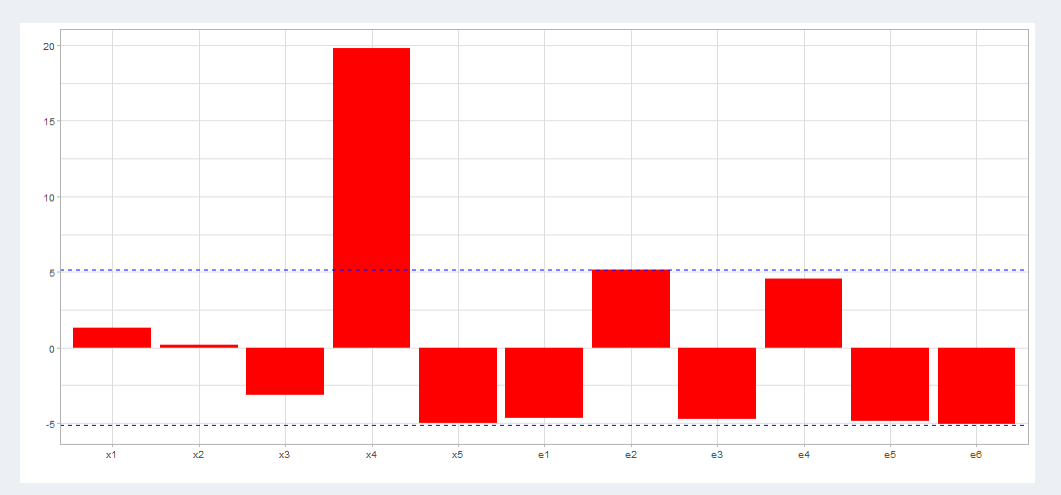
\includegraphics[width=1\linewidth]{Immagini/PB/08_coeff12} 

}

\caption{Grafico dei coefficienti del piano di Plackett-Burman con 12 esperimenti}\label{fig:pb8}
\end{figure}

Quando si applicano piani di Plackett-Burman quindi è molto importante prestare la massima attenzione alla significatività dei fattori e alle possibili interazioni confuse con essi. Questo vale a maggior ragione per le variabili dummy che, come visto, possono essere confuse con le interazioni coppie al pari di qualsiasi altro fattore compreso nel piano degli esperimenti.\\
Nel caso di un piano sperimentale di 12 esperimenti,le confusioni sono parziali. Si noti il valore \(-0.33\) nella matrice delle confusioni Figura \ref{fig:pb3}. Tale valore permette di stimare le interazioni con l'analisi di regressione. Possiamo sostituire gli effetti lineari meno importanti con le interazioni più significative.
\newpage
Per determinare le interazioni più significative, si moltiplicano queste per una interazione fissata, si moltiplicano le confusioni con i termini lineari più importanti per il segno del coefficiente del termine lineare e se ne fa la somma Figura \ref{fig:pb9}.

\begin{figure}[ht]

{\centering 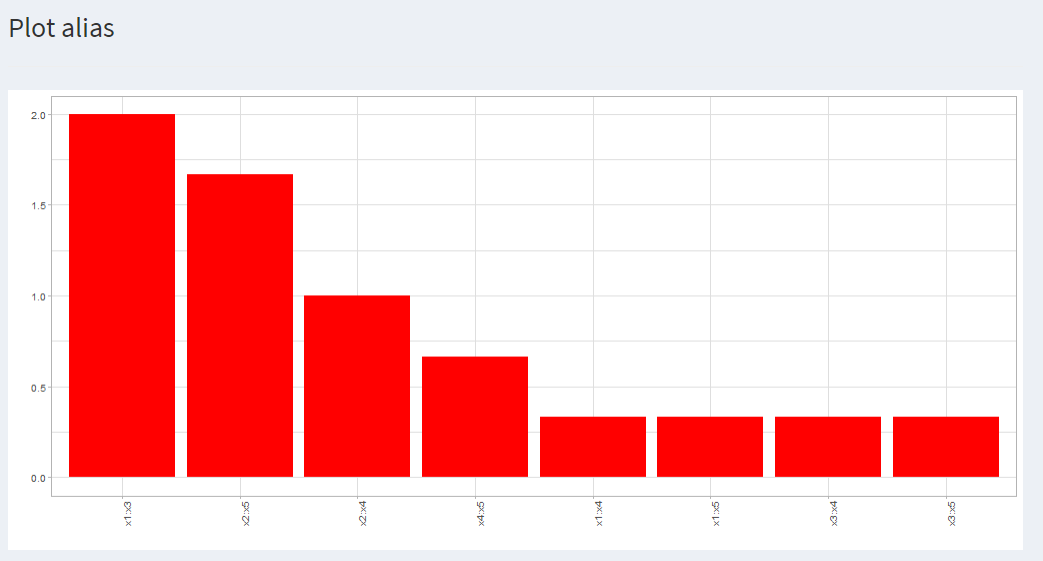
\includegraphics[width=1\linewidth]{Immagini/PB/09_alias12} 

}

\caption{Grafico dei coefficienti del pb con 12 esperimenti}\label{fig:pb9}
\end{figure}

Con l'applicativo possiamo innanzitutto scaricare un disegno di Plackett-Burman con 12 esperimenti e quindi ricaricare il file salvato nel menù \emph{Piano Personalizzato} (se si preferisce si può anche importare il disegno con copia/incolla). Vedi Figura \ref{fig:pb10}

\begin{figure}[ht]

{\centering 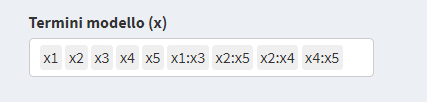
\includegraphics[width=1\linewidth]{Immagini/PB/10_pp1} 

}

\caption{Selezione delle variabili}\label{fig:pb10}
\end{figure}

Una volta importato il datset selezioniamo i termini del modello che vogliamo studiare. Nel nostro caso ad esempio possiamo considerare i 5 termini lineari e le 4 interazioni \(x_1x_3,x_2x_5,x_2x_4,x_4x_5\) che hanno maggiore probabilità di essere significative, vedi Figura \ref{fig:pb9}.\\
Inserendo le 12 risposte nell'opportuno riquadro otteniamo il seguente grafico dei coefficienti Figura \ref{fig:pb11}.

\begin{figure}[ht]

{\centering 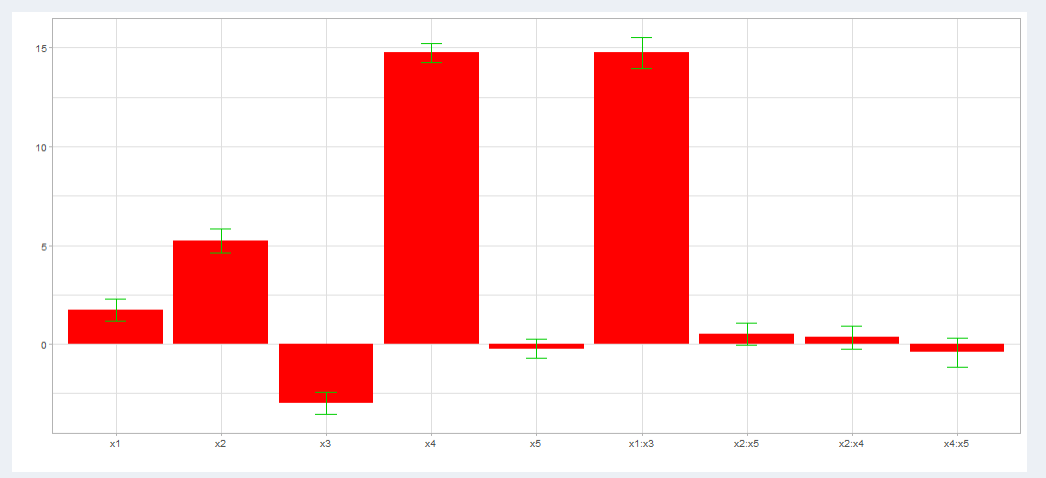
\includegraphics[width=1\linewidth]{Immagini/PB/11_pp2} 

}

\caption{Selezione delle variabili}\label{fig:pb11}
\end{figure}

Tale grafico evidenzia la significatività sia di \(x_4\) che dell'interazione \(x_1x_3\) che non riuscivamo a distinguere poiché questi termini, a causa delle confusioni, si annullavano a vicenda.

\hypertarget{esempio-elvitegravir}{%
\section{Esempio Elvitegravir}\label{esempio-elvitegravir}}

Il problema è lo sviluppo di un metodo semplice per l'isolamento di un principio attivo da plasma umano preliminare all'analisi HPLC-ESI/MS/MS. La risposta è la sensibilità S/N, che si vuole massimalizzzare.\\
Tra tutti i fattori considerati si è deciso di considerare i 5 fattori:

\begin{itemize}
\tightlist
\item
  x1: Solvente (agente precipitante)
\item
  x2: Volume di plasma (µL)
\item
  x3: Volume di solvente (rapp v.campione)
\item
  x4: Tempo miscelazione (sec)
\item
  x5: Temperatura centrifuga (°C)
\end{itemize}

Il dominio sperimentale è definito in Tabella \ref{tab:pbliv1}
\newpage

\begin{table}

\caption{\label{tab:pbliv1}Definizione dei livelli dei 5 fattori}
\centering
\begin{tabular}[t]{lll}
\toprule
Fattori & -1 & +1\\
\midrule
Solvente & ACN & MeOH\\
Plasma & 50 & 200\\
Solvente (vol) & 1:3 & 1:7\\
Miscelazione & 20 & 60\\
Centrifuga & 4 & 25\\
\bottomrule
\end{tabular}
\end{table}

Si sceglie un disegno di Plackett-Burnan con 8 esperimenti. Sono quindi aggiunte al piano sperimentale 2 variabili dummy

\begin{itemize}
\tightlist
\item
  e1: orologio al polso
\item
  e2: canto mentre lavoro
\end{itemize}

I livelli delle 2 variabili fittizie sono dati nella Tabella \ref{tab:dummy1}. Sono 2 variabili che sicuramente non hanno alcuna influenza sulla risposta e che saranno utili quindi per avere un benchmark di significatività (o se si preferisce, una stima della importanza del rumore di fondo casuale nei risultati degli esperimenti).

\begin{table}

\caption{\label{tab:dummy1}Definizione dei livelli dei 2 fattori  dummy}
\centering
\begin{tabular}[t]{lll}
\toprule
Fattori & -1 & +1\\
\midrule
Orologio & sin & dx\\
Canto & si & no\\
\bottomrule
\end{tabular}
\end{table}

Il disegno con le relative risposte è dato in Tabella \ref{tab:pbes2}
\newpage

\begin{table}

\caption{\label{tab:pbes2}Disegno di Plackett-Burman per lo sviluppo del metodo di estrazione di Elvitegravir con risposte}
\centering
\begin{tabular}[t]{rrrrrrrrr}
\toprule
Exp. & x1 & x2 & x3 & x4 & x5 & e1 & e2 & S.N\\
\midrule
1 & 1 & 1 & 1 & -1 & 1 & -1 & -1 & 31795\\
2 & -1 & 1 & 1 & 1 & -1 & 1 & -1 & 33313\\
3 & -1 & -1 & 1 & 1 & 1 & -1 & 1 & 32264\\
4 & 1 & -1 & -1 & 1 & 1 & 1 & -1 & 31559\\
5 & -1 & 1 & -1 & -1 & 1 & 1 & 1 & 35150\\
\addlinespace
6 & 1 & -1 & 1 & -1 & -1 & 1 & 1 & 21201\\
7 & 1 & 1 & -1 & 1 & -1 & -1 & 1 & 32344\\
8 & -1 & -1 & -1 & -1 & -1 & -1 & -1 & 21087\\
\bottomrule
\end{tabular}
\end{table}

\newpage

Inserendo le risposte nell'applicativo ottieniamo la stima dei parametri in Figura \ref{fig:pb5}

\begin{figure}[ht]

{\centering 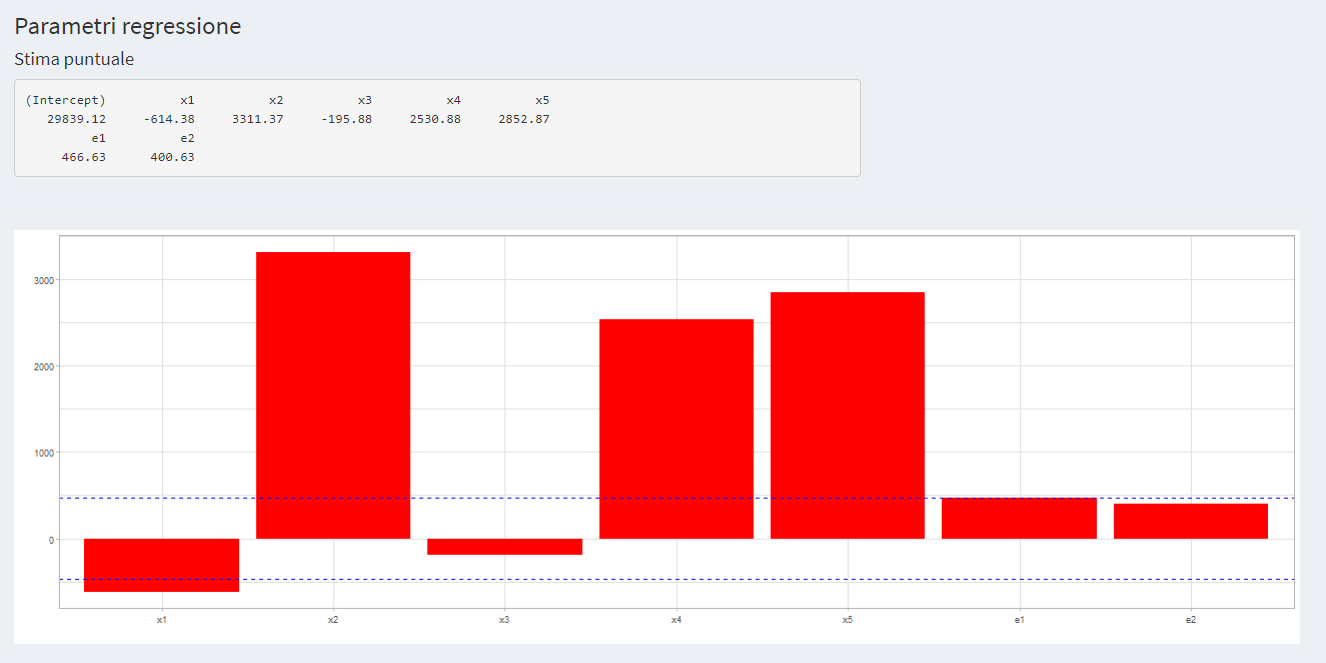
\includegraphics[width=1\linewidth]{Immagini/PB/05_coeff1} 

}

\caption{Stima dei parametri}\label{fig:pb5}
\end{figure}

Come detto, le 2 variabili dummy possono essere usate come benchmark di significatività. Quindi tutti i parametri che in valore assoluto sono minori del valore assoluto dei coefficienti delle 2 variabili dummy possono essere considerati non significativi. In Figura \ref{fig:pb5} sono tracciate 2 linee orizzontali indicanti la fascia di non significatività. La variabile \(x_4\) (Tempo miscelazione, misurata in sec) è non significativa.

Lo studio può continuare raffinando l'indagine con un nuovo piano di esperimenti che prenda in esame solo questi 4 fattori significativi.

\begin{figure}[ht]

{\centering 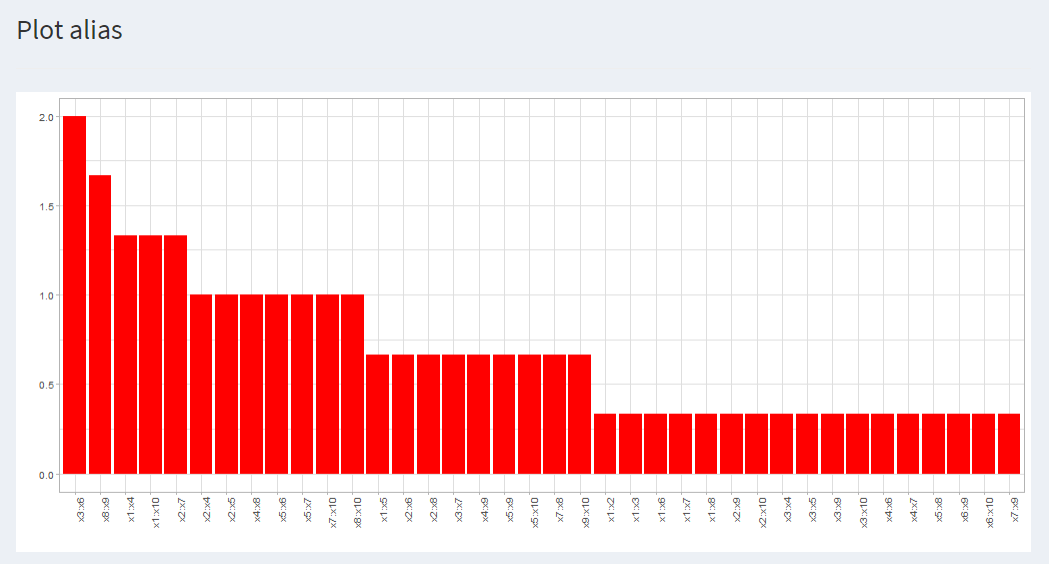
\includegraphics[width=1\linewidth]{Immagini/PB/04_plot_alias} 

}

\caption{Plot alias}\label{fig:pb4}
\end{figure}

\hypertarget{central-composite-design}{%
\chapter{Central Composite Design}\label{central-composite-design}}

I disegni fattoriali completi, frazionari e Plackett-Burman sono utili per lo screening dei fattori e delle loro eventuali interazioni che abbiano effetto su un fenomeno analizzato.\\
In questo capitolo siamo interessati al problema dell'ottimizzazione della variabile risposta nel dominio sperimentale. In termini analitici, per fissare le idee, ciò significa verificare se la risposta sperimentale ha massimi o minimi. Quindi, per gli studi di ottimizzazione, generalmente, bisogna analizzare la forma della superficie di risposta e verificare se essa ha una curvatura.\\
Per superficie di risposta intendiamo la superficie descritta dalla funzione \(f\), funzione teorica che descrive il fenomeno studiato
\[
    y=f(X_1,\dots,X_k),
\]
dove \(X_1,\dots,X_k\) sono i fattori che influenzano il fenomeno studiato. La risposta sarà quindi
\[
    Y=f(X_1,\dots,X_k)+\epsilon,
\]
dove \(\epsilon\) rappresenta l'errore sulla risposta osservata.

Ricordando che, poichè ogni funzione \(f\) passante per un punto \(\underline{x}_0=(x_{01},\dots,x_{0k})\) di \(\mathbb{R}^k\) sufficientemente regolare (ossia differenziabile un numero sufficiente di volte in un intorno di \(\underline{x}_0\)) è approssimabile (formula di Taylor) da un polinomio \(P_m\) di grado \(m\)
\[
    f(\underline{x})=P_m(\underline{x})+R(\underline{x}), \qquad \underline{x} \in \mathbb{R}^k
\]
dove
\[
    \lim_{\underline{x} \to \underline{x}_0}
    \frac{R(\underline{x})}{\|\underline{x}-\underline{x}_0 \|^m}=0,
\]
è sufficiente approssimare la risposta con un modello quadratico (posto \(\underline{x}_0=0\))
\[
     Y=\beta_0+\beta_1 X_1+\cdots +\beta_k X_k +
    \beta_{12}X_1X_2+\cdots+\beta_{k-1, k}X_{k-1}  X_k+
    \beta_{11}X_1^2+\cdots+\beta_{kk}X_k^2+\epsilon 
\]

Si osservi che nell'uso dei disegni fattoriali completi, frazionari e di Plackett-Burman abbiamo approssimato la superficie risposta con un piano descritto dal modello lineare contenente solo gli effetti principali dei fattori e abbiamo analizzato le ``deformazioni'' di questo piano dovute alle interazione tra fattori aggiungendo i termini di interazione a due termini nel modello lineare.

I domini sperimentali considerati in questi disegni non sono adatti ai modelli quadratici in quanto la relativa matrice di informazione non è invertibile, perché le colonne della matrice modello corrispondenti ai termini quadratici coincidono con la colonna \emph{Int.}. Se la matrice di informazione non è invertibile, non esiste matrice di dispersione e non è possibile stimare i coefficienti del modello.

Per ovviare a questo problema Box e Wilson hanno proposto un disegno fattoriale completo a cui vanno aggiunti \(N\) punti centrali e \(2k\) punti stellati, ossia per ogni fattore \(X_j\) consideriamo i punti \((0,\dots,0,a,0,\dots,0)\) e \((0,\dots,0,-a,0,\dots,0)\) lungo l'asse \(X_j\), con \(a>1\). Per ogni fattore sono considerati \(5\) livelli.\\
Otteniamo così un disegno, chiamato disegno composito centrale e indicato con CCD, di \(2^k+2k+N\) punti.\\
Esempio di un CCD per \(k=2,3\) e \(a>1\) è rappresentato in Figura \ref{fig:ccd1}.

\begin{figure}[ht]

{\centering 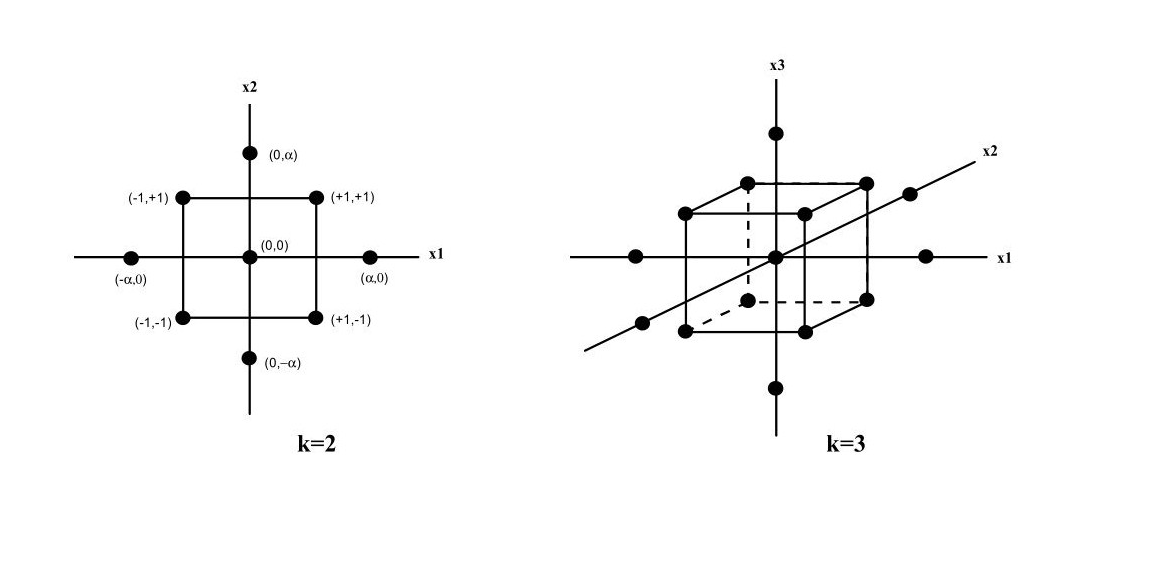
\includegraphics[width=1\linewidth]{Immagini/CCD/01_Rappresentazione} 

}

\caption{Rappresentazione grafica del posizionamento dei punti stella in CCD}\label{fig:ccd1}
\end{figure}

La matrice di tali disegni è data dalla matrice in Tabella \ref{tab:MatrDisCCD}

\begin{longtable}[]{@{}ccccc@{}}
\caption{\label{tab:MatrDisCCD} Matrice disegno composito centrale}\tabularnewline
\toprule
\begin{minipage}[b]{0.17\columnwidth}\centering
\strut
\end{minipage} & \begin{minipage}[b]{0.17\columnwidth}\centering
\(\bf{X_1}\)\strut
\end{minipage} & \begin{minipage}[b]{0.17\columnwidth}\centering
\(\bf{X_2}\)\strut
\end{minipage} & \begin{minipage}[b]{0.17\columnwidth}\centering
\(\cdots\)\strut
\end{minipage} & \begin{minipage}[b]{0.17\columnwidth}\centering
\(\bf{X_k}\)\strut
\end{minipage}\tabularnewline
\midrule
\endfirsthead
\toprule
\begin{minipage}[b]{0.17\columnwidth}\centering
\strut
\end{minipage} & \begin{minipage}[b]{0.17\columnwidth}\centering
\(\bf{X_1}\)\strut
\end{minipage} & \begin{minipage}[b]{0.17\columnwidth}\centering
\(\bf{X_2}\)\strut
\end{minipage} & \begin{minipage}[b]{0.17\columnwidth}\centering
\(\cdots\)\strut
\end{minipage} & \begin{minipage}[b]{0.17\columnwidth}\centering
\(\bf{X_k}\)\strut
\end{minipage}\tabularnewline
\midrule
\endhead
\begin{minipage}[t]{0.17\columnwidth}\centering
1\strut
\end{minipage} & \begin{minipage}[t]{0.17\columnwidth}\centering
-1\strut
\end{minipage} & \begin{minipage}[t]{0.17\columnwidth}\centering
-1\strut
\end{minipage} & \begin{minipage}[t]{0.17\columnwidth}\centering
\(\cdots\)\strut
\end{minipage} & \begin{minipage}[t]{0.17\columnwidth}\centering
-1\strut
\end{minipage}\tabularnewline
\begin{minipage}[t]{0.17\columnwidth}\centering
2\strut
\end{minipage} & \begin{minipage}[t]{0.17\columnwidth}\centering
1\strut
\end{minipage} & \begin{minipage}[t]{0.17\columnwidth}\centering
-1\strut
\end{minipage} & \begin{minipage}[t]{0.17\columnwidth}\centering
\(\cdots\)\strut
\end{minipage} & \begin{minipage}[t]{0.17\columnwidth}\centering
-1\strut
\end{minipage}\tabularnewline
\begin{minipage}[t]{0.17\columnwidth}\centering
3\strut
\end{minipage} & \begin{minipage}[t]{0.17\columnwidth}\centering
-1\strut
\end{minipage} & \begin{minipage}[t]{0.17\columnwidth}\centering
1\strut
\end{minipage} & \begin{minipage}[t]{0.17\columnwidth}\centering
\(\cdots\)\strut
\end{minipage} & \begin{minipage}[t]{0.17\columnwidth}\centering
-1\strut
\end{minipage}\tabularnewline
\begin{minipage}[t]{0.17\columnwidth}\centering
4\strut
\end{minipage} & \begin{minipage}[t]{0.17\columnwidth}\centering
1\strut
\end{minipage} & \begin{minipage}[t]{0.17\columnwidth}\centering
1\strut
\end{minipage} & \begin{minipage}[t]{0.17\columnwidth}\centering
\(\cdots\)\strut
\end{minipage} & \begin{minipage}[t]{0.17\columnwidth}\centering
-1\strut
\end{minipage}\tabularnewline
\begin{minipage}[t]{0.17\columnwidth}\centering
\(\cdot\)\strut
\end{minipage} & \begin{minipage}[t]{0.17\columnwidth}\centering
\(\cdot\)\strut
\end{minipage} & \begin{minipage}[t]{0.17\columnwidth}\centering
\(\cdot\)\strut
\end{minipage} & \begin{minipage}[t]{0.17\columnwidth}\centering
\(\cdots\)\strut
\end{minipage} & \begin{minipage}[t]{0.17\columnwidth}\centering
\(\cdot\)\strut
\end{minipage}\tabularnewline
\begin{minipage}[t]{0.17\columnwidth}\centering
\(\cdot\)\strut
\end{minipage} & \begin{minipage}[t]{0.17\columnwidth}\centering
\(\cdot\)\strut
\end{minipage} & \begin{minipage}[t]{0.17\columnwidth}\centering
\(\cdot\)\strut
\end{minipage} & \begin{minipage}[t]{0.17\columnwidth}\centering
\(\cdots\)\strut
\end{minipage} & \begin{minipage}[t]{0.17\columnwidth}\centering
\(\cdot\)\strut
\end{minipage}\tabularnewline
\begin{minipage}[t]{0.17\columnwidth}\centering
\(\cdot\)\strut
\end{minipage} & \begin{minipage}[t]{0.17\columnwidth}\centering
\(\cdot\)\strut
\end{minipage} & \begin{minipage}[t]{0.17\columnwidth}\centering
\(\cdot\)\strut
\end{minipage} & \begin{minipage}[t]{0.17\columnwidth}\centering
\(\cdots\)\strut
\end{minipage} & \begin{minipage}[t]{0.17\columnwidth}\centering
\(\cdot\)\strut
\end{minipage}\tabularnewline
\begin{minipage}[t]{0.17\columnwidth}\centering
\(2^k\)\strut
\end{minipage} & \begin{minipage}[t]{0.17\columnwidth}\centering
1\strut
\end{minipage} & \begin{minipage}[t]{0.17\columnwidth}\centering
1\strut
\end{minipage} & \begin{minipage}[t]{0.17\columnwidth}\centering
\(\cdots\)\strut
\end{minipage} & \begin{minipage}[t]{0.17\columnwidth}\centering
1\strut
\end{minipage}\tabularnewline
\begin{minipage}[t]{0.17\columnwidth}\centering
\strut
\end{minipage} & \begin{minipage}[t]{0.17\columnwidth}\centering
\strut
\end{minipage} & \begin{minipage}[t]{0.17\columnwidth}\centering
\strut
\end{minipage} & \begin{minipage}[t]{0.17\columnwidth}\centering
\strut
\end{minipage} & \begin{minipage}[t]{0.17\columnwidth}\centering
\strut
\end{minipage}\tabularnewline
\begin{minipage}[t]{0.17\columnwidth}\centering
-1\strut
\end{minipage} & \begin{minipage}[t]{0.17\columnwidth}\centering
-a\strut
\end{minipage} & \begin{minipage}[t]{0.17\columnwidth}\centering
0\strut
\end{minipage} & \begin{minipage}[t]{0.17\columnwidth}\centering
\(\cdots\)\strut
\end{minipage} & \begin{minipage}[t]{0.17\columnwidth}\centering
1\strut
\end{minipage}\tabularnewline
\begin{minipage}[t]{0.17\columnwidth}\centering
\(\cdot\)\strut
\end{minipage} & \begin{minipage}[t]{0.17\columnwidth}\centering
a\strut
\end{minipage} & \begin{minipage}[t]{0.17\columnwidth}\centering
0\strut
\end{minipage} & \begin{minipage}[t]{0.17\columnwidth}\centering
\(\cdots\)\strut
\end{minipage} & \begin{minipage}[t]{0.17\columnwidth}\centering
1\strut
\end{minipage}\tabularnewline
\begin{minipage}[t]{0.17\columnwidth}\centering
\(\cdot\)\strut
\end{minipage} & \begin{minipage}[t]{0.17\columnwidth}\centering
\(\cdot\)\strut
\end{minipage} & \begin{minipage}[t]{0.17\columnwidth}\centering
\(\cdot\)\strut
\end{minipage} & \begin{minipage}[t]{0.17\columnwidth}\centering
\(\cdots\)\strut
\end{minipage} & \begin{minipage}[t]{0.17\columnwidth}\centering
\(\cdot\)\strut
\end{minipage}\tabularnewline
\begin{minipage}[t]{0.17\columnwidth}\centering
\(\cdot\)\strut
\end{minipage} & \begin{minipage}[t]{0.17\columnwidth}\centering
\(\cdot\)\strut
\end{minipage} & \begin{minipage}[t]{0.17\columnwidth}\centering
\(\cdot\)\strut
\end{minipage} & \begin{minipage}[t]{0.17\columnwidth}\centering
\(\cdots\)\strut
\end{minipage} & \begin{minipage}[t]{0.17\columnwidth}\centering
\(\cdot\)\strut
\end{minipage}\tabularnewline
\begin{minipage}[t]{0.17\columnwidth}\centering
\(\cdot\)\strut
\end{minipage} & \begin{minipage}[t]{0.17\columnwidth}\centering
\(\cdot\)\strut
\end{minipage} & \begin{minipage}[t]{0.17\columnwidth}\centering
\(\cdot\)\strut
\end{minipage} & \begin{minipage}[t]{0.17\columnwidth}\centering
\(\cdots\)\strut
\end{minipage} & \begin{minipage}[t]{0.17\columnwidth}\centering
\(\cdot\)\strut
\end{minipage}\tabularnewline
\begin{minipage}[t]{0.17\columnwidth}\centering
\(\cdots\)\strut
\end{minipage} & \begin{minipage}[t]{0.17\columnwidth}\centering
0\strut
\end{minipage} & \begin{minipage}[t]{0.17\columnwidth}\centering
0\strut
\end{minipage} & \begin{minipage}[t]{0.17\columnwidth}\centering
\(\cdots\)\strut
\end{minipage} & \begin{minipage}[t]{0.17\columnwidth}\centering
-a\strut
\end{minipage}\tabularnewline
\begin{minipage}[t]{0.17\columnwidth}\centering
\(2^k+2k\)\strut
\end{minipage} & \begin{minipage}[t]{0.17\columnwidth}\centering
0\strut
\end{minipage} & \begin{minipage}[t]{0.17\columnwidth}\centering
0\strut
\end{minipage} & \begin{minipage}[t]{0.17\columnwidth}\centering
\(\cdots\)\strut
\end{minipage} & \begin{minipage}[t]{0.17\columnwidth}\centering
a\strut
\end{minipage}\tabularnewline
\begin{minipage}[t]{0.17\columnwidth}\centering
\strut
\end{minipage} & \begin{minipage}[t]{0.17\columnwidth}\centering
\strut
\end{minipage} & \begin{minipage}[t]{0.17\columnwidth}\centering
\strut
\end{minipage} & \begin{minipage}[t]{0.17\columnwidth}\centering
\strut
\end{minipage} & \begin{minipage}[t]{0.17\columnwidth}\centering
\strut
\end{minipage}\tabularnewline
\begin{minipage}[t]{0.17\columnwidth}\centering
\(2^k+2k+1\)\strut
\end{minipage} & \begin{minipage}[t]{0.17\columnwidth}\centering
0\strut
\end{minipage} & \begin{minipage}[t]{0.17\columnwidth}\centering
0\strut
\end{minipage} & \begin{minipage}[t]{0.17\columnwidth}\centering
\(\cdots\)\strut
\end{minipage} & \begin{minipage}[t]{0.17\columnwidth}\centering
0\strut
\end{minipage}\tabularnewline
\begin{minipage}[t]{0.17\columnwidth}\centering
\(\cdot\)\strut
\end{minipage} & \begin{minipage}[t]{0.17\columnwidth}\centering
\(\cdot\)\strut
\end{minipage} & \begin{minipage}[t]{0.17\columnwidth}\centering
\(\cdot\)\strut
\end{minipage} & \begin{minipage}[t]{0.17\columnwidth}\centering
\(\cdots\)\strut
\end{minipage} & \begin{minipage}[t]{0.17\columnwidth}\centering
\(\cdot\)\strut
\end{minipage}\tabularnewline
\begin{minipage}[t]{0.17\columnwidth}\centering
\(\cdot\)\strut
\end{minipage} & \begin{minipage}[t]{0.17\columnwidth}\centering
\(\cdot\)\strut
\end{minipage} & \begin{minipage}[t]{0.17\columnwidth}\centering
\(\cdot\)\strut
\end{minipage} & \begin{minipage}[t]{0.17\columnwidth}\centering
\(\cdots\)\strut
\end{minipage} & \begin{minipage}[t]{0.17\columnwidth}\centering
\(\cdot\)\strut
\end{minipage}\tabularnewline
\begin{minipage}[t]{0.17\columnwidth}\centering
\(\cdot\)\strut
\end{minipage} & \begin{minipage}[t]{0.17\columnwidth}\centering
\(\cdot\)\strut
\end{minipage} & \begin{minipage}[t]{0.17\columnwidth}\centering
\(\cdot\)\strut
\end{minipage} & \begin{minipage}[t]{0.17\columnwidth}\centering
\(\cdots\)\strut
\end{minipage} & \begin{minipage}[t]{0.17\columnwidth}\centering
\(\cdot\)\strut
\end{minipage}\tabularnewline
\begin{minipage}[t]{0.17\columnwidth}\centering
\(2^k+2k+N\)\strut
\end{minipage} & \begin{minipage}[t]{0.17\columnwidth}\centering
0\strut
\end{minipage} & \begin{minipage}[t]{0.17\columnwidth}\centering
0\strut
\end{minipage} & \begin{minipage}[t]{0.17\columnwidth}\centering
\(\cdots\)\strut
\end{minipage} & \begin{minipage}[t]{0.17\columnwidth}\centering
0\strut
\end{minipage}\tabularnewline
\bottomrule
\end{longtable}

e la matrice relativa al modello quadratico è data dalla Tabella \ref{tab:MatrModCCD}.

\begin{longtable}[]{@{}ccccccccc@{}}
\caption{\label{tab:MatrModCCD} Matrice modello}\tabularnewline
\toprule
\begin{minipage}[b]{0.09\columnwidth}\centering
\strut
\end{minipage} & \begin{minipage}[b]{0.06\columnwidth}\centering
\emph{Int.}\strut
\end{minipage} & \begin{minipage}[b]{0.09\columnwidth}\centering
\(\bf{X_1}\)\strut
\end{minipage} & \begin{minipage}[b]{0.09\columnwidth}\centering
\(\bf{X_2}\)\strut
\end{minipage} & \begin{minipage}[b]{0.08\columnwidth}\centering
\(\cdots\)\strut
\end{minipage} & \begin{minipage}[b]{0.09\columnwidth}\centering
\(\bf{X_k}\)\strut
\end{minipage} & \begin{minipage}[b]{0.11\columnwidth}\centering
\(\bf{X_1X_2}\)\strut
\end{minipage} & \begin{minipage}[b]{0.08\columnwidth}\centering
\(\cdots\)\strut
\end{minipage} & \begin{minipage}[b]{0.08\columnwidth}\centering
\(X^2_k\)\strut
\end{minipage}\tabularnewline
\midrule
\endfirsthead
\toprule
\begin{minipage}[b]{0.09\columnwidth}\centering
\strut
\end{minipage} & \begin{minipage}[b]{0.06\columnwidth}\centering
\emph{Int.}\strut
\end{minipage} & \begin{minipage}[b]{0.09\columnwidth}\centering
\(\bf{X_1}\)\strut
\end{minipage} & \begin{minipage}[b]{0.09\columnwidth}\centering
\(\bf{X_2}\)\strut
\end{minipage} & \begin{minipage}[b]{0.08\columnwidth}\centering
\(\cdots\)\strut
\end{minipage} & \begin{minipage}[b]{0.09\columnwidth}\centering
\(\bf{X_k}\)\strut
\end{minipage} & \begin{minipage}[b]{0.11\columnwidth}\centering
\(\bf{X_1X_2}\)\strut
\end{minipage} & \begin{minipage}[b]{0.08\columnwidth}\centering
\(\cdots\)\strut
\end{minipage} & \begin{minipage}[b]{0.08\columnwidth}\centering
\(X^2_k\)\strut
\end{minipage}\tabularnewline
\midrule
\endhead
\begin{minipage}[t]{0.09\columnwidth}\centering
1\strut
\end{minipage} & \begin{minipage}[t]{0.06\columnwidth}\centering
1\strut
\end{minipage} & \begin{minipage}[t]{0.09\columnwidth}\centering
-1\strut
\end{minipage} & \begin{minipage}[t]{0.09\columnwidth}\centering
-1\strut
\end{minipage} & \begin{minipage}[t]{0.08\columnwidth}\centering
\(\cdots\)\strut
\end{minipage} & \begin{minipage}[t]{0.09\columnwidth}\centering
-1\strut
\end{minipage} & \begin{minipage}[t]{0.11\columnwidth}\centering
1\strut
\end{minipage} & \begin{minipage}[t]{0.08\columnwidth}\centering
\(\cdots\)\strut
\end{minipage} & \begin{minipage}[t]{0.08\columnwidth}\centering
1\strut
\end{minipage}\tabularnewline
\begin{minipage}[t]{0.09\columnwidth}\centering
2\strut
\end{minipage} & \begin{minipage}[t]{0.06\columnwidth}\centering
1\strut
\end{minipage} & \begin{minipage}[t]{0.09\columnwidth}\centering
1\strut
\end{minipage} & \begin{minipage}[t]{0.09\columnwidth}\centering
-1\strut
\end{minipage} & \begin{minipage}[t]{0.08\columnwidth}\centering
\(\cdots\)\strut
\end{minipage} & \begin{minipage}[t]{0.09\columnwidth}\centering
-1\strut
\end{minipage} & \begin{minipage}[t]{0.11\columnwidth}\centering
-1\strut
\end{minipage} & \begin{minipage}[t]{0.08\columnwidth}\centering
\(\cdots\)\strut
\end{minipage} & \begin{minipage}[t]{0.08\columnwidth}\centering
1\strut
\end{minipage}\tabularnewline
\begin{minipage}[t]{0.09\columnwidth}\centering
3\strut
\end{minipage} & \begin{minipage}[t]{0.06\columnwidth}\centering
1\strut
\end{minipage} & \begin{minipage}[t]{0.09\columnwidth}\centering
-1\strut
\end{minipage} & \begin{minipage}[t]{0.09\columnwidth}\centering
1\strut
\end{minipage} & \begin{minipage}[t]{0.08\columnwidth}\centering
\(\cdots\)\strut
\end{minipage} & \begin{minipage}[t]{0.09\columnwidth}\centering
-1\strut
\end{minipage} & \begin{minipage}[t]{0.11\columnwidth}\centering
-1\strut
\end{minipage} & \begin{minipage}[t]{0.08\columnwidth}\centering
\(\cdots\)\strut
\end{minipage} & \begin{minipage}[t]{0.08\columnwidth}\centering
1\strut
\end{minipage}\tabularnewline
\begin{minipage}[t]{0.09\columnwidth}\centering
4\strut
\end{minipage} & \begin{minipage}[t]{0.06\columnwidth}\centering
1\strut
\end{minipage} & \begin{minipage}[t]{0.09\columnwidth}\centering
1\strut
\end{minipage} & \begin{minipage}[t]{0.09\columnwidth}\centering
1\strut
\end{minipage} & \begin{minipage}[t]{0.08\columnwidth}\centering
\(\cdots\)\strut
\end{minipage} & \begin{minipage}[t]{0.09\columnwidth}\centering
-1\strut
\end{minipage} & \begin{minipage}[t]{0.11\columnwidth}\centering
1\strut
\end{minipage} & \begin{minipage}[t]{0.08\columnwidth}\centering
\(\cdots\)\strut
\end{minipage} & \begin{minipage}[t]{0.08\columnwidth}\centering
1\strut
\end{minipage}\tabularnewline
\begin{minipage}[t]{0.09\columnwidth}\centering
\(\cdot\)\strut
\end{minipage} & \begin{minipage}[t]{0.06\columnwidth}\centering
1\strut
\end{minipage} & \begin{minipage}[t]{0.09\columnwidth}\centering
\(\cdot\)\strut
\end{minipage} & \begin{minipage}[t]{0.09\columnwidth}\centering
\(\cdot\)\strut
\end{minipage} & \begin{minipage}[t]{0.08\columnwidth}\centering
\(\cdots\)\strut
\end{minipage} & \begin{minipage}[t]{0.09\columnwidth}\centering
\(\cdot\)\strut
\end{minipage} & \begin{minipage}[t]{0.11\columnwidth}\centering
\(\cdot\)\strut
\end{minipage} & \begin{minipage}[t]{0.08\columnwidth}\centering
\(\cdots\)\strut
\end{minipage} & \begin{minipage}[t]{0.08\columnwidth}\centering
\(\cdot\)\strut
\end{minipage}\tabularnewline
\begin{minipage}[t]{0.09\columnwidth}\centering
\(\cdot\)\strut
\end{minipage} & \begin{minipage}[t]{0.06\columnwidth}\centering
1\strut
\end{minipage} & \begin{minipage}[t]{0.09\columnwidth}\centering
\(\cdot\)\strut
\end{minipage} & \begin{minipage}[t]{0.09\columnwidth}\centering
\(\cdot\)\strut
\end{minipage} & \begin{minipage}[t]{0.08\columnwidth}\centering
\(\cdots\)\strut
\end{minipage} & \begin{minipage}[t]{0.09\columnwidth}\centering
\(\cdot\)\strut
\end{minipage} & \begin{minipage}[t]{0.11\columnwidth}\centering
\(\cdot\)\strut
\end{minipage} & \begin{minipage}[t]{0.08\columnwidth}\centering
\(\cdots\)\strut
\end{minipage} & \begin{minipage}[t]{0.08\columnwidth}\centering
\(\cdot\)\strut
\end{minipage}\tabularnewline
\begin{minipage}[t]{0.09\columnwidth}\centering
\(\cdot\)\strut
\end{minipage} & \begin{minipage}[t]{0.06\columnwidth}\centering
1\strut
\end{minipage} & \begin{minipage}[t]{0.09\columnwidth}\centering
\(\cdot\)\strut
\end{minipage} & \begin{minipage}[t]{0.09\columnwidth}\centering
\(\cdot\)\strut
\end{minipage} & \begin{minipage}[t]{0.08\columnwidth}\centering
\(\cdots\)\strut
\end{minipage} & \begin{minipage}[t]{0.09\columnwidth}\centering
\(\cdot\)\strut
\end{minipage} & \begin{minipage}[t]{0.11\columnwidth}\centering
\(\cdot\)\strut
\end{minipage} & \begin{minipage}[t]{0.08\columnwidth}\centering
\(\cdots\)\strut
\end{minipage} & \begin{minipage}[t]{0.08\columnwidth}\centering
\(\cdot\)\strut
\end{minipage}\tabularnewline
\begin{minipage}[t]{0.09\columnwidth}\centering
\(2^k\)\strut
\end{minipage} & \begin{minipage}[t]{0.06\columnwidth}\centering
1\strut
\end{minipage} & \begin{minipage}[t]{0.09\columnwidth}\centering
1\strut
\end{minipage} & \begin{minipage}[t]{0.09\columnwidth}\centering
1\strut
\end{minipage} & \begin{minipage}[t]{0.08\columnwidth}\centering
\(\cdots\)\strut
\end{minipage} & \begin{minipage}[t]{0.09\columnwidth}\centering
1\strut
\end{minipage} & \begin{minipage}[t]{0.11\columnwidth}\centering
1\strut
\end{minipage} & \begin{minipage}[t]{0.08\columnwidth}\centering
\(\cdots\)\strut
\end{minipage} & \begin{minipage}[t]{0.08\columnwidth}\centering
1\strut
\end{minipage}\tabularnewline
\begin{minipage}[t]{0.09\columnwidth}\centering
\strut
\end{minipage} & \begin{minipage}[t]{0.06\columnwidth}\centering
\strut
\end{minipage} & \begin{minipage}[t]{0.09\columnwidth}\centering
\strut
\end{minipage} & \begin{minipage}[t]{0.09\columnwidth}\centering
\strut
\end{minipage} & \begin{minipage}[t]{0.08\columnwidth}\centering
\strut
\end{minipage} & \begin{minipage}[t]{0.09\columnwidth}\centering
\strut
\end{minipage} & \begin{minipage}[t]{0.11\columnwidth}\centering
\strut
\end{minipage} & \begin{minipage}[t]{0.08\columnwidth}\centering
\strut
\end{minipage} & \begin{minipage}[t]{0.08\columnwidth}\centering
\strut
\end{minipage}\tabularnewline
\begin{minipage}[t]{0.09\columnwidth}\centering
-1\strut
\end{minipage} & \begin{minipage}[t]{0.06\columnwidth}\centering
1\strut
\end{minipage} & \begin{minipage}[t]{0.09\columnwidth}\centering
-a\strut
\end{minipage} & \begin{minipage}[t]{0.09\columnwidth}\centering
0\strut
\end{minipage} & \begin{minipage}[t]{0.08\columnwidth}\centering
\(\cdots\)\strut
\end{minipage} & \begin{minipage}[t]{0.09\columnwidth}\centering
1\strut
\end{minipage} & \begin{minipage}[t]{0.11\columnwidth}\centering
0\strut
\end{minipage} & \begin{minipage}[t]{0.08\columnwidth}\centering
\(\cdots\)\strut
\end{minipage} & \begin{minipage}[t]{0.08\columnwidth}\centering
1\strut
\end{minipage}\tabularnewline
\begin{minipage}[t]{0.09\columnwidth}\centering
\(\cdot\)\strut
\end{minipage} & \begin{minipage}[t]{0.06\columnwidth}\centering
1\strut
\end{minipage} & \begin{minipage}[t]{0.09\columnwidth}\centering
a\strut
\end{minipage} & \begin{minipage}[t]{0.09\columnwidth}\centering
0\strut
\end{minipage} & \begin{minipage}[t]{0.08\columnwidth}\centering
\(\cdots\)\strut
\end{minipage} & \begin{minipage}[t]{0.09\columnwidth}\centering
1\strut
\end{minipage} & \begin{minipage}[t]{0.11\columnwidth}\centering
0\strut
\end{minipage} & \begin{minipage}[t]{0.08\columnwidth}\centering
\(\cdots\)\strut
\end{minipage} & \begin{minipage}[t]{0.08\columnwidth}\centering
1\strut
\end{minipage}\tabularnewline
\begin{minipage}[t]{0.09\columnwidth}\centering
\(\cdot\)\strut
\end{minipage} & \begin{minipage}[t]{0.06\columnwidth}\centering
1\strut
\end{minipage} & \begin{minipage}[t]{0.09\columnwidth}\centering
\(\cdot\)\strut
\end{minipage} & \begin{minipage}[t]{0.09\columnwidth}\centering
\(\cdot\)\strut
\end{minipage} & \begin{minipage}[t]{0.08\columnwidth}\centering
\(\cdots\)\strut
\end{minipage} & \begin{minipage}[t]{0.09\columnwidth}\centering
\(\cdot\)\strut
\end{minipage} & \begin{minipage}[t]{0.11\columnwidth}\centering
\(\cdot\)\strut
\end{minipage} & \begin{minipage}[t]{0.08\columnwidth}\centering
\(\cdots\)\strut
\end{minipage} & \begin{minipage}[t]{0.08\columnwidth}\centering
\(\cdot\)\strut
\end{minipage}\tabularnewline
\begin{minipage}[t]{0.09\columnwidth}\centering
\(\cdot\)\strut
\end{minipage} & \begin{minipage}[t]{0.06\columnwidth}\centering
1\strut
\end{minipage} & \begin{minipage}[t]{0.09\columnwidth}\centering
\(\cdot\)\strut
\end{minipage} & \begin{minipage}[t]{0.09\columnwidth}\centering
\(\cdot\)\strut
\end{minipage} & \begin{minipage}[t]{0.08\columnwidth}\centering
\(\cdots\)\strut
\end{minipage} & \begin{minipage}[t]{0.09\columnwidth}\centering
\(\cdot\)\strut
\end{minipage} & \begin{minipage}[t]{0.11\columnwidth}\centering
\(\cdot\)\strut
\end{minipage} & \begin{minipage}[t]{0.08\columnwidth}\centering
\(\cdots\)\strut
\end{minipage} & \begin{minipage}[t]{0.08\columnwidth}\centering
\(\cdot\)\strut
\end{minipage}\tabularnewline
\begin{minipage}[t]{0.09\columnwidth}\centering
\(\cdot\)\strut
\end{minipage} & \begin{minipage}[t]{0.06\columnwidth}\centering
1\strut
\end{minipage} & \begin{minipage}[t]{0.09\columnwidth}\centering
\(\cdot\)\strut
\end{minipage} & \begin{minipage}[t]{0.09\columnwidth}\centering
\(\cdot\)\strut
\end{minipage} & \begin{minipage}[t]{0.08\columnwidth}\centering
\(\cdots\)\strut
\end{minipage} & \begin{minipage}[t]{0.09\columnwidth}\centering
\(\cdot\)\strut
\end{minipage} & \begin{minipage}[t]{0.11\columnwidth}\centering
\(\cdot\)\strut
\end{minipage} & \begin{minipage}[t]{0.08\columnwidth}\centering
\(\cdots\)\strut
\end{minipage} & \begin{minipage}[t]{0.08\columnwidth}\centering
\(\cdot\)\strut
\end{minipage}\tabularnewline
\begin{minipage}[t]{0.09\columnwidth}\centering
\(\cdots\)\strut
\end{minipage} & \begin{minipage}[t]{0.06\columnwidth}\centering
1\strut
\end{minipage} & \begin{minipage}[t]{0.09\columnwidth}\centering
0\strut
\end{minipage} & \begin{minipage}[t]{0.09\columnwidth}\centering
0\strut
\end{minipage} & \begin{minipage}[t]{0.08\columnwidth}\centering
\(\cdots\)\strut
\end{minipage} & \begin{minipage}[t]{0.09\columnwidth}\centering
-a\strut
\end{minipage} & \begin{minipage}[t]{0.11\columnwidth}\centering
0\strut
\end{minipage} & \begin{minipage}[t]{0.08\columnwidth}\centering
\(\cdots\)\strut
\end{minipage} & \begin{minipage}[t]{0.08\columnwidth}\centering
1\strut
\end{minipage}\tabularnewline
\begin{minipage}[t]{0.09\columnwidth}\centering
\(2^k+2k\)\strut
\end{minipage} & \begin{minipage}[t]{0.06\columnwidth}\centering
1\strut
\end{minipage} & \begin{minipage}[t]{0.09\columnwidth}\centering
0\strut
\end{minipage} & \begin{minipage}[t]{0.09\columnwidth}\centering
0\strut
\end{minipage} & \begin{minipage}[t]{0.08\columnwidth}\centering
\(\cdots\)\strut
\end{minipage} & \begin{minipage}[t]{0.09\columnwidth}\centering
a\strut
\end{minipage} & \begin{minipage}[t]{0.11\columnwidth}\centering
0\strut
\end{minipage} & \begin{minipage}[t]{0.08\columnwidth}\centering
\(\cdots\)\strut
\end{minipage} & \begin{minipage}[t]{0.08\columnwidth}\centering
1\strut
\end{minipage}\tabularnewline
\begin{minipage}[t]{0.09\columnwidth}\centering
\strut
\end{minipage} & \begin{minipage}[t]{0.06\columnwidth}\centering
\strut
\end{minipage} & \begin{minipage}[t]{0.09\columnwidth}\centering
\strut
\end{minipage} & \begin{minipage}[t]{0.09\columnwidth}\centering
\strut
\end{minipage} & \begin{minipage}[t]{0.08\columnwidth}\centering
\strut
\end{minipage} & \begin{minipage}[t]{0.09\columnwidth}\centering
\strut
\end{minipage} & \begin{minipage}[t]{0.11\columnwidth}\centering
\strut
\end{minipage} & \begin{minipage}[t]{0.08\columnwidth}\centering
\strut
\end{minipage} & \begin{minipage}[t]{0.08\columnwidth}\centering
\strut
\end{minipage}\tabularnewline
\begin{minipage}[t]{0.09\columnwidth}\centering
\(2^k+2k+1\)\strut
\end{minipage} & \begin{minipage}[t]{0.06\columnwidth}\centering
1\strut
\end{minipage} & \begin{minipage}[t]{0.09\columnwidth}\centering
0\strut
\end{minipage} & \begin{minipage}[t]{0.09\columnwidth}\centering
0\strut
\end{minipage} & \begin{minipage}[t]{0.08\columnwidth}\centering
\(\cdots\)\strut
\end{minipage} & \begin{minipage}[t]{0.09\columnwidth}\centering
0\strut
\end{minipage} & \begin{minipage}[t]{0.11\columnwidth}\centering
0\strut
\end{minipage} & \begin{minipage}[t]{0.08\columnwidth}\centering
\(\cdots\)\strut
\end{minipage} & \begin{minipage}[t]{0.08\columnwidth}\centering
1\strut
\end{minipage}\tabularnewline
\begin{minipage}[t]{0.09\columnwidth}\centering
\(\cdot\)\strut
\end{minipage} & \begin{minipage}[t]{0.06\columnwidth}\centering
1\strut
\end{minipage} & \begin{minipage}[t]{0.09\columnwidth}\centering
\(\cdot\)\strut
\end{minipage} & \begin{minipage}[t]{0.09\columnwidth}\centering
\(\cdot\)\strut
\end{minipage} & \begin{minipage}[t]{0.08\columnwidth}\centering
\(\cdots\)\strut
\end{minipage} & \begin{minipage}[t]{0.09\columnwidth}\centering
\(\cdot\)\strut
\end{minipage} & \begin{minipage}[t]{0.11\columnwidth}\centering
\(\cdot\)\strut
\end{minipage} & \begin{minipage}[t]{0.08\columnwidth}\centering
\(\cdots\)\strut
\end{minipage} & \begin{minipage}[t]{0.08\columnwidth}\centering
\(\cdot\)\strut
\end{minipage}\tabularnewline
\begin{minipage}[t]{0.09\columnwidth}\centering
\(\cdot\)\strut
\end{minipage} & \begin{minipage}[t]{0.06\columnwidth}\centering
1\strut
\end{minipage} & \begin{minipage}[t]{0.09\columnwidth}\centering
\(\cdot\)\strut
\end{minipage} & \begin{minipage}[t]{0.09\columnwidth}\centering
\(\cdot\)\strut
\end{minipage} & \begin{minipage}[t]{0.08\columnwidth}\centering
\(\cdots\)\strut
\end{minipage} & \begin{minipage}[t]{0.09\columnwidth}\centering
\(\cdot\)\strut
\end{minipage} & \begin{minipage}[t]{0.11\columnwidth}\centering
\(\cdot\)\strut
\end{minipage} & \begin{minipage}[t]{0.08\columnwidth}\centering
\(\cdots\)\strut
\end{minipage} & \begin{minipage}[t]{0.08\columnwidth}\centering
\(\cdot\)\strut
\end{minipage}\tabularnewline
\begin{minipage}[t]{0.09\columnwidth}\centering
\(\cdot\)\strut
\end{minipage} & \begin{minipage}[t]{0.06\columnwidth}\centering
1\strut
\end{minipage} & \begin{minipage}[t]{0.09\columnwidth}\centering
\(\cdot\)\strut
\end{minipage} & \begin{minipage}[t]{0.09\columnwidth}\centering
\(\cdot\)\strut
\end{minipage} & \begin{minipage}[t]{0.08\columnwidth}\centering
\(\cdots\)\strut
\end{minipage} & \begin{minipage}[t]{0.09\columnwidth}\centering
\(\cdot\)\strut
\end{minipage} & \begin{minipage}[t]{0.11\columnwidth}\centering
\(\cdot\)\strut
\end{minipage} & \begin{minipage}[t]{0.08\columnwidth}\centering
\(\cdots\)\strut
\end{minipage} & \begin{minipage}[t]{0.08\columnwidth}\centering
\(\cdot\)\strut
\end{minipage}\tabularnewline
\begin{minipage}[t]{0.09\columnwidth}\centering
\(2^k+2k+N\)\strut
\end{minipage} & \begin{minipage}[t]{0.06\columnwidth}\centering
1\strut
\end{minipage} & \begin{minipage}[t]{0.09\columnwidth}\centering
0\strut
\end{minipage} & \begin{minipage}[t]{0.09\columnwidth}\centering
0\strut
\end{minipage} & \begin{minipage}[t]{0.08\columnwidth}\centering
\(\cdots\)\strut
\end{minipage} & \begin{minipage}[t]{0.09\columnwidth}\centering
0\strut
\end{minipage} & \begin{minipage}[t]{0.11\columnwidth}\centering
0\strut
\end{minipage} & \begin{minipage}[t]{0.08\columnwidth}\centering
\(\cdots\)\strut
\end{minipage} & \begin{minipage}[t]{0.08\columnwidth}\centering
1\strut
\end{minipage}\tabularnewline
\bottomrule
\end{longtable}

Con un po' di calcolo si ottiene la matrice di informazione data in Tabella \ref{tab:MatrInfoCCD}.\\
Si osservi che la correlazione tra i termini lineari e interazioni è nulla (parte dovuta al disegno fattoriale completo \(2^k\)) così come interazione tra i termini lineari e interazione con i termini di secondo grado (questo implica che i termini lineari `'leggono'' correttamente la crescita o la decrescita della risposta) mentre in generale non è nulla la correlazione tra termini quadratici e i termini quadratici e intercetta.

\begin{longtable}[]{@{}cccccccccccc@{}}
\caption{\label{tab:MatrInfoCCD} Matrice informazione \(X^tX\)}\tabularnewline
\toprule
\begin{minipage}[b]{0.09\columnwidth}\centering
\strut
\end{minipage} & \begin{minipage}[b]{0.05\columnwidth}\centering
\emph{Int.}\strut
\end{minipage} & \begin{minipage}[b]{0.05\columnwidth}\centering
\(\bf{X_1}\)\strut
\end{minipage} & \begin{minipage}[b]{0.05\columnwidth}\centering
\(\cdots\)\strut
\end{minipage} & \begin{minipage}[b]{0.05\columnwidth}\centering
\(\bf{X_k}\)\strut
\end{minipage} & \begin{minipage}[b]{0.07\columnwidth}\centering
\(\bf{X_1X_2}\)\strut
\end{minipage} & \begin{minipage}[b]{0.05\columnwidth}\centering
\(\cdots\)\strut
\end{minipage} & \begin{minipage}[b]{0.09\columnwidth}\centering
\(\bf{X_{k-1}X_k}\)\strut
\end{minipage} & \begin{minipage}[b]{0.02\columnwidth}\centering
\strut
\end{minipage} & \begin{minipage}[b]{0.06\columnwidth}\centering
\(\bf{X_1^2}\)\strut
\end{minipage} & \begin{minipage}[b]{0.05\columnwidth}\centering
\(\cdots\)\strut
\end{minipage} & \begin{minipage}[b]{0.06\columnwidth}\centering
\(\bf{X_k^2}\)\strut
\end{minipage}\tabularnewline
\midrule
\endfirsthead
\toprule
\begin{minipage}[b]{0.09\columnwidth}\centering
\strut
\end{minipage} & \begin{minipage}[b]{0.05\columnwidth}\centering
\emph{Int.}\strut
\end{minipage} & \begin{minipage}[b]{0.05\columnwidth}\centering
\(\bf{X_1}\)\strut
\end{minipage} & \begin{minipage}[b]{0.05\columnwidth}\centering
\(\cdots\)\strut
\end{minipage} & \begin{minipage}[b]{0.05\columnwidth}\centering
\(\bf{X_k}\)\strut
\end{minipage} & \begin{minipage}[b]{0.07\columnwidth}\centering
\(\bf{X_1X_2}\)\strut
\end{minipage} & \begin{minipage}[b]{0.05\columnwidth}\centering
\(\cdots\)\strut
\end{minipage} & \begin{minipage}[b]{0.09\columnwidth}\centering
\(\bf{X_{k-1}X_k}\)\strut
\end{minipage} & \begin{minipage}[b]{0.02\columnwidth}\centering
\strut
\end{minipage} & \begin{minipage}[b]{0.06\columnwidth}\centering
\(\bf{X_1^2}\)\strut
\end{minipage} & \begin{minipage}[b]{0.05\columnwidth}\centering
\(\cdots\)\strut
\end{minipage} & \begin{minipage}[b]{0.06\columnwidth}\centering
\(\bf{X_k^2}\)\strut
\end{minipage}\tabularnewline
\midrule
\endhead
\begin{minipage}[t]{0.09\columnwidth}\centering
\emph{Int.}\strut
\end{minipage} & \begin{minipage}[t]{0.05\columnwidth}\centering
\(2^k+2k+N\)\strut
\end{minipage} & \begin{minipage}[t]{0.05\columnwidth}\centering
0\strut
\end{minipage} & \begin{minipage}[t]{0.05\columnwidth}\centering
\(\cdots\)\strut
\end{minipage} & \begin{minipage}[t]{0.05\columnwidth}\centering
0\strut
\end{minipage} & \begin{minipage}[t]{0.07\columnwidth}\centering
0\strut
\end{minipage} & \begin{minipage}[t]{0.05\columnwidth}\centering
\(\cdots\)\strut
\end{minipage} & \begin{minipage}[t]{0.09\columnwidth}\centering
0\strut
\end{minipage} & \begin{minipage}[t]{0.02\columnwidth}\centering
\strut
\end{minipage} & \begin{minipage}[t]{0.06\columnwidth}\centering
\(2^k+2a^2\)\strut
\end{minipage} & \begin{minipage}[t]{0.05\columnwidth}\centering
\(\cdots\)\strut
\end{minipage} & \begin{minipage}[t]{0.06\columnwidth}\centering
\(2^k+2a^2\)\strut
\end{minipage}\tabularnewline
\begin{minipage}[t]{0.09\columnwidth}\centering
\(\bf{X_1}\)\strut
\end{minipage} & \begin{minipage}[t]{0.05\columnwidth}\centering
0\strut
\end{minipage} & \begin{minipage}[t]{0.05\columnwidth}\centering
\(2^k+2a^2\)\strut
\end{minipage} & \begin{minipage}[t]{0.05\columnwidth}\centering
\(\cdots\)\strut
\end{minipage} & \begin{minipage}[t]{0.05\columnwidth}\centering
0\strut
\end{minipage} & \begin{minipage}[t]{0.07\columnwidth}\centering
0\strut
\end{minipage} & \begin{minipage}[t]{0.05\columnwidth}\centering
\(\cdots\)\strut
\end{minipage} & \begin{minipage}[t]{0.09\columnwidth}\centering
0\strut
\end{minipage} & \begin{minipage}[t]{0.02\columnwidth}\centering
\strut
\end{minipage} & \begin{minipage}[t]{0.06\columnwidth}\centering
0\strut
\end{minipage} & \begin{minipage}[t]{0.05\columnwidth}\centering
\(\cdots\)\strut
\end{minipage} & \begin{minipage}[t]{0.06\columnwidth}\centering
0\strut
\end{minipage}\tabularnewline
\begin{minipage}[t]{0.09\columnwidth}\centering
\(\cdot\)\strut
\end{minipage} & \begin{minipage}[t]{0.05\columnwidth}\centering
\(\cdot\)\strut
\end{minipage} & \begin{minipage}[t]{0.05\columnwidth}\centering
\(\cdot\)\strut
\end{minipage} & \begin{minipage}[t]{0.05\columnwidth}\centering
\(\cdots\)\strut
\end{minipage} & \begin{minipage}[t]{0.05\columnwidth}\centering
\(\cdot\)\strut
\end{minipage} & \begin{minipage}[t]{0.07\columnwidth}\centering
\(\cdot\)\strut
\end{minipage} & \begin{minipage}[t]{0.05\columnwidth}\centering
\(\cdots\)\strut
\end{minipage} & \begin{minipage}[t]{0.09\columnwidth}\centering
\(\cdot\)\strut
\end{minipage} & \begin{minipage}[t]{0.02\columnwidth}\centering
\strut
\end{minipage} & \begin{minipage}[t]{0.06\columnwidth}\centering
\(\cdot\)\strut
\end{minipage} & \begin{minipage}[t]{0.05\columnwidth}\centering
\(\cdots\)\strut
\end{minipage} & \begin{minipage}[t]{0.06\columnwidth}\centering
\(\cdot\)\strut
\end{minipage}\tabularnewline
\begin{minipage}[t]{0.09\columnwidth}\centering
\(\cdot\)\strut
\end{minipage} & \begin{minipage}[t]{0.05\columnwidth}\centering
\(\cdot\)\strut
\end{minipage} & \begin{minipage}[t]{0.05\columnwidth}\centering
\(\cdot\)\strut
\end{minipage} & \begin{minipage}[t]{0.05\columnwidth}\centering
\(\cdots\)\strut
\end{minipage} & \begin{minipage}[t]{0.05\columnwidth}\centering
\(\cdot\)\strut
\end{minipage} & \begin{minipage}[t]{0.07\columnwidth}\centering
\(\cdot\)\strut
\end{minipage} & \begin{minipage}[t]{0.05\columnwidth}\centering
\(\cdots\)\strut
\end{minipage} & \begin{minipage}[t]{0.09\columnwidth}\centering
\(\cdot\)\strut
\end{minipage} & \begin{minipage}[t]{0.02\columnwidth}\centering
\strut
\end{minipage} & \begin{minipage}[t]{0.06\columnwidth}\centering
\(\cdot\)\strut
\end{minipage} & \begin{minipage}[t]{0.05\columnwidth}\centering
\(\cdots\)\strut
\end{minipage} & \begin{minipage}[t]{0.06\columnwidth}\centering
\(\cdot\)\strut
\end{minipage}\tabularnewline
\begin{minipage}[t]{0.09\columnwidth}\centering
\(\cdot\)\strut
\end{minipage} & \begin{minipage}[t]{0.05\columnwidth}\centering
\(\cdot\)\strut
\end{minipage} & \begin{minipage}[t]{0.05\columnwidth}\centering
\(\cdot\)\strut
\end{minipage} & \begin{minipage}[t]{0.05\columnwidth}\centering
\(\cdots\)\strut
\end{minipage} & \begin{minipage}[t]{0.05\columnwidth}\centering
\(\cdot\)\strut
\end{minipage} & \begin{minipage}[t]{0.07\columnwidth}\centering
\(\cdot\)\strut
\end{minipage} & \begin{minipage}[t]{0.05\columnwidth}\centering
\(\cdots\)\strut
\end{minipage} & \begin{minipage}[t]{0.09\columnwidth}\centering
\(\cdot\)\strut
\end{minipage} & \begin{minipage}[t]{0.02\columnwidth}\centering
\strut
\end{minipage} & \begin{minipage}[t]{0.06\columnwidth}\centering
\(\cdot\)\strut
\end{minipage} & \begin{minipage}[t]{0.05\columnwidth}\centering
\(\cdots\)\strut
\end{minipage} & \begin{minipage}[t]{0.06\columnwidth}\centering
\(\cdot\)\strut
\end{minipage}\tabularnewline
\begin{minipage}[t]{0.09\columnwidth}\centering
\(\bf{X_k}\)\strut
\end{minipage} & \begin{minipage}[t]{0.05\columnwidth}\centering
0\strut
\end{minipage} & \begin{minipage}[t]{0.05\columnwidth}\centering
0\strut
\end{minipage} & \begin{minipage}[t]{0.05\columnwidth}\centering
\(\cdots\)\strut
\end{minipage} & \begin{minipage}[t]{0.05\columnwidth}\centering
\(2^k+2a^2\)\strut
\end{minipage} & \begin{minipage}[t]{0.07\columnwidth}\centering
0\strut
\end{minipage} & \begin{minipage}[t]{0.05\columnwidth}\centering
\(\cdots\)\strut
\end{minipage} & \begin{minipage}[t]{0.09\columnwidth}\centering
0\strut
\end{minipage} & \begin{minipage}[t]{0.02\columnwidth}\centering
\strut
\end{minipage} & \begin{minipage}[t]{0.06\columnwidth}\centering
0\strut
\end{minipage} & \begin{minipage}[t]{0.05\columnwidth}\centering
\(\cdots\)\strut
\end{minipage} & \begin{minipage}[t]{0.06\columnwidth}\centering
0\strut
\end{minipage}\tabularnewline
\begin{minipage}[t]{0.09\columnwidth}\centering
\(\bf{X_1X_2}\)\strut
\end{minipage} & \begin{minipage}[t]{0.05\columnwidth}\centering
0\strut
\end{minipage} & \begin{minipage}[t]{0.05\columnwidth}\centering
0\strut
\end{minipage} & \begin{minipage}[t]{0.05\columnwidth}\centering
\(\cdots\)\strut
\end{minipage} & \begin{minipage}[t]{0.05\columnwidth}\centering
0\strut
\end{minipage} & \begin{minipage}[t]{0.07\columnwidth}\centering
\(2^k\)\strut
\end{minipage} & \begin{minipage}[t]{0.05\columnwidth}\centering
\(\cdots\)\strut
\end{minipage} & \begin{minipage}[t]{0.09\columnwidth}\centering
0\strut
\end{minipage} & \begin{minipage}[t]{0.02\columnwidth}\centering
\strut
\end{minipage} & \begin{minipage}[t]{0.06\columnwidth}\centering
0\strut
\end{minipage} & \begin{minipage}[t]{0.05\columnwidth}\centering
\(\cdots\)\strut
\end{minipage} & \begin{minipage}[t]{0.06\columnwidth}\centering
0\strut
\end{minipage}\tabularnewline
\begin{minipage}[t]{0.09\columnwidth}\centering
\(\cdot\)\strut
\end{minipage} & \begin{minipage}[t]{0.05\columnwidth}\centering
\(\cdot\)\strut
\end{minipage} & \begin{minipage}[t]{0.05\columnwidth}\centering
\(\cdot\)\strut
\end{minipage} & \begin{minipage}[t]{0.05\columnwidth}\centering
\(\cdots\)\strut
\end{minipage} & \begin{minipage}[t]{0.05\columnwidth}\centering
\(\cdot\)\strut
\end{minipage} & \begin{minipage}[t]{0.07\columnwidth}\centering
\(\cdot\)\strut
\end{minipage} & \begin{minipage}[t]{0.05\columnwidth}\centering
\(\cdots\)\strut
\end{minipage} & \begin{minipage}[t]{0.09\columnwidth}\centering
\(\cdot\)\strut
\end{minipage} & \begin{minipage}[t]{0.02\columnwidth}\centering
\strut
\end{minipage} & \begin{minipage}[t]{0.06\columnwidth}\centering
\(\cdot\)\strut
\end{minipage} & \begin{minipage}[t]{0.05\columnwidth}\centering
\(\cdots\)\strut
\end{minipage} & \begin{minipage}[t]{0.06\columnwidth}\centering
\(\cdot\)\strut
\end{minipage}\tabularnewline
\begin{minipage}[t]{0.09\columnwidth}\centering
\(\cdot\)\strut
\end{minipage} & \begin{minipage}[t]{0.05\columnwidth}\centering
\(\cdot\)\strut
\end{minipage} & \begin{minipage}[t]{0.05\columnwidth}\centering
\(\cdot\)\strut
\end{minipage} & \begin{minipage}[t]{0.05\columnwidth}\centering
\(\cdots\)\strut
\end{minipage} & \begin{minipage}[t]{0.05\columnwidth}\centering
\(\cdot\)\strut
\end{minipage} & \begin{minipage}[t]{0.07\columnwidth}\centering
\(\cdot\)\strut
\end{minipage} & \begin{minipage}[t]{0.05\columnwidth}\centering
\(\cdots\)\strut
\end{minipage} & \begin{minipage}[t]{0.09\columnwidth}\centering
\(\cdot\)\strut
\end{minipage} & \begin{minipage}[t]{0.02\columnwidth}\centering
\strut
\end{minipage} & \begin{minipage}[t]{0.06\columnwidth}\centering
\(\cdot\)\strut
\end{minipage} & \begin{minipage}[t]{0.05\columnwidth}\centering
\(\cdots\)\strut
\end{minipage} & \begin{minipage}[t]{0.06\columnwidth}\centering
\(\cdot\)\strut
\end{minipage}\tabularnewline
\begin{minipage}[t]{0.09\columnwidth}\centering
\(\cdot\)\strut
\end{minipage} & \begin{minipage}[t]{0.05\columnwidth}\centering
\(\cdot\)\strut
\end{minipage} & \begin{minipage}[t]{0.05\columnwidth}\centering
\(\cdot\)\strut
\end{minipage} & \begin{minipage}[t]{0.05\columnwidth}\centering
\(\cdots\)\strut
\end{minipage} & \begin{minipage}[t]{0.05\columnwidth}\centering
\(\cdot\)\strut
\end{minipage} & \begin{minipage}[t]{0.07\columnwidth}\centering
\(\cdot\)\strut
\end{minipage} & \begin{minipage}[t]{0.05\columnwidth}\centering
\(\cdots\)\strut
\end{minipage} & \begin{minipage}[t]{0.09\columnwidth}\centering
\(\cdot\)\strut
\end{minipage} & \begin{minipage}[t]{0.02\columnwidth}\centering
\strut
\end{minipage} & \begin{minipage}[t]{0.06\columnwidth}\centering
\(\cdot\)\strut
\end{minipage} & \begin{minipage}[t]{0.05\columnwidth}\centering
\(\cdots\)\strut
\end{minipage} & \begin{minipage}[t]{0.06\columnwidth}\centering
\(\cdot\)\strut
\end{minipage}\tabularnewline
\begin{minipage}[t]{0.09\columnwidth}\centering
\(\bf{X_{k-1}X_k}\)\strut
\end{minipage} & \begin{minipage}[t]{0.05\columnwidth}\centering
0\strut
\end{minipage} & \begin{minipage}[t]{0.05\columnwidth}\centering
0\strut
\end{minipage} & \begin{minipage}[t]{0.05\columnwidth}\centering
\(\cdots\)\strut
\end{minipage} & \begin{minipage}[t]{0.05\columnwidth}\centering
0\strut
\end{minipage} & \begin{minipage}[t]{0.07\columnwidth}\centering
0\strut
\end{minipage} & \begin{minipage}[t]{0.05\columnwidth}\centering
\(\cdots\)\strut
\end{minipage} & \begin{minipage}[t]{0.09\columnwidth}\centering
\(2^k\)\strut
\end{minipage} & \begin{minipage}[t]{0.02\columnwidth}\centering
\strut
\end{minipage} & \begin{minipage}[t]{0.06\columnwidth}\centering
0\strut
\end{minipage} & \begin{minipage}[t]{0.05\columnwidth}\centering
\(\cdots\)\strut
\end{minipage} & \begin{minipage}[t]{0.06\columnwidth}\centering
0\strut
\end{minipage}\tabularnewline
\begin{minipage}[t]{0.09\columnwidth}\centering
\strut
\end{minipage} & \begin{minipage}[t]{0.05\columnwidth}\centering
\strut
\end{minipage} & \begin{minipage}[t]{0.05\columnwidth}\centering
\strut
\end{minipage} & \begin{minipage}[t]{0.05\columnwidth}\centering
\strut
\end{minipage} & \begin{minipage}[t]{0.05\columnwidth}\centering
\strut
\end{minipage} & \begin{minipage}[t]{0.07\columnwidth}\centering
\strut
\end{minipage} & \begin{minipage}[t]{0.05\columnwidth}\centering
\strut
\end{minipage} & \begin{minipage}[t]{0.09\columnwidth}\centering
\strut
\end{minipage} & \begin{minipage}[t]{0.02\columnwidth}\centering
\strut
\end{minipage} & \begin{minipage}[t]{0.06\columnwidth}\centering
\strut
\end{minipage} & \begin{minipage}[t]{0.05\columnwidth}\centering
\(\cdots\)\strut
\end{minipage} & \begin{minipage}[t]{0.06\columnwidth}\centering
\strut
\end{minipage}\tabularnewline
\begin{minipage}[t]{0.09\columnwidth}\centering
\(\bf{X_1^2}\)\strut
\end{minipage} & \begin{minipage}[t]{0.05\columnwidth}\centering
\(2^k+2a^2\)\strut
\end{minipage} & \begin{minipage}[t]{0.05\columnwidth}\centering
0\strut
\end{minipage} & \begin{minipage}[t]{0.05\columnwidth}\centering
\(\cdots\)\strut
\end{minipage} & \begin{minipage}[t]{0.05\columnwidth}\centering
0\strut
\end{minipage} & \begin{minipage}[t]{0.07\columnwidth}\centering
0\strut
\end{minipage} & \begin{minipage}[t]{0.05\columnwidth}\centering
\(\cdots\)\strut
\end{minipage} & \begin{minipage}[t]{0.09\columnwidth}\centering
0\strut
\end{minipage} & \begin{minipage}[t]{0.02\columnwidth}\centering
\strut
\end{minipage} & \begin{minipage}[t]{0.06\columnwidth}\centering
\(2^k+2a^4\)\strut
\end{minipage} & \begin{minipage}[t]{0.05\columnwidth}\centering
\(\cdots\)\strut
\end{minipage} & \begin{minipage}[t]{0.06\columnwidth}\centering
\(2^k\)\strut
\end{minipage}\tabularnewline
\begin{minipage}[t]{0.09\columnwidth}\centering
\(\cdot\)\strut
\end{minipage} & \begin{minipage}[t]{0.05\columnwidth}\centering
\(\cdot\)\strut
\end{minipage} & \begin{minipage}[t]{0.05\columnwidth}\centering
\(\cdot\)\strut
\end{minipage} & \begin{minipage}[t]{0.05\columnwidth}\centering
\(\cdots\)\strut
\end{minipage} & \begin{minipage}[t]{0.05\columnwidth}\centering
\(\cdot\)\strut
\end{minipage} & \begin{minipage}[t]{0.07\columnwidth}\centering
\(\cdot\)\strut
\end{minipage} & \begin{minipage}[t]{0.05\columnwidth}\centering
\(\cdots\)\strut
\end{minipage} & \begin{minipage}[t]{0.09\columnwidth}\centering
\(\cdot\)\strut
\end{minipage} & \begin{minipage}[t]{0.02\columnwidth}\centering
\strut
\end{minipage} & \begin{minipage}[t]{0.06\columnwidth}\centering
\(\cdot\)\strut
\end{minipage} & \begin{minipage}[t]{0.05\columnwidth}\centering
\(\cdots\)\strut
\end{minipage} & \begin{minipage}[t]{0.06\columnwidth}\centering
\(\cdot\)\strut
\end{minipage}\tabularnewline
\begin{minipage}[t]{0.09\columnwidth}\centering
\(\cdot\)\strut
\end{minipage} & \begin{minipage}[t]{0.05\columnwidth}\centering
\(\cdot\)\strut
\end{minipage} & \begin{minipage}[t]{0.05\columnwidth}\centering
\(\cdot\)\strut
\end{minipage} & \begin{minipage}[t]{0.05\columnwidth}\centering
\(\cdots\)\strut
\end{minipage} & \begin{minipage}[t]{0.05\columnwidth}\centering
\(\cdot\)\strut
\end{minipage} & \begin{minipage}[t]{0.07\columnwidth}\centering
\(\cdot\)\strut
\end{minipage} & \begin{minipage}[t]{0.05\columnwidth}\centering
\(\cdots\)\strut
\end{minipage} & \begin{minipage}[t]{0.09\columnwidth}\centering
\(\cdot\)\strut
\end{minipage} & \begin{minipage}[t]{0.02\columnwidth}\centering
\strut
\end{minipage} & \begin{minipage}[t]{0.06\columnwidth}\centering
\(\cdot\)\strut
\end{minipage} & \begin{minipage}[t]{0.05\columnwidth}\centering
\(\cdots\)\strut
\end{minipage} & \begin{minipage}[t]{0.06\columnwidth}\centering
\(\cdot\)\strut
\end{minipage}\tabularnewline
\begin{minipage}[t]{0.09\columnwidth}\centering
\(\cdot\)\strut
\end{minipage} & \begin{minipage}[t]{0.05\columnwidth}\centering
\(\cdot\)\strut
\end{minipage} & \begin{minipage}[t]{0.05\columnwidth}\centering
\(\cdot\)\strut
\end{minipage} & \begin{minipage}[t]{0.05\columnwidth}\centering
\(\cdots\)\strut
\end{minipage} & \begin{minipage}[t]{0.05\columnwidth}\centering
\(\cdot\)\strut
\end{minipage} & \begin{minipage}[t]{0.07\columnwidth}\centering
\(\cdot\)\strut
\end{minipage} & \begin{minipage}[t]{0.05\columnwidth}\centering
\(\cdots\)\strut
\end{minipage} & \begin{minipage}[t]{0.09\columnwidth}\centering
\(\cdot\)\strut
\end{minipage} & \begin{minipage}[t]{0.02\columnwidth}\centering
\strut
\end{minipage} & \begin{minipage}[t]{0.06\columnwidth}\centering
\(\cdot\)\strut
\end{minipage} & \begin{minipage}[t]{0.05\columnwidth}\centering
\(\cdots\)\strut
\end{minipage} & \begin{minipage}[t]{0.06\columnwidth}\centering
\(\cdot\)\strut
\end{minipage}\tabularnewline
\begin{minipage}[t]{0.09\columnwidth}\centering
\(\bf{X_k^2}\)\strut
\end{minipage} & \begin{minipage}[t]{0.05\columnwidth}\centering
\(2^k+2a^2\)\strut
\end{minipage} & \begin{minipage}[t]{0.05\columnwidth}\centering
0\strut
\end{minipage} & \begin{minipage}[t]{0.05\columnwidth}\centering
\(\cdots\)\strut
\end{minipage} & \begin{minipage}[t]{0.05\columnwidth}\centering
0\strut
\end{minipage} & \begin{minipage}[t]{0.07\columnwidth}\centering
0\strut
\end{minipage} & \begin{minipage}[t]{0.05\columnwidth}\centering
\(\cdots\)\strut
\end{minipage} & \begin{minipage}[t]{0.09\columnwidth}\centering
0\strut
\end{minipage} & \begin{minipage}[t]{0.02\columnwidth}\centering
\strut
\end{minipage} & \begin{minipage}[t]{0.06\columnwidth}\centering
0\strut
\end{minipage} & \begin{minipage}[t]{0.05\columnwidth}\centering
\(\cdots\)\strut
\end{minipage} & \begin{minipage}[t]{0.06\columnwidth}\centering
\(2^k+2a^4\)\strut
\end{minipage}\tabularnewline
\bottomrule
\end{longtable}

Nei CCD, per qualsiasi numero \emph{k} di fattori, devono essere specificati necessariamente ogni volta anche \(2\) parametri geometrici del disegno: la distanza assiale \(a\) dal centro e il numero \(N\) di punti centrali. La scelta di questi parametri dipende dalle proprietà che si desidera siano soddisfatte dal CCD.

\textbf{Ruotabilità - Piano ruotabile} - tutte le risposte ottenuti da esperimenti che giacciono su una sfera centrata nel centro sono stimate con la stessa approssimazione e hanno lo stesso valore di Leverage. Ossia \(Var(\hat{y})\) e Leverage dipendono solo dalla distanza dal centro.\\
Per
\[
    a=\sqrt[4]{2^k}
\]
otteniamo un CCD ruotabile.

\textbf{Sfericità - Piano a simmetria sferica} - il disegno è inserito in una sfera centrata nel centro e raggio \(\sqrt{k}\). \newline
Per
\[
    a=\sqrt{k}
\]
otteniamo un CCD sferico. \newline
Si noti che per \(k=2\) le proprietà di ruotabilità e di sfericità coincidono.

\textbf{Ortogonalità - Piano ortogonale} - un CCD è detto ortogonale quando i termini quadratici sono ortogonali tra loro, ossia la correlazione tra termini quadratici è nulla (da non confondere con l'ortogonalità del modello in cui si richiede l'ortogonalità tra tutti i termini, intercetta compresa).\\
Per
\begin{equation}
    a^2=\frac{\sqrt{(2^k+2k+N)2^k}-2^k}{2}
    \label{eq:CCDOrt}
\end{equation}
otteniamo un CCD ortogonale.

\textbf{Facce centrate} - nel caso in cui la regione dello spazio in cui variano i fattori di interesse sia un cuboide, è possibile aumentare il dominio del piano fattoriale completo scegliendo i punti centrali delle facce del cuboide con
\[
a=1
\]
Un caso particolare interessante è quello per k=2: il CCD a facce centrate è identico al piano fattoriale completo \(3^2\).

\hypertarget{esempio}{%
\section{Esempio}\label{esempio}}

Consideriamo la resa \(Y_1\) di una reazione chimica che dipende da \(2\) fattori: il tempo della reazione \(X_1\) e la temperatura \(X_2\) (cf.~\citep[Ex 11.2]{DesAnExp}).
Siamo interessati a massimizzare la resa \(Y_1\) sotto alcune condizioni (vincoli) sulla viscosità \(Y_2\) e il peso molecolare \(Y_3\) del prodotto. Siamo interessati al seguente problema
\begin{eqnarray*}
% \nonumber to remove numbering (before each equation)
  \rm{Max} & Y_1 \\
  \rm{sub}  & 62\leq Y_2 \leq 68 \quad \\
                 & \quad Y_3 \leq 3400.
\end{eqnarray*}
Per affrontare il problema costruiamo un CCD con \(k=2, a=\sqrt{2}\) e \(N=2\). Per quanto visto è un disegno sferico, ruotabile non ortogonale.

Il dominio sperimentale con i valori autentici dei fattori, il dominio sperimentale codificato e le risposte sono dati in \autoref{tab:esmatrmod}.
\newpage

\begin{table}

\caption{\label{tab:esmatrmod}Dominio sperimentale autentico, dominio sperimentale
codificato e risposte}
\centering
\begin{tabular}[t]{rrrrrrr}
\toprule
Time & Temp & X1 & X2 & Y1 & Y2 & Y3\\
\midrule
80.0 & 170 & -1.00 & -1.00 & 76.5 & 62 & 2940\\
90.0 & 170 & 1.00 & -1.00 & 78.0 & 66 & 3680\\
80.0 & 180 & -1.00 & 1.00 & 77.0 & 60 & 3470\\
90.0 & 180 & 1.00 & 1.00 & 79.5 & 59 & 3890\\
77.9 & 175 & -1.41 & 0.00 & 75.6 & 71 & 3020\\
\addlinespace
92.1 & 175 & 1.41 & 0.00 & 78.4 & 68 & 3360\\
85.0 & 168 & 0.00 & -1.41 & 77.0 & 57 & 3150\\
85.0 & 182 & 0.00 & 1.41 & 78.5 & 58 & 3630\\
85.0 & 175 & 0.00 & 0.00 & 79.9 & 72 & 3480\\
85.0 & 175 & 0.00 & 0.00 & 80.3 & 69 & 3200\\
\bottomrule
\end{tabular}
\end{table}

Nell'applicativo, nel menù \emph{CCD} selezioniamo 2 fattori, 2 punti al centro e scegliamo un disegno di tipo sferico, Figura \ref{fig:ccd2}
\newpage

\begin{figure}[ht]

{\centering 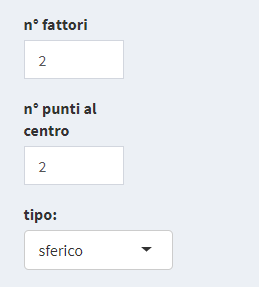
\includegraphics[width=1\linewidth]{Immagini/CCD/02_disegno_esempio} 

}

\caption{Scelta numero fattori, punti al centro e tipo di CCD nell'applicativo}\label{fig:ccd2}
\end{figure}

Ognuna delle 3 risposte sarà analizzata con il modello quadratico Figura \ref{fig:ccd3}. Dalla lettura della matrice di dispersione si nota la non ortogonalità del modello (i termini quadratici sono correlati tra di loro, v. riquadro colorato in giallo nella Figura).

\begin{figure}[ht]

{\centering 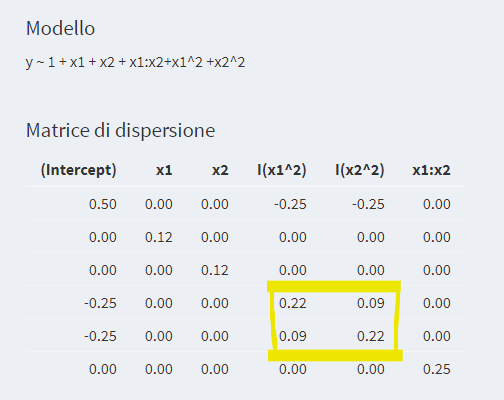
\includegraphics[width=1\linewidth]{Immagini/CCD/03_matrdisp} 

}

\caption{Modello e matrice di dispersione del CCD}\label{fig:ccd3}
\end{figure}

Le linee di livello del Leverage Figura \ref{fig:ccd4} mettono in evidenza invece la ruotabilità del piano sperimentale scelto.

\begin{figure}[ht]

{\centering 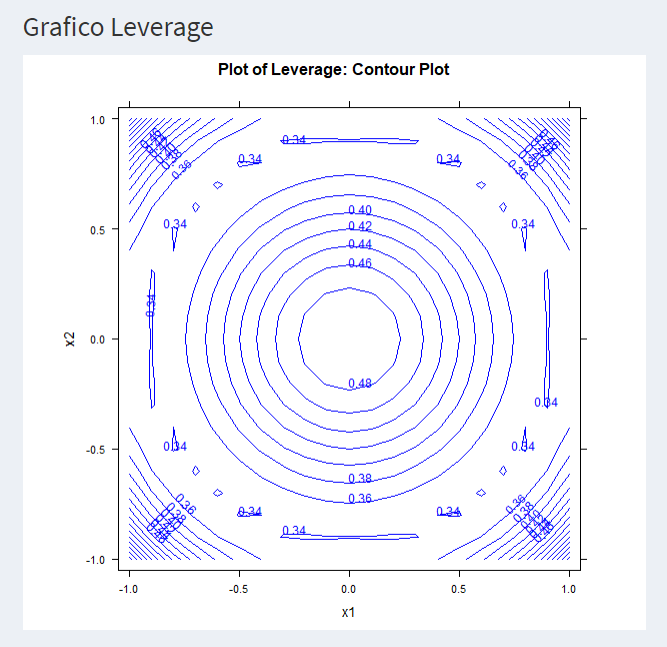
\includegraphics[width=1\linewidth]{Immagini/CCD/04_livello} 

}

\caption{Grafico delle linee di livello del Leverage}\label{fig:ccd4}
\end{figure}

Procediamo come di consueto inserendo le Risposte nell'apposito riquadro. Una volta convalidato il modello con tre misure indipendenti Tabella \ref{tab:matrconv}
\newpage

\begin{table}

\caption{\label{tab:matrconv}Misure indipendenti per convalidare il modello}
\centering
\begin{tabular}[t]{lrrrrrrr}
\toprule
  & Time & Temp & X1 & X2 & Y1 & Y2 & Y3\\
\midrule
11 & 85 & 175 & 0 & 0 & 80.0 & 68 & 3410\\
12 & 85 & 175 & 0 & 0 & 79.7 & 70 & 3290\\
13 & 85 & 175 & 0 & 0 & 79.8 & 71 & 3500\\
\bottomrule
\end{tabular}
\end{table}

possiamo utilizzare il grafico delle linee di livello Figura \ref{fig:ccd5} per confrontare le risposte tra di loro.

\begin{figure}[ht]
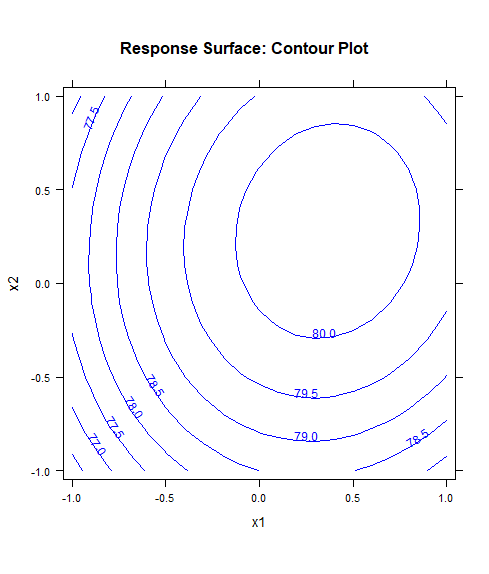
\includegraphics[width=0.5\linewidth]{Immagini/CCD/05_liv1} 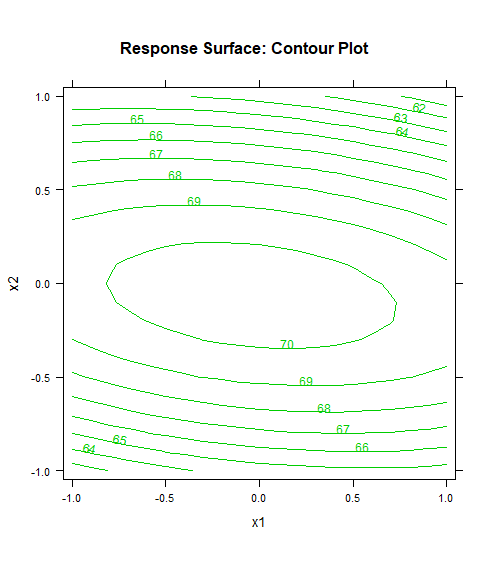
\includegraphics[width=0.5\linewidth]{Immagini/CCD/06_liv2} 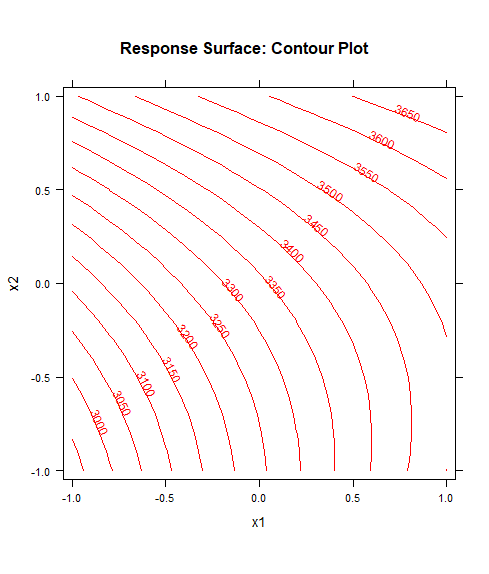
\includegraphics[width=0.5\linewidth]{Immagini/CCD/07_liv3} \caption{Grafico delle linee di livello delle risposte $Y_1,Y_2$ e $Y_3$}\label{fig:ccd5}
\end{figure}

Nell'applicativo si noti che è possibile scegliere il colore delle linee di livello. Questa risorsa è utile quando, come in questo caso, bisogna confrontare più grafici tra loro Figura \ref{fig:ccd8}.

\begin{figure}[ht]
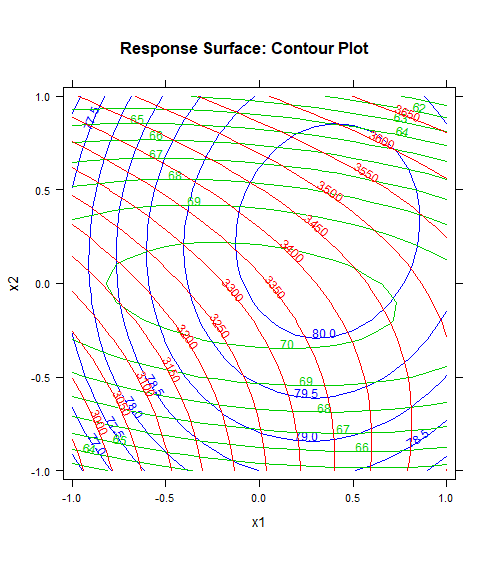
\includegraphics[width=0.5\linewidth]{Immagini/CCD/08_livelli} 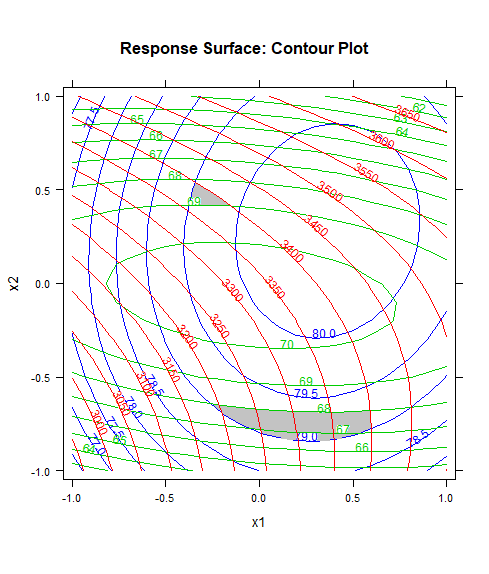
\includegraphics[width=0.5\linewidth]{Immagini/CCD/09_livelli} \caption{Grafici delle linee di livello delle risposte $Y_1,Y_2$ e $Y_3$ sovrapposti e regione di ottimo}\label{fig:ccd8}
\end{figure}

Analizzando i vincoli e le linee di livello della resa \(Y_1\) si vede che le zona in cui cercare soluzione del problema sono quelle colorate in grigio (v. Figura \ref{fig:ccd8}).

\hypertarget{disegni-d-ottimali}{%
\chapter{Disegni D-ottimali}\label{disegni-d-ottimali}}

Nelle sezioni precedenti sono stati illustrati disegni in cui la geometria del dominio sperimentale (iperpiano, ipercubo, ipersfera) e il modello erano prefissati (modello primo ordine, lineare senza interazioni, di secondo ordine lineare con interazioni di coppie di termini, di secondo ordine con interazioni a coppie e con termini quadratici). Questi piani sperimentali e i corrispondenti modelli sono ``ottimali'' e garantiscono la massima efficienza nella sperimentazione, vale a dire l'ottenimento della informazione di migliore qualità con il numero minimo di esperimenti possibile.
Tuttavia esistono molte situazioni in cui i disegni fino ad ora visti possono non essere la scelta ``migliore''. I casi più comuni in cui è difficile impiegare proficuamente i disegni canonici visti finora sono:

\begin{itemize}
\tightlist
\item
  la regione sperimentale non è una figura geometrica regolare: si devono rispettare condizioni di lavoro prestabilite - vincoli;
\item
  il modello è non canonico: ad esempio contiene un termine quadratico in una variabile ma non nelle altre, oppure contiene fattori quantitativi e almeno un fattore qualitativo a più di due livelli (es. la regolazione di uno strumento è possibile solo su tre livelli non numerici indicati con ``basso'', ``medio'' e ``alto'')
\item
  il numero di esperimenti fattibili non è sufficiente per completare i disegni fino ad ora visti per qualsiasi ragione (es. indisponibilità di risorse, di tempo) .
\end{itemize}

In tutti questi casi, non è mai una buona decisione quella di adattare artificiosamente la sperimentazione ad un disegno sperimentale e ad un modello canonico. Piuttosto conviene pensare quali possono essere il modello e il piano sperimentale migliori per studiare il problema in osservazione.
La soluzione a questi problemi che proponiamo in questo corso e nell'applicativo è fornita dai cosiddetti \emph{disegni D-ottimali}.
La costruzione dei disegni D-ottimali è condotta come segue.
Fissata la regione sperimentale da stusiare, scegliamo in tale regione un insieme di \(m\) punti (leggi: esperimenti) candidati ad essere usati per costruire un disegno ad-hoc per il nostro problema. In generale si considera una griglia di punti che copre l'intera regione da studiare con un dettaglio (leggi: ampiezza degli intervalli che costituiscono la griglia dei punti sperimentali) che dipende dagli obiettivi dello studio.\\
Si scelgono quindi un modello contenente \(p\) parametri e il numero \(n\)
\begin{equation*}
p \leq n \leq m
\end{equation*}
di esperimenti che vogliamo eseguire. Fatte queste scelte la matematica ci consente di sapere che esistono
\begin{equation*}
\frac{m!}{(m-n)!n!}
\end{equation*}
matrici sperimentali possibili. Per scegliere il ``disegno migliore'' tra queste \(\frac{m!}{(m-n)!n!}\) matrici esistono vari criteri. In questa dispensa ci occuperemo del criterio cosiddetto di \emph{\(D\)-ottimalità} e di quei disegni, definiti per questo \emph{D-ottimali}, che soddisfano tale criterio di scelta. Tali disegni sono quelli che massimizzano il determinante della matrice di informazione.
\begin{equation*}
\rm{det}(X^tX).
\end{equation*}
Maggiore è il determinante della matrice di informazione ``migliore'' è l'ortogonalità del modello. Si può dimostrare che la radice del determinate della matrice di informazione è inversamente proporzionale al volume dell'iperelissoide di confidenza dei parametri del modello. Massimizzare il determinante della matrice di informazione corrisponde a rendere di migliore qualità l'informazione sui parametri del modello (i.e.~rendere minima la loro varianza) e ottenere quindi la predizione più precisa della variabile risposta.\newline
I disegni canonici fino ad ora considerati sono tutti \(D\)-ottimali.

Per poter confrontare disegni che differiscono per il numero di esperimenti progettati \(n\) (ad esempio, un disegno non canonico in cui è possibile avere più repliche di esperimenti nel dominio sperimentale) introduciamo il seguente indicatore \(0 \leq D \leq 1\)
\begin{equation}
    D=\frac{\rm{det}(X^tX)^{1/p}}{n}
    \label{eq:DOpt}
\end{equation}
che misura la ``qualità'' del disegno considerato. Si noti che in generale per piani sperimentali multivariati non è vero che all'aumentare di \(n\) abbiamo una migliore ``qualità'' del disegno (cf.~Figura \ref{fig:fig3}). Questo criterio vale solo per studi limitati alla misura dell'effetto di un solo fattore. L'indicatore \(D\) trova il miglior compromesso tra maggiore informazione (determinante della matrice di informazione) e lo ``sforzo'' sperimentale (il numero \(n\) di esperimenti).\newline
Indicando rispettivamente con \(D_1\) e \(D_2\) l'indicatore (\ref{eq:DOpt}) per un piano sperimentale costruito con un disegno avente numero di esperimenti differenti \(n_1\) e \(n_2\), l'efficacia relativa tra i due progetti si ottiene del rapporto \(D_1/D_2\).

\hypertarget{algoritmo-di-federov}{%
\section{Algoritmo di Federov}\label{algoritmo-di-federov}}

Descriviamo brevemente l'algoritmo di Federov, su cui è basato l'applicativo, per determinare disegni \(D\)-ottimali.

Sia \(X_n\) la matrice del modello di un disegno di \(n\) esperimenti. Indichiamo con \(X_{n+1}\) la matrice del modello del disegno di \(n+1\) punti sperimentali ottenuta aggiungendo a \(X_n\) un nuovo punto \(x^j\). La corrispondente matrice di informazione è data
\begin{equation*}
    X^t_{n+1}X_{n+1}=X^t_nX_n+(x^j*x^{jt})
\end{equation*}
il cui determinante soddisfa
\begin{equation*}
    \rm{det}(X^t_{n+1}X_{n+1})=\rm{det}(X^t_nX_n)(1+h(x^j)),
\end{equation*}
dove \(h(x^j)=x^j(X^t_nX_n){-1}x^{jt}\) è il valore Leverage di \(x^j\). \newline
In maniera analoga, indicando con \(X_{n-1}\) la matrice del modello del disegno di \(n-1\) punti sperimentali ottenuto rimuovendo da \(X_n\) un punto \(x_i\), la corrispondente matrice di informazione è data
\begin{equation*}
    X^t_{n-1}X_{n-1}=X^t_nX_n+(x_i*x^t_i)
\end{equation*}
il cui determinante soddisfa
\begin{equation*}
    \rm{det}(X^t_{n-1}X_{n-1})=\rm{det}(X^t_nX_n)(1-h(x_i)),
\end{equation*}
dove \(h(x_i)=x_i(X^t_nX_n)^{-1}x^t_i\) è il valore Leverage di \(x_i\).

Nell'algoritmo di Federov lo scambio tra un punto sperimentale \(x^j\) appartenete all'insieme dei punti candidati e un punto \(x_i\) appartenente al disegno iniziale avviene simultaneamente ottenendo un nuovo disegno la cui matrice del modello \(\tilde{X}_n\) ha la corrispondente matrice di informazione legata alla precedente da
\begin{equation*}
    \tilde{X_n}^t\tilde{X_n}=X^t_{n}X_{n}-(x_i*x_i^t)+(x^j*x^{jt})
\end{equation*}
il cui determinante soddisfa
\begin{equation*}
    \rm{det}(\tilde{X_n}^t\tilde{X_n})=\rm{det}(X^t_{n}X_{n})(1+\Delta(x_i,x^j)),
\end{equation*}
dove
\begin{equation*}
    \Delta(x_i,x^j)=h(x^j)-(h(x_i)h(x^j)-h(x_i,x^j)^2)-h(x_i)
\end{equation*}
con \(h(x_i,x^j)=x_i^t(X^tX)x^j=x^j(X^tX)x_i.\)

L'algoritmo di Federov sceglie casualmente \(n\) punti nell'insieme dei punti candidati, ne calcola la matrice del modello \(X\) e quindi determina il valore \(\Delta(x_i,x^j)\) per ogni coppia di \((x_i,x^j)\) con \(x_i\) appartenente al disegno scelto casualmente e \(x^j\) appartenente all'insieme dei punti candidati (esclusi gli \(n\) punti scelti). La procedura di calcolo individua una coppia di esperimenti \((x_i,x^j)\) per cui \(\Delta(x_i,x^j)\) sia positivo e massimo e quindi scambia \(x_i\) con \(x^j\). A partire dal nuovo insieme di \(n\) punti ripete il procedimento finché non trova una coppia di punti \((x_i,x^j)\) con \(\Delta(x_i,x^j)>0\). Nei vari software di calcolo il procedimento si ferma quando \(\Delta(x_i,x^j)\) raggiunge un valore sufficientemente piccolo.

\hypertarget{esempio-proprietuxe0-di-un-adesivo}{%
\section{Esempio: proprietà di un adesivo}\label{esempio-proprietuxe0-di-un-adesivo}}

Uno sperimentatore sta indagando sulle proprietà di un
particolare adesivo termoplastico. L'adesivo è applicato su due parti di pezzi che vengono incollati tra loro e quindi trattati a temperature diverse. I
due fattori di interesse sono

\begin{itemize}
\tightlist
\item
  \(X_1\) la quantità di adesivo applicato
\item
  \(X_2\) la temperatura.
\end{itemize}

La variabile risposta \(Y\) è la forza con cui le due parti di ogni pezzo risultano incollate, misurata dalla cosiddetta ``forza di strappo''. Questa risposta è descritta con un modello del secondo ordine
\[
Y=b_0+b_1X_1+b_2X_2+b_{11}X_1^2+b_{22}X_2^2+b_{12}X_1X_2
\]

Considerando il dominio standardizzato, le variabili \(X_1\) e \(X_2\) variano tra \(-1\) e \(1\). Lo sperimentatore sa che se viene applicato troppo poco adesivo e la temperatura è troppo bassa, le parti non si incollano. Si impone quindi il vincolo
\[
X_1+X_2\geq-1.5
\]
Inoltre, se la temperatura del trattamento termico è troppo alta e si applica troppo adesivo, le parti incollate si rovinano per effetto di stress da calore, oppure non si incollano bene. Si impone quindi anche un secondo vincolo
\[
X_1+X_2\leq 1
\]

Scegliamo nella regione sperimentale un insieme di punti candidati ad essere usati per un disegno. Stabiliamo ad esempio di usare una griglia di passo 0.1. Per generare la matrice dei punti candidati nell'applicativo, si seleziona il menù D-ottimale alla pagina Matrice punti candidati, e si scelgono le opzioni del caso in esame come in Figura \ref{fig:fig1}

\begin{figure}[ht]

{\centering 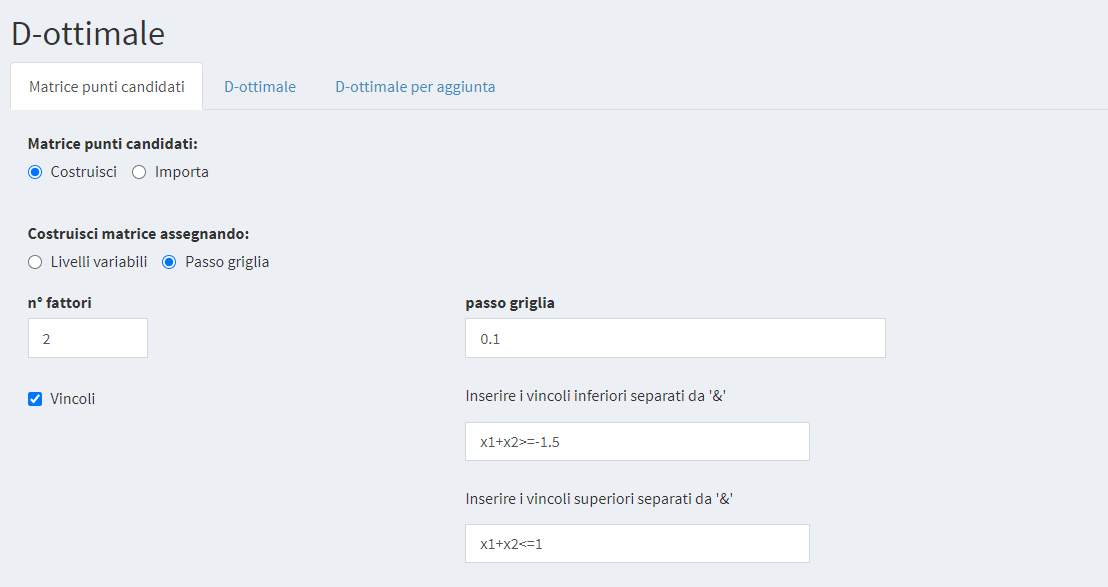
\includegraphics[width=1\linewidth]{Immagini/D_opt/01_es1_pticandidati} 

}

\caption{Costruzione della matrice dei punti candidati}\label{fig:fig1}
\end{figure}

Si noti come sono stati indicati i vincoli. Se si vuole, è possibile scaricare la matrice dei punti candidati generata con il tasto Download. In Figura \ref{fig:fig2} è illustrata graficamente la forma del dominio sperimentale dei punti del caso in discussione, realizzata con Excel.

\begin{figure}[ht]

{\centering 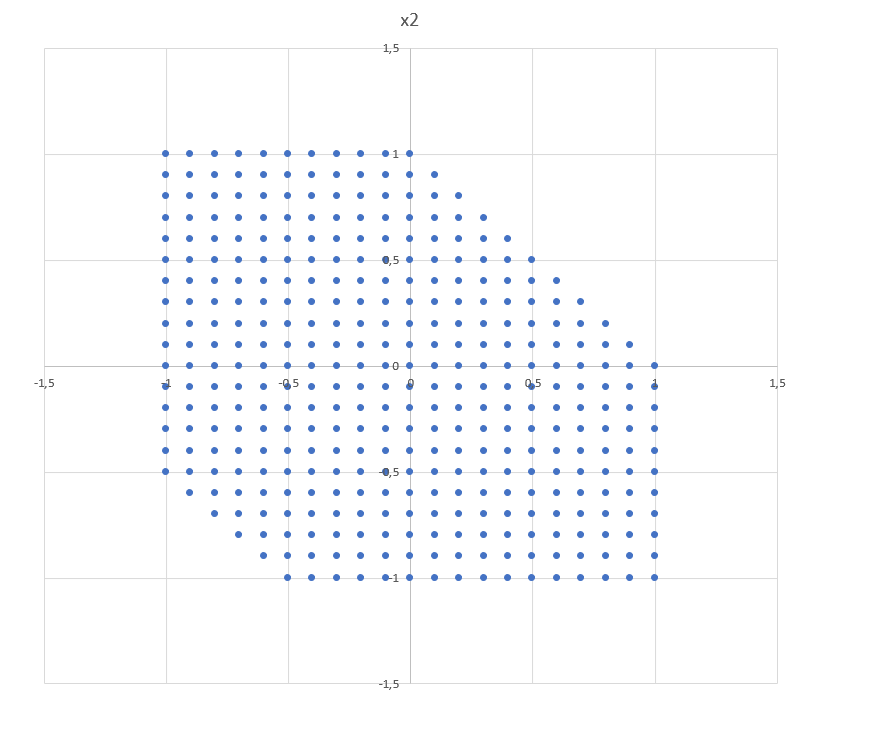
\includegraphics[width=1\linewidth]{Immagini/D_opt/02_es1_pticandidati} 

}

\caption{Insieme dei punti candidati}\label{fig:fig2}
\end{figure}

Nella pagina D-ottimale Figura \ref{fig:fig3} una volta fissato il modello e il numero massimo di esperimenti, cliccando sul bottone Calcola viene determinato il piano sperimentale D-ottimale per ogni numero di esperimenti tra il minimo e il massimo fissati nell'applicativo. Sono anche dati i valori del parametro \(D\) definito in \eqref{eq:DOpt} e il valore di VIF massimo. Possiamo vedere l'andamento di questi valori in funzione del numero di esperimenti in Figura \ref{fig:fig3}

\begin{figure}[ht]
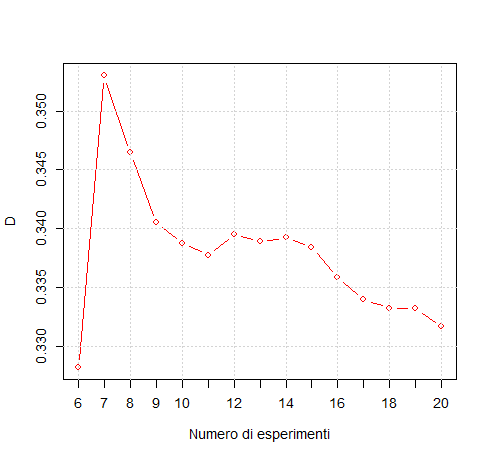
\includegraphics[width=0.5\linewidth]{Immagini/D_opt/04_es1_pticandidati} \includegraphics[width=0.5\linewidth]{Immagini/D_opt/05_es1_pticandidati} \caption{Andamento del parametro $D$ e del VIF massimo in funzione del numero di esperimenti}\label{fig:fig3}
\end{figure}

Come si può vedere in Figura \ref{fig:fig3} il ``migliore'' valore di \(D\) è dato dal piano con 7 esperimenti Figura \ref{fig:fig6} e Figura \ref{fig:fig7}

\begin{figure}[ht]

{\centering \includegraphics[width=1\linewidth]{Immagini/D_opt/06_es1_pticandidati} 

}

\caption{Disegno D-ottimale}\label{fig:fig6}
\end{figure}
\begin{figure}[ht]

{\centering \includegraphics[width=1\linewidth]{Immagini/D_opt/07_es1_pticandidati} 

}

\caption{Disegno D-ottimale}\label{fig:fig7}
\end{figure}

\hypertarget{esempio-riparazione-di-una-matrice}{%
\section{Esempio: riparazione di una matrice}\label{esempio-riparazione-di-una-matrice}}

I disegni D-ottimali possono essere usati per ``riparare'' matrici i cui gli esperimenti sono stati eseguiti senza seguire un piano sperimentale predeterminato
definendo l'insieme degli esperimenti possibili (insieme dei punti candidati) e tenendo ``bloccati'' gli esperimenti già eseguiti.
Vediamo un esempio.

Per ottimizzare un metodo cromatografico \citep{r.leardi2018} è stato utilizzato un CCD a facce centrate con 4 variabili e 5 repliche al centro per un totale di 29 esperimenti.
Dopo che ci si è resi conto che il livello superiore di \(X_3\) era troppo alto (tutti i 9 esperimenti eseguiti con \(X_3\) = 1 sono falliti). Non era più possibile avere sufficiente informazione dai 16 esperimenti ``buoni'' di cui 1 replicato 5 volte (punti al centro).\\
Fu deciso di tenere il precedente livello inferiore di \(X_3\) ma di utilizzare il livello centrale del primo piano di esperimenti come nuovo livello superiore e di fissare un nuovo livello centrale nel punto medio dei due nuovi livelli Tabella \ref{tab:Esbuoni}

\begin{table}

\caption{\label{tab:Esbuoni}I 16 esperimenti "buoni" di cui 1 replicato 5 volte}
\centering
\begin{tabular}[t]{rrrrr}
\toprule
Exp. & x1 & x2 & x3 & x4\\
\midrule
1 & -1 & -1 & -1 & -1\\
2 & 1 & -1 & -1 & -1\\
3 & -1 & 1 & -1 & -1\\
4 & 1 & 1 & -1 & -1\\
5 & -1 & -1 & -1 & 1\\
\addlinespace
6 & 1 & -1 & -1 & 1\\
7 & -1 & 1 & -1 & 1\\
8 & 1 & 1 & -1 & 1\\
9 & -1 & 0 & 1 & 0\\
10 & 1 & 0 & 1 & 0\\
\addlinespace
11 & 0 & -1 & 1 & 0\\
12 & 0 & 1 & 1 & 0\\
13 & 0 & 0 & -1 & 0\\
14 & 0 & 0 & 1 & -1\\
15 & 0 & 0 & 1 & 1\\
\addlinespace
16 & 0 & 0 & 1 & 0\\
17 & 0 & 0 & 1 & 0\\
18 & 0 & 0 & 1 & 0\\
19 & 0 & 0 & 1 & 0\\
20 & 0 & 0 & 1 & 0\\
\bottomrule
\end{tabular}
\end{table}

Gli esperimenti possibili tra cui scegliere i punti da introdurre nel piano sperimentale da ``aggiustare'' sono tutti i \(3^4\) esperimenti possibili con \(4\) fattori studiati a \(3\) livelli (-1,0,1), e da questi vanno tolti i 16 esperimenti già eseguiti. Per costruire l'insieme di tutte le combinazioni dei 4 fattori con l'applicativo nella pagina Matrice punti candidati del menù D-ottimale si indicano i livelli per ogni variabile come in Figura \ref{fig:fig10}

\begin{figure}[ht]

{\centering \includegraphics[width=1\linewidth]{Immagini/D_opt/10_es2} 

}

\caption{Costruzione dei punti candidati indicando i livelli}\label{fig:fig10}
\end{figure}

Una volta ``ripulito'' il dataset creato dai 16 esperimenti già eseguiti lo si importa nella pagina Matrice punti candidati. Quindi si importano nella pagina D-ottimale per aggiunta i 16 esperimenti già eseguiti e, una volta fissati il numero minimo e massimo di esperimenti totali (20 già eseguiti: 16 più 5 repliche, quindi almeno 21), cliccando sul bottone Calcola si ottiene il piano sperimentale D-ottimale. L'operazione è condotta seguendo la stessa logica descritta per la pagina D-ottimale, Figura \ref{fig:fig8}

\begin{figure}[ht]
\includegraphics[width=0.5\linewidth]{Immagini/D_opt/08_es2} \includegraphics[width=0.5\linewidth]{Immagini/D_opt/09_es2} \caption{Andamento del parametro $D$ e VIF max in funzionedel Numero di esperimenti}\label{fig:fig8}
\end{figure}

Nell'esempio in discussione, il compromesso scelto fu quello di aggiungere 11 esperimenti ai 20 già eseguiti. La soluzione detta fu adottata considerando il basso costo di ogni esperimento. Come spesso accade però nelle analisi di esperimenti condotte \emph{a posteriori}, se si riconsidera il problema più attentamente, si può osservare che aggiungendo un solo esperimento si ottiene una soluzione più che accettabile.

Nota: l'algoritmo di Federov è conosciuto da oltre 40 anni ed è uno degli algoritmi più studiati per calcoli di disegni D-ottimali \citep{v.v.federov1972}. Negli anni, molti studiosi hanno sviluppato varianti di questo algoritmo presentate come più veloci ed efficienti, per cui usando sofware commerciali (es. Minitab, Design Expert, JMP) può capitare di dovere scegliere tra più opzioni di metodi per il calcolo di piani sperimentali ottimali. In questi software, l'algoritmo di Federov originale è chiamato ``algoritmo di scambio'', e le versioni modificate fanno ricorso a sistemi meno laboriosi dal punto di vista del calcolo per la scelta dei punti su cui eseguire lo scambio descritto in questa sezione.

\hypertarget{miscele}{%
\chapter{Miscele}\label{miscele}}

In un esperimento con miscele i \(k\) fattori \(X_1, \dots, X_k\) sono le differenti proporzioni dei costituenti della miscela, e queste devono soddisfare il seguente vincolo
\begin{equation}
    X_1+\cdots+X_k=1.
    \label{eq:VinMisc}
 \end{equation}
Il fatto che la somma delle proporzioni dei differenti fattori debba essere uguale a \(1\) complica il disegno sperimentale e l'analisi dei risultati. Il dominio sperimentale può avere forma geometrica regolare (triangolare \(\mathbb{R}^2\), tetraedrica in \(\mathbb{R}^3\), ipertetraedrica in \(\mathbb{R}^k\)), oppure poligonale o iperpoliedrica irregolare se le proporzioni stesse sono condizionate da vincoli particolari.
Nel caso caso di \(3\) fattori si può rappresentare bidimensionalmente il dominio sperimentale mediante un diagramma ternario (vedi Figura \ref{fig:MiscDiaTern})

\begin{figure}
\centering
\includegraphics{dispense_doe_files/figure-latex/MiscDiaTern-1.pdf}
\caption{\label{fig:MiscDiaTern}Diagramma ternario (\(p=(20,40,40)\))}
\end{figure}

in cui è rappresentato il punto di coordinate \(p=(0.2,0.4,0.4)\). Si noti che in Figura \ref{fig:MiscDiaTern} le coordinate sono date in percentuale e non in proporzione, ossia \(p=(20,40,40)\).

In questo dominio dovremo ricavare, mediante opportuno disegno sperimentale, l'ottimo della risposta e conoscere come varia la risposta nel dominio sperimentale.
Oltre a questo vincolo primario possono esserci ulteriori vincoli e ciò complica ancora di più la situazione.

Consideriamo ora i modelli per disegni di miscele. Non tutti i modelli utilizzati fino ad ora potranno essere definiti in quanto per alcuni di essi la relativa matrice d'informazione non è invertibile per l'esistenza del vincolo \eqref{eq:VinMisc} che rende non indipendenti tra loro i fattori del disegno.
Ad esempio l'usuale modello del primo ordine
\begin{equation*}
    Y=\beta_0+\sum_{i=1}^k\beta_iX_i+\epsilon
\end{equation*}
ha matrice d'informazione singolare essendo per il vincolo (\ref{eq:VinMisc}) la colonna \emph{Int.} somma delle colonne \(X_1,\dots,X_k\). Si può pensare di eliminare uno dei fattori ponendo che ad es. \(X_j=1-\sum_{i\neq j}X_i\) ma il migliore approccio è stato finora quello suggerito da Sheffé. La soluzione proposta da Sheffé fu di moltiplicare \(\beta_0\) per \(1=\sum_iX_i\) per ottenere
\begin{equation*}
    Y=\sum_{i=1}^k(\beta_0+\beta_i)X_i+\epsilon.
\end{equation*}
Analogamente l'usuale modello quadratico
\begin{equation*}
    Y=\sum_{i=1}^k\beta_iX_i+\sum_{i=1}^k\sum_{j>i}\beta_{ij}X_iX_j+\sum_{i=1}^k\beta_{ii}X_i^2+
    \epsilon
\end{equation*}
ha matrice d'informazione singolare essendo per il vincolo \eqref{eq:VinMisc}
\begin{equation*}
    X_i^2=X_iX_i=X_i(1-\sum_{j\neq i}X_j)=X_i-\sum_{j\neq i}X_iX_j.
\end{equation*}
In questo caso si può eliminare
\(X_i^2=X_i-\sum_{j\neq i}X_iX_j\) ottenendo
\begin{equation*}
    Y=\sum_{i=1}^k(\beta_i+\beta_{ii})X_i++\sum_{i=1}^k\sum_{j>i}(\beta_{ij}-\beta_{ii}-\beta_{jj})X_iX_j
    +\epsilon.
\end{equation*}
Ragionamenti analoghi possono essere fatti per i modelli di ordine superiore.
Riassumendo, riordinando i parametri, abbiamo i quattro tipi di modelli seguenti

\begin{itemize}
\tightlist
\item
  \textbf{Lineare}
  \begin{equation*}
    Y=\sum_{i=1}^k\beta_iX_i+\epsilon
  \end{equation*}
\item
  \textbf{Quadratico}
  \begin{equation*}
    Y=\sum_{i=1}^k\beta_iX_i+\sum_{i=1}^k\sum_{j>i}\beta_{ij}X_iX_j+\epsilon
  \end{equation*}
\item
  \textbf{Cubico speciale}
  \begin{equation*}
    Y=\sum_{i=1}^k\beta_iX_i+\sum_{i=1}^k\sum_{j>i}\beta_{ij}X_iX_j+
    +\sum_{i=1}^k\sum_{j>i}\sum_{k>j}\beta_{ijk}X_iX_jX_k+\epsilon
  \end{equation*}
\item
  \textbf{Cubico completo}
  \begin{equation*}
    Y=\sum_{i=1}^k\beta_iX_i+\sum_{i=1}^k\sum_{j>i}\beta_{ij}X_iX_j+
    +\sum_{i=1}^k\sum_{j>i}\delta_{ij}X_iX_j(X_i-X_j)+
    +\sum_{i=1}^k\sum_{j>i}\sum_{k>j}\beta_{ijk}X_iX_jX_k+\epsilon.
  \end{equation*}
\end{itemize}

Come accennato all'inizio di questa sezione i fattori dei disegni di miscele non sono variabili indipendenti tra loro come invece accadeva nei disegni canonici finora studiati. I fattori dei disegni di miscele sono legati dal vincolo \eqref{eq:VinMisc}, e pertanto bisogna fare molta attenzione al significato dei coefficenti del modello. I termini lineari \(\beta_i\), infatti, non rappresentano l'effetto dei fattori \(X_i\) sulla risposta, se fissiamo gli altri fattori pari a 0 come si poteva fare nei disegni canonici visti finora. Nei disegni di miscele, non c'è intercetta, perché la miscela ``nulla'' non ha senso fisico. Inoltre è impossibile stimare l'effetto di un solo fattore indipendentemente dagli altri per l'esistenza del vincolo \eqref{eq:VinMisc}: se osserviamo un solo fattore \(X_i\), le altre k-1 variabili non possono essere contemporaneamente tutte nulle; questa situazione sperimentalmente sarebbe quella data dalla miscela pura \(X_i=1\), Figura \ref{fig:mixfig2}.

\begin{figure}[ht]

{\centering \includegraphics[width=1\linewidth]{Immagini/Mixt/02_coeff_lin} 

}

\caption{Intepretazione dei termini lineari}\label{fig:mixfig2}
\end{figure}

Anche nel caso in cui \(\beta_i=0\), ciò non significa che l'effetto del fattore i-esimo sulla risposta variando \(X_i\) da 0 a 1, sia nullo, nemmeno mantenendo ad esempio costante il rapporto tra le altre variabili \(\frac{X_1}{X_2}=1\). Il vincolo per cui la somma delle proporzioni dei fattori è uguale a 1, impone che non possiamo mantenere nulle le tre variabili e quindi dobbiamo ``scegliere una direzione nel dominio sperimentale lungo cui fare variare il fattore'' in esame e modificare simultaneamente le proporzioni dei rimanenti k-1 in modo tale che sia rispettato il vincolo di costruzione della miscela. Ad esempio in Figura \ref{fig:mixfig1} sono indicate le risposte per le miscele pure \(X_i=1\) e per la miscela \(X_2=X_3=05\) dato il modello \(Y=5X_2+4X_3\)

\begin{figure}[ht]

{\centering \includegraphics[width=1\linewidth]{Immagini/Mixt/01_coeff_effetto} 

}

\caption{"Effetto" per un termine il cui coeffciente è nullo}\label{fig:mixfig1}
\end{figure}

Come si può osservare, l'effetto dovuto alla variazione di \(X_1\) da 0 a 1 muovendosi lungo la linea tratteggiata (linea lungo la quale \(\frac{X_1}{X_2}=1\)) è -4.5 pur essendo \(\beta_1=0\).

I termini misti \(\beta_{ij}\) non vanno interpretati come termini di interazione ma, a differenza delle variabili indipendenti, come termini di miscelazione non lineare: ciò equivale a dire che se \(\beta_{ij}>0\) la miscela tra \(X_i\) e \(X_j\) ha effetto positivo sulla risposta \(Y\). Per un'interpretazione grafica si veda Figura \ref{fig:mixfig3}

\begin{figure}[ht]

{\centering \includegraphics[width=1\linewidth]{Immagini/Mixt/03_coeff_quadr} 

}

\caption{Interpretazione dei termini quadratici\label{fig3}}\label{fig:mixfig3}
\end{figure}

Il coefficiente \(\beta_{123}\) rappresenta invece la miscela ternaria dei 3 componenti all'interno del simplesso (1/27 del suo valore corrisponde all'altezza/profondità della superficie di riposta nel centro del simplesso).

Nell'applicativo nel menù Miscele/Simplex Design per ognuno dei modelli lineare, quadratico e cubico è proposto un disegno Figura \ref{fig:mixfig4}

\begin{figure}[ht]
\includegraphics[width=0.5\linewidth]{Immagini/Mixt/04_dis_lin} \includegraphics[width=0.5\linewidth]{Immagini/Mixt/05_dis_quad} \includegraphics[width=0.5\linewidth]{Immagini/Mixt/06_dis_cub} \includegraphics[width=0.5\linewidth]{Immagini/Mixt/07_dis_cub} \caption{Simplex Design per modello lineare, quadratico e cubico senza e  con punti assiali }\label{fig:mixfig4}
\end{figure}

E' possibile anche aggiungere ulteriori punti (punti assiali) all'interno del simplesso dove la precisione di un modello può essere verificata.

\hypertarget{esempio-ace}{%
\section{Esempio: ACE}\label{esempio-ace}}

Disponendo in casa di una elettrodomestico per preparare centrifugati di frutta e verdura si è studiata la composizione ``più buona'' delle bevande ACE. Al netto dell'acqua, che in generale è circa il 70\% della bevanda, si è voluta studiare la ``migliore'' miscela ottenuta con

\begin{itemize}
\tightlist
\item
  \(x_1\) arancia
\item
  \(x_2\) carota
\item
  \(x_3\) limone
\end{itemize}

Nota bene: la percentuale 100\% delle 3 sostanze rappresenta il 70\% della bevanda.

Si è scelto di utilizzare il modello cubico. La bevanda ottenuta è stata quindi valutata da 4 assaggiatori (ogni volta in ordine casuale e mascherandone il colore), e questi hanno espresso un voto sulla ``bontà''. I voti sono stati quindi scalati da 0 a 100 (i voti erano espressi in decimi) per evitare l'evenienza di avere differenti intervalli di variazione del voto. I risulati ottenuti sono riportati in Tabella \ref{tab:ace}

\begin{table}

\caption{\label{tab:ace}Disegno sperimentale e risultati per la bevanda ACE}
\centering
\begin{tabular}[t]{r|r|r|r|r|r|r}
\hline
x1 & x2 & x3 & R & P & M & D\\
\hline
1.0000 & 0.0000 & 0.0000 & 75 & 83.3 & 50 & 87.5\\
\hline
0.0000 & 1.0000 & 0.0000 & 50 & 66.7 & 25 & 100.0\\
\hline
0.0000 & 0.0000 & 1.0000 & 0 & 50.0 & 0 & 12.5\\
\hline
0.5000 & 0.5000 & 0.0000 & 100 & 100.0 & 75 & 62.5\\
\hline
0.5000 & 0.0000 & 0.5000 & 25 & 33.3 & 50 & 0.0\\
\hline
0.0000 & 0.5000 & 0.5000 & 50 & 100.0 & 25 & 25.0\\
\hline
0.3333 & 0.3333 & 0.3333 & 25 & 0.0 & 100 & 75.0\\
\hline
\end{tabular}
\end{table}

Riportando i voti dati da ogni assaggiatore nell'applicativo si ottengono le seguenti superfici di risposta Figura \ref{fig:mixfig8}

\begin{figure}[ht]
\includegraphics[width=0.5\linewidth]{Immagini/Mixt/08_aceR} \includegraphics[width=0.5\linewidth]{Immagini/Mixt/09_aceP} \includegraphics[width=0.5\linewidth]{Immagini/Mixt/10_aceM} \includegraphics[width=0.5\linewidth]{Immagini/Mixt/11_aceD} \caption{Superfici di risposta del voto espresso dai 4 assaggiatori}\label{fig:mixfig8}
\end{figure}

\newpage

\hypertarget{diegni-di-miscele-d-ottimali}{%
\section{Diegni di miscele D-ottimali}\label{diegni-di-miscele-d-ottimali}}

Frequentemente oltre al vincolo \eqref{eq:VinMisc}, nello studio di miscele vengono imposti altri vincoli. Ciò implica che si determinano domini sperimentali poligonali irregolari che, in generale, non permettono l'uso di nessuno dei quattro modelli canonici elencati più sopra. In questi casi si può procedere solo costruendo disegni D-ottimali che visto per disegni in cui le variabili sono indipendenti.

Consideriamo, per capire come si procede, il seguente esempio

\hypertarget{esempio-polveron}{%
\subsection{Esempio: Polveron}\label{esempio-polveron}}

Si cerca di valutare l'apprezzamento dei consumatori di un Polveron, dolce tipico delle Filippine, composto da una miscela di \(x_1\) zucchero, \(x_2\) arachidi e \(x_3\) burro.\\
Questi ingredienti devono soddisfare i seguenti vincoli
\begin{eqnarray*}
  0.00& \leq x1 \leq & 0.80\\
  0.10&\leq x2 \leq & 0.95 \\
  0.05&\leq x3 \leq & 0.50
\end{eqnarray*}

Cominciamo con il costruire il dominio sperimentale e l'insieme dei punti candidati mediante l'applicativo. Nel menù Miscele/D-ottimale alla pagina Matrice punti candidati si definisca il passo della griglia scelto e si indichino i vincoli come in Figura \ref{fig:mixfig17}

\begin{figure}[ht]

{\centering \includegraphics[width=1\linewidth]{Immagini/Mixt/17_cp} 

}

\caption{Costruzione dell'insieme dei punti candidati}\label{fig:mixfig17}
\end{figure}

Si calcola la matrice dei punti candidati e ne viene data una rappresentazione grafica Figura \ref{fig:mixfig18}

\begin{figure}[ht]

{\centering \includegraphics[width=1\linewidth]{Immagini/Mixt/18_cp} 

}

\caption{Matrice dei punti candidati e rappresentazione grafica}\label{fig:mixfig18}
\end{figure}

La matrice dei punti candidati è esportabile cliccando sul bottone \emph{Download}.

Passando quindi alla pagina D-ottimale si indicano i termini del modello che si vuole studiare e il numero minimo e massimo di esperimenti Figura \ref{fig:mixfig19}. Quindi cliccando sul bottone \emph{calcola} si ottiene il valore del parametro \(D\) al variare del numero di esperimenti e una sua rappresentazione grafica Figura \ref{fig:mixfig20}

\begin{figure}[ht]

{\centering \includegraphics[width=1\linewidth]{Immagini/Mixt/19_dopt} 

}

\caption{Definizione del modello e del numero di esperimenti}\label{fig:mixfig19}
\end{figure}

Si noti che in questo caso non compare il grafico dei VIF: la cosa non deve sorprendere perché nei disegni di miscele i fattori non sono indipendentitra loro per costruzione e dunque il calcolo dei VIF è privo di significato.

\begin{figure}[ht]

{\centering \includegraphics[width=1\linewidth]{Immagini/Mixt/20_grafD} 

}

\caption{Andamento del parametro $D$ in funzione del numero di esprimenti}\label{fig:mixfig20}
\end{figure}

Si sceglie il disegno con 9 esperimenti perché, come si può vedere in Figura \ref{fig:mixfig20}, in corrispondenza di 9 prove si ha il primo massimo locale del parametro \(D\). Il disegno può essere esportato mediante pulsante \emph{Download} Figura \ref{fig:mixfig21}

\begin{figure}[ht]

{\centering \includegraphics[width=1\linewidth]{Immagini/Mixt/21_disDopt} 

}

\caption{Disegno D-ottimale con 9 esperimenti}\label{fig:mixfig21}
\end{figure}

Una volta determinato il disegno D-ottimale, questo può essere importato nel menù Piano Personalizzato. Scegliendo i termini del modello in studio e indicando correttamente i vincoli ne otteniamo la matrice di dispersione e il grafico delle linee di livello del leverage Figura \ref{fig:mixfig22}.

\begin{figure}[ht]
\includegraphics[width=0.5\linewidth]{Immagini/Mixt/22_lev} \includegraphics[width=0.5\linewidth]{Immagini/Mixt/23_lev} \caption{Linee di livello del leverage}\label{fig:mixfig22}
\end{figure}

Dopo avere eseguito i 9 esperimenti in ordine casuale Tabella \ref{tab:mixDOpt}

\begin{table}

\caption{\label{tab:mixDOpt}Disegno D-ottimale e risultati per il Polveron }
\centering
\begin{tabular}[t]{r|r|r|r}
\hline
x1 & x2 & x3 & y\\
\hline
0.80 & 0.15 & 0.05 & 5.51\\
\hline
0.41 & 0.54 & 0.05 & 5.91\\
\hline
0.01 & 0.94 & 0.05 & 3.74\\
\hline
0.31 & 0.41 & 0.28 & 6.33\\
\hline
0.61 & 0.10 & 0.29 & 6.02\\
\hline
0.00 & 0.70 & 0.30 & 3.95\\
\hline
0.40 & 0.10 & 0.50 & 5.58\\
\hline
0.20 & 0.30 & 0.50 & 5.43\\
\hline
0.00 & 0.50 & 0.50 & 3.71\\
\hline
\end{tabular}
\end{table}

si possono inserire i risultati ottenuti nell'applicativo. Si ottengono così le stime puntuali e per intervallo dei parametri del modello e il grafico delle linee di livello della superficie di risposta Figura \ref{fig:mixfig24}.

\begin{figure}[ht]
\includegraphics[width=0.5\linewidth]{Immagini/Mixt/24_suprisp} \includegraphics[width=0.5\linewidth]{Immagini/Mixt/25_suprisp} \caption{Linee di livello della superficie di risposta}\label{fig:mixfig24}
\end{figure}

\backmatter

  \bibliography{book.bib}

\addcontentsline{toc}{chapter}{Bibliografia}

\end{document}
